\documentclass[12pt]{scrartcl}
\usepackage{mathtools}
\usepackage{amsmath}
\usepackage{amsfonts}
\usepackage{hyperref}
\usepackage{amssymb}
\usepackage{ wasysym }
\usepackage{accents}
\usepackage[dvipsnames]{xcolor}
\usepackage[top=20mm, bottom=20mm, left=10mm, right=10mm]{geometry}
%Markup
\newcommand{\TYPE}[1]{\textcolor{NavyBlue}{\mathtt{#1}}}
\newcommand{\FUNC}[1]{\textcolor{Cerulean}{\mathtt{#1}}}
\newcommand{\LOGIC}[1]{\textcolor{Blue}{\mathtt{#1}}}
\newcommand{\THM}[1]{\textcolor{Maroon}{\mathtt{#1}}}
%META
\renewcommand{\.}{\; . \;}
\newcommand{\de}{: \kern 0.1pc =}
\newcommand{\extract}{\LOGIC{Extract}}
\newcommand{\where}{\LOGIC{where}}
\newcommand{\If}{\LOGIC{if} \;}
\newcommand{\Then}{ \; \LOGIC{then} \;}
\newcommand{\Else}{\; \LOGIC{else} \;}
\newcommand{\IsNot}{\; ! \;}
\newcommand{\Is}{ \; : \;}
\newcommand{\DefAs}{\; :: \;}
\newcommand{\Act}[1]{\left( #1 \right)}
\newcommand{\Example}{\LOGIC{Example} \; }
\newcommand{\Theorem}[2]{& \THM{#1} \, :: \, #2 \\ & \Proof = \\ } 
\newcommand{\DeclareType}[2]{& \TYPE{#1} \, :: \, #2 \\} 
\newcommand{\DefineType}[3]{& #1 : \TYPE{#2} \iff #3 \\} 
\newcommand{\DefineNamedType}[4]{& #1 : \TYPE{#2} \iff #3 \iff #4 \\} 
\newcommand{\DeclareFunc}[2]{& \FUNC{#1} \, :: \, #2 \\}  
\newcommand{\DefineFunc}[3]{&  \FUNC{#1}\Act{#2} \de #3 \\} 
\newcommand{\DefineNamedFunc}[4]{&  \FUNC{#1}\Act{#2} = #3 \de #4 \\} 
\newcommand{\NewLine}{\\ & \kern 1pc}
\newcommand{\NewPage}{ \end{align*} \newpage \begin{align*}}
%LOGIC
\renewcommand{\And}{\; \& \;}
\newcommand{\ForEach}[3]{\forall #1 : #2 \. #3 }
\newcommand{\Exist}[2]{\exists #1 : #2}
%TYPE THEORY
\newcommand{\DFunc}[3]{\prod #1 : #2 \. #3 }
\newcommand{\DPair}[3]{\sum #1 : #2 \. #3}
%%STD
\newcommand{\Int}{\mathbb{Z} }
\newcommand{\NNInt}{\mathbb{Z}_{+} }
\newcommand{\Reals}{\mathbb{R} }
\newcommand{\Rats}{\mathbb{Q} }
\newcommand{\Nat}{\mathbb{N} }
\newcommand{\EReals}{\stackrel{\mathclap{\infty}}{\mathbb{R}}}
\newcommand{\ERealsn}[1]{\stackrel{\mathclap{\infty}}{\mathbb{R}}^{#1}}
\DeclareMathOperator*{\centr}{center}
\DeclareMathOperator*{\argmin}{arg\,min}
\DeclareMathOperator*{\id}{id}
\DeclareMathOperator*{\im}{Im}
\newcommand{\EqClass}[1]{\TYPE{EqClass}\left( #1 \right)}
\newcommand{\Cate}{\TYPE{Category}}
\newcommand{\Func}[2]{\TYPE{Functor}\left( #1, #2 \right)}
\mathchardef\hyph="2D
\newcommand{\Surj}[2]{\TYPE{Surjective}\left( #1, #2 \right)}
\newcommand{\ToInj}{\hookrightarrow}
\newcommand{\ToBij}{\leftrightarrow}
\newcommand{\Set}{\TYPE{Set}}
\newcommand{\du}{\; \triangle \;}
\renewcommand{\c}{\complement}
%%ProofWritting
\newcommand{\Say}[3]{& #1 \de #2 : #3, \\}
\newcommand{\Conclude}[3]{& #1 \de #2 : #3; \\}
\newcommand{\Derive}[3]{& \leadsto #1 \de #2 : #3, \\}
\newcommand{\DeriveConclude}[3]{& \leadsto #1 \de #2 : #3 ; \\}
\newcommand{\A}{\LOGIC{Assume} \;} 
\newcommand{\Assume}[2]{& \A #1 : #2, \\}
\newcommand{\As}{\; \LOGIC{as } \;} 
\newcommand{\E}{ \; \LOGIC{Extract} } 
\newcommand{\QED}{\; \square}
\newcommand{\EndProof}{& \QED \\}
\newcommand{\ByDef}{\eth} 
\newcommand{\ByConstr}{\jmath}  
\newcommand{\Alt}{\LOGIC{Alternative} \;}
\newcommand{\CL}{\LOGIC{Close} \;}
\newcommand{\More}{\LOGIC{Another} \;}
\newcommand{\Proof}{\LOGIC{Proof} \; }
\newcommand{\Mor}{\mathcal{M}}
%MetricGeometry
\newcommand{\Ball}[3]{ \mathbb{B}^{#1}\left(#2,#3\right) }
\newcommand{\ClBall}[3]{ \overline{ \mathbb{B}}^{#1}\left(#2,#3\right) }
\newcommand{\ToP}{\overset{p}{\to}}
\newcommand{\ToU}{\rightrightarrows}
%LinearAlgebra
%TYPES
\newcommand{\VS}[1]{\TYPE{VectorSpace}\left( #1 \right)}
\newcommand{\Lin}[1]{\mathcal{L}\left( #1 \right)}
\newcommand{\vs}[1]{\mathsf{VS}\left( #1 \right)}
\DeclareMathOperator*{\rank}{rank}
%FUNK
\DeclareMathOperator{\rk}{rank}
\author{Uncultured Tramp} 
\title{Measure.Know}
%Simbpls
\renewcommand{\L}{\mathcal{L}}
%Topology
%TYPES
\newcommand{\TS}{\TYPE{TopologicalSpace}}
\newcommand{\UC}{\rightrightarrows}
\newcommand{\MS}{\TYPE{MetricSpace}}
\newcommand{\Sep}{\TYPE{Separable}}
\newcommand{\LC}{\TYPE{LocallyComapact}}
\newcommand{\Compact}{\TYPE{Compact}}
\newcommand{\Dense}{\TYPE{Dense}}
\newcommand{\TOP}{ \mathsf{TOP}  }
%FUNC
\newcommand{\supp}{ \mathrm{supp} \, }
%Functional Analysis
%TYPES}
\newcommand{\PLF}{\TYPE{PositiveLinearFunctional}}
%MeasureTheory
%TYPES
\newcommand{\SA}[1]{\TYPE{\sigma \hyph  Algebra}\left( #1 \right) }
\newcommand{\SF}[1]{\TYPE{\sigma \hyph  Finite}\left( #1 \right) }
\newcommand{\CA}[1]{\TYPE{CountablyAdditive}\left( #1 \right) }
\newcommand{\FA}[1]{\TYPE{Charge}\left( #1 \right) }
\newcommand{\LS}{\TYPE{Lebesgue \hyph Stieltjes}}
\newcommand{\DF}{\TYPE{DistributionFunction}}
\renewcommand{\AE}[1]{\mathrm{a\. e\.} \left[#1\right]}
\newcommand{\SI}[1]{\TYPE{\sigma \hyph  Ideal}\left( #1 \right) }
\newcommand{\DRP}{\TYPE{DiscreteRandomProcess}}
\newcommand{\CRP}{\TYPE{ContinuousRandomProcess}}
%Category
\newcommand{\BOR}{\mathsf{BOR}}
\newcommand{\BORN}{\mathsf{BOR}^0}
\newcommand{\MEAS}{\mathsf{MEAS}}
%Simbols
\newcommand{\F}{\mathcal{F}}
\renewcommand{\O}{\Omega}
\newcommand{\B}{\mathcal{B}}
\renewcommand{\l}{\lambda}
\renewcommand{\P}{\mathbb{P}}
\begin{document}
\maketitle
\begin{center}
\includegraphics[scale=0.7]{MeasureCover.png}
\end{center}
\newpage
\tableofcontents
\newpage
\section{Basic measure theory}
\subsection{Limits of Sets}
\begin{flalign*} 
&\TYPE{IncreasingSetSeq} :: ? \Nat \to \Set \\
&A : \TYPE{IncreasingSetSeq}  \iff A\uparrow \iff \forall n \in \Nat \. A_n \subset A_{n + 1}
\\ \\
&\TYPE{IncreasingTo} :: ?\TYPE{IncreasingSetSeq} \times  \Set \\
& (A, \alpha) : \TYPE{IncreasingTo}  \iff A \uparrow \alpha \iff \alpha = \bigcup_{i=1}^\infty A_i
\\ \\ 
&\TYPE{DecreasingSetSeq} :: ? \Nat \to \Set \\
&A : \TYPE{DecreasingSetSeq}  \iff A\downarrow \iff \forall n \in \Nat \.  A_{n + 1} \subset A_n
\\ \\
&\TYPE{IncreasingTo} :: ?\TYPE{IncreasingSetSeq} \times  \Set \\
& (A, \alpha) : \TYPE{DecreasingTo}  \iff A \downarrow \alpha \iff \alpha = \bigcap_{i=1}^\infty A_i
\\ \\
&\THM{ComplimentLimit1} :: \forall A \uparrow \alpha \. A^c \downarrow \alpha^c
\\ \\
&\THM{ComplimentLimit2} :: \forall A \downarrow \alpha \. A^c \uparrow \alpha^c
\\ \\
&\FUNC{ToDisjoint} :: \forall A : \Nat \to ?\Omega \. \exists A' : \TYPE{Disjoint}(\Omega,\Nat) : 
\bigcup^\infty_{i = 1} A_i =  \bigcup^\infty_{i = 1} A_i' \\
& \FUNC{ToDisjoint}(A) = \Lambda n \in \Nat \.  \bigcap^{n-1}_{i=1} A_i^\complement  \cap  A_n
\\ \\
&\FUNC{toDisjoint} :: \forall A : \uparrow_\Omega \. \exists A' : \TYPE{Disjoint}(\Omega,\Nat) : 
\bigcup^\infty_{i = 1} A_i =  \bigcup^\infty_{i = 1} A_i' \\
& \FUNC{toDisjoint}(A) = \Lambda n \in \Nat \. \If n = 1 \Then A_1 \Else (A_n \setminus A_{n-1})
\\ \\
& \lim \sup  :: (\Nat \to ?\Omega) \to ?\Omega \\
& \lim \sup A = \bigcap^\infty_{n=1} \bigcup^\infty_{k=n} A_k
\\ \\
\end{flalign*}
\newpage
\begin{flalign*} 
 & \lim \inf  :: (\Nat \to ?\Omega) \to ?\Omega \\
& \lim \inf A = \bigcup^\infty_{n=1} \bigcap^\infty_{k=n} A_k
\\ \\
&\THM{LimSupComplement} :: \forall A : \Nat \to ?\Omega \.(\lim\sup A)^\complement = \lim \inf A^\complement \\
& \LOGIC{Scatch} : \\
&  (\lim\sup A)^\complement = \left( \bigcap^\infty_{n =1} \bigcup^\infty_{k=n} A_k \right)^\complement
= \bigcup^\infty_{n=1} \left( \bigcup^\infty_{k=n} A_k \right)^\complement =
  \bigcup^\infty_{n=1} \bigcap^\infty_{k=n} A^\complement_k = \\
&  \kern 1pc =   \lim \inf A^\complement
\\ \\
&\THM{LimInfComplement} :: \forall A : \Nat \to ?\Omega \.(\lim\inf A)^\complement = \lim \sup A^\complement \\
& \LOGIC{Scatch} : \\
&  (\lim\inf A)^\complement = \left( \bigcup^\infty_{n =1} \bigcap^\infty_{k=n} A_k \right)^\complement
= \bigcap^\infty_{n=1} \left( \bigcap^\infty_{k=n} A_k \right)^\complement =
  \bigcap^\infty_{n=1} \bigcup^\infty_{k=n} A_k^\complement = \\
 & \kern 1pc  =  \lim \sup A^\complement 
\\ \\
& \THM{InfSubsetSup} :: \forall A : \Nat \to ?\Omega \. \lim \inf A \subset \lim \sup A \\   
& \LOGIC{Proof} = \\
& \A A : \Nat \to ?\Omega, \\
& \A n \in \Nat, \\
& \A m \in \Nat, \\
& \A a \in \bigcap^\infty_{k = m  } A_k, \\
&  a \in \bigcap^\infty_{k = m  } A_k \leadsto a  \in A_{n + m} \leadsto a \in \bigcup^\infty_{k = n} A_k ; \\
&  \bigcap^\infty_{k = m  } A_k \subset  \bigcup^\infty_{k = n} A_k; \\
&  \bigcup ^\infty_{m=1} \bigcap^\infty_{k = m  } A_k \subset  \bigcup^\infty_{k = n} A_k
\leadsto  \lim \inf A \subset set \bigcup^\infty_{k = n} A_k ; \\
&  \lim \inf A \subset \bigcap^\infty_{n = 1} \bigcup^\infty_{k = n} A_k \leadsto  \lim \inf A \subset  \lim \sup A ; \square
\end{flalign*}
\newpage
\begin{flalign*} 
& \THM{IncreasingLimit} :: \forall A \uparrow \alpha  \. \lim \inf  A = \lim \sup A = \alpha \\
& \LOGIC{Proof}= \\
& \A  A \uparrow \alpha, \\
& \A a \in \alpha , \\
&  (A \uparrow \alpha, a \in \alpha) \leadsto  \exists N \in \Nat : \forall n > N  \.  a \in A_n \E, \\
&  \forall n > N  \.  a \in A_n \leadsto \forall n > N \. a \in \bigcap^\infty_{k=n} A_n \leadsto  a \in \lim \inf A, \\
&    \forall n > N  \.  a \in A_n  \leadsto \forall n \in \Nat \. a \in \bigcup^\infty_{k=n}A_n \leadsto a \in \lim \sup A; \\
& \alpha \subset \lim \inf A, \alpha \subset \lim \sup A \As (1), \\
& A \uparrow \alpha  \iff \alpha = \bigcup^\infty_{n=1} A_n \leadsto \lim \inf A, \lim \sup A \subset \alpha \As (2), \\
& (1,2) \leadsto  \lim \inf  A = \lim \sup A = \alpha ; \square
\\ \\
&  \THM{DecreasingLimit} :: \forall A \downarrow \alpha  \. \lim \inf  A = \lim \sup A = \alpha \\
& \LOGIC{Proof}= \\
& \A  A \downarrow \alpha, \\
& \A a \in \lim \sup A , \\
&  a \in \lim \sup A \to \forall n \in \Nat \. a \in \bigcup_{k=n}^\infty A_k \As (2)\\
& \A n \in \Nat , \\
& (2)(n) \leadsto a \in \bigcup_{k=n}^\infty A_k  \leadsto  \exists m \in \Nat : m \ge n : a \in A_m
\E,\\
& A \downarrow. a \in A_m \leadsto \forall k \in \Nat : k \le m \. a \in A_k \leadsto_n a \in A_n;\\
&\forall n \in \Nat \. a \in A_n  \leadsto a \in \alpha; \\
& \lim \sup A \subset \alpha \As (2), \\
& \alpha \subset \lim \inf A, (2) \leadsto    \lim \inf  A = \lim \sup A = \alpha; \square
\end{flalign*}
\newpage
\begin{flalign*}
& \TYPE{SetLimit} :: (\Nat \to ?\Omega) \to ??\Omega \\
& \alpha : \TYPE{SetLimit}( A ) \iff \lim \inf A = \lim \sup A = \alpha \\
\\ \\
& \LOGIC{Example} \; 1. \\
&  A \de \Lambda n \in \Nat \. \If n : \TYPE{Odd} \Then (-1/n,1]  \Else (-1,1/n) \\
& \lim \sup A = (-1, 1], \\
& \lim \inf A =  \{ 0 \}, \\
\\ 
& \LOGIC{Example} \; 2. \\
&  A \de \Lambda n \in \Nat \. \Ball{2}{\big((-1)^n/n, 0 \big)}{1} \\
& \lim \sup A =  \ClBall{2}{0}{1} \setminus \{ (0,1),(0,-1) \} \\
& \lim \inf A =  \Ball{2}{0}{1} \\
\\ \\
& \LOGIC{Example} \; 3. \\
& \lim \sup x = X \\
& A \de \Lambda n \in \Nat \. (-\infty,x_n] \\
&  (-\infty,X) \subset \lim \sup A \subset (-\infty,X] \\
&  \lim \inf y = Y \\
& B \de \Lambda n  \. ( - \infty, y_n]\\ 
& (-\infty, Y) \subset \lim \inf A \subset ( -\infty, Y]  
\\ \\
& \LOGIC{Example} \; 4. \\
& a < b < c < d \\
&  A \de \Lambda n \in \Nat \. \If n : \TYPE{Odd} \Then (a,b)  \Else (c,d) \\
& \lim \inf A  =  \emptyset \\
& \lim  \sup A = (a,b) \cup (c,d) 
\\ \\
\end{flalign*}
\newpage
\subsection{Fields and Measures}
\begin{flalign*}
&\TYPE{Algebra} :: \prod \Omega : \Set \. ??? \Omega \\
&\mathcal{F} : \TYPE{Algebra} \iff \Omega \in \mathcal{F} \wedge \forall A,B \in \mathcal{F} \.   A^\complement \in \mathcal{F} \wedge A \cup B \in \mathcal{F} 
\\ \\
&\TYPE{\sigma \hyph  Algebra} :: \; ?\TYPE{Algebra}(\Omega) \\
&\mathcal{F} : \TYPE{\sigma \hyph Algebra} \iff \forall A :\Nat \to \mathcal{F} \. \bigcup^\infty_{i=1} A_i \in \mathcal{F}
\\ \\
&\FUNC{GenSigmaAlgebra} :: ??\Omega \to \SA{\Omega} \\
&\FUNC{GenSigmaAlgebra}(A) = \sigma_{\Omega}(A) = \bigcap \{ \mathcal{F} : \SA{\Omega} :A \subset \mathcal{F}  \} 
\\  \\
&\THM{AlgebraContraction} :: \forall \mathcal{A} : ??\Omega \. \forall A \in ?\Omega \. [\sigma_\Omega(\mathcal{A})] \cap A = \sigma_A([\mathcal{A}] \cap A) \\
&\LOGIC{Proof} = \\
&\A \mathcal{A} : ??\Omega, \\
&\A A : ?\Omega, \\
& [\sigma_\Omega(\mathcal{A})] \cap A : \SA{A}, [\mathcal{A}] \cap A \subset  [\sigma_\Omega(\mathcal{A})] \cap A \leadsto  \\
& \kern 1pc \leadsto  \sigma_A([\mathcal{A}] \cap A) \subset [\sigma_\Omega(\mathcal{A})] \cap A \As (1), \\
& G \de \{ B \in \sigma_{\Omega}(\mathcal{A}) : B \cap A \in \sigma_A(\mathcal{A} \cap A) \}  \\
& G : \SA{\Omega} \leadsto G = \sigma_{\Omega} (\mathcal{A}) \leadsto 
[\sigma_{\Omega}(\mathcal{A})] \cap A \subset \sigma_A([\mathcal{A}] \cap A) \As (2), \\
&(1,2) \leadsto [\mathcal{A}] \cap A =  [\sigma_\Omega(\mathcal{A})] \cap A ;; \square
\\ \\
&\TYPE{Measure} :: \prod \mathcal{F} : \SA{\Omega} \.? \mathcal{F} \to \EReals_+ \\
& \mu : \TYPE{Measure} \iff \forall A : \TYPE{Disjoint}(\Omega,\Nat) \& \mathcal{F} \. 
\mu \left( \bigcup^\infty_{n=1} A_n \right) = \sum^n_{i=1} \mu( A_i)
\\ \\
&\TYPE{Probability} :: \; ? \TYPE{Measure}(\Omega, \mathcal{F}) \\
&\mathbb{P} : \TYPE{Probability} \iff \mathbb{P}(\Omega) = 1 \\
\\ \\
&\TYPE{MeasureSpace} \de \sum \Omega : \Set \. \mathcal{F} : \SA{\Omega} \. \TYPE{Measure}(\Omega,
\mathcal{F}) 
\\ \\
& \TYPE{ProbbilitySpace} \de \sum \Omega : \Set \. \mathcal{F} : \SA{\Omega} \. \TYPE{Probability}(\Omega,
\mathcal{F})
\\ \\
&\TYPE{SetFunction} :: \prod \mathcal{F} : \TYPE{Algebra}(\Omega) \.? \mathcal{F} \to \EReals \\
& f : \TYPE{SetFunction} \iff \{ - \infty, \infty \} \not \subset  \im f
\wedge  \exists A \in \mathcal{F} : f(A) \in \Reals
\end{flalign*}
\newpage
\begin{flalign*}
&\TYPE{Charge} :: \, ?  \TYPE{SetFunction}(\Omega,\mathcal{F}) \\
&f : \TYPE{Charge} \iff \forall (A,B) : \TYPE{DisjointPair}(\Omega) \. f(A \cup B) = f(A) + f(B)
\\ \\
&\TYPE{CountablyAdditive} :: \prod \mathcal{F} : \SA{\Omega} \. ?  \TYPE{SetFunction}(\Omega,\mathcal{F}) \\
&f : \TYPE{CountablyAdditive} \iff \forall A : \TYPE{Disjoint}(\Omega,\Nat) \& \mathcal{F} \. 
\mu \left( \bigcup^\infty_{n=1} A_n \right) = \sum^n_{i=1} \mu( A_i)
\\ \\
&\TYPE{ConcentratedOn} :: \prod \mathcal{F} : \SA{\Omega} \.
 \mathcal{F} \to  ?\TYPE{Measure}(\Omega,\mathcal{F})  \\
& \mu :\TYPE{ConcentratedOn}(A) \iff \mu \Big(A^\complement \Big) = 0
\\ \\
&\THM{EmptyIsZero} :: \forall f : \TYPE{Charge}(\Omega, \mathcal{F}) \. f(\emptyset)  =0\\
&\LOGIC{Scatch} : \\
&  f : \TYPE{SetFunction}(\Omega. \mathcal{F}) \leadsto \exists A \in \mathcal{F} : f(A) \in \Reals \E \\
& f(A) = f(A) + f(\emptyset) \leadsto f(\emptyset) = 0 \square
\\ \\
&\THM{UnionDecomposition} ::  \forall f : \TYPE{Charge}(\Omega, \mathcal{F}) \. \forall A,B \in \mathcal{F} \.\\
& \kern 1pc \. f(A \cup B) = f(A) + f(B) - f(A \cap B) \\
& \LOGIC{Scatch}: \\ 
& f(A \cup B) = f\Big(A \cap B^\complement\Big) + f(A \cap B) + f\Big(B \cap A^\complement\Big) = \\
& \kern 1pc =     \bigg(f\Big(A \cap B^\complement\Big) + f(A \cap B) \bigg) 
+ \bigg(f\Big(B \cap A^\complement\Big) + f(A \cup B) \bigg) - f(A \cap B) = \\
& \kern 1pc = f(A) + f(B) - f(A \cap B) \square
\\ \\
&\THM{MeasureInequality} :: \forall \mu : \TYPE{Measure}(\Omega.\mathcal{F}) \. \forall A : \Nat \to \mathcal{F} \. \mu \left(\bigcup^\infty_{n=1} A_n \right) \le \sum^\infty_{n = 1}\mu(A_n)
\\ \\
&\TYPE{Finite} :: \; ?\TYPE{SetFunction}(\Omega, \mathcal{F}) \\
&f : \TYPE{Finite} \iff \im f \subset M 
\\ \\
& \TYPE{\sigma \hyph Finite} : \; ?\TYPE{SetFunction}(\Omega, \mathcal{F})  \\
&f : \TYPE{\sigma \hyph Finite} \iff \exists A : \Nat \to \mathcal{F} : \bigcup^\infty_{n=1} A_n= \Omega
 \; \wedge \; \forall n \in \Nat \. f(A_n) \in \Reals 
 \\ \\
 \end{flalign*}
 \newpage
\begin{flalign*}
 &\THM{MeasureUpperContinuity} :: \forall \mathcal{F} : \SA{\Omega} \.  \forall \mu : \TYPE{CountablyAdditive}(\mathcal{F}) \. \\
 & \kern 1pc \. \forall A \uparrow \alpha \.  \lim_{ n \to \infty} \mu(A_n) = \mu(\alpha) \\
 & \LOGIC{Proof} = \\
 & \A  \mathcal{F} : \SA{\Omega}, \\
 & \A \mu : \TYPE{CountablyAdditive}(\mathcal{F}), \\
 & \A A \uparrow \alpha,  \\
 &  A' \de \FUNC{toDisjoint}(A), \\
 &  \mu(\alpha)  =   \mu \left( \bigcup^{\infty}_{n=1} A'_n  \right) = \sum^\infty_{n=1} \mu(A'_n) \\ 
 & \A n \in \Nat, \\ 
 &  \sum^n_{n=1} \mu(A'_k) = \mu(A_1) + \sum^n_{k=2} \mu(A_k \setminus A_{k-1}) = \mu(A_k) ;\\
 &  \forall  n \in \Nat \.   \sum^n_{n=1} \mu(A'_k) = \mu(A_k)  \As (1)\\ 
 & \LOGIC{FromDef} \; \TYPE{Seria} \; (1) \leadsto \lim_{n \to \infty} \mu(A_n) = \mu(\alpha) ;;; \square
\\ \\
 &\THM{MeasureLowerContinuity} :: \forall \mathcal{F} : \SA{\Omega} \.  \forall \mu : \TYPE{CountablyAdditive}(\mathcal{F}) \. \\
 & \kern 1pc \. \forall A \downarrow \alpha \.  \lim_{ n \to \infty} \mu(A_n) = \mu(\alpha) \\
 & \LOGIC{Proof} = \\
 & \A  \mathcal{F} : \SA{\Omega}, \\
 & \A \mu : \TYPE{CountablyAdditive}(\mathcal{F}), \\
 & \A A \downarrow \alpha,  \\
 &  B \de A_1 \setminus A, \\
 & B \uparrow  A_1 \setminus \alpha \leadsto \lim_{n \to \infty } \mu(A_1 \setminus A_n) 
 =  \mu(A_1 \setminus \alpha) = \mu(A_1) - \mu(\alpha) \As (1) , \\
 &  \lim_{n \to \infty } \mu(A_1 \setminus A_n)  = \lim_{n \to \infty} \mu(A_1) - \mu(A_n)   =
 \mu(A_1) - \lim_{n \to \infty}  \mu(A_n) \As (2), \\
 &  (1,2) \to  \mu(\alpha)  = \lim_{ n \to \infty } \mu(A_n) ;;;\square
 \\ \\
&\TYPE{UpperContinuous} :: \prod \mathcal{F} : \SA{\Omega} \. ?\TYPE{Charge}(\mathcal{F})  \\
& \mu : \TYPE{UpperContinuous} \iff \forall A \uparrow \alpha  \. 
\lim_{n \to \infty} \mu \left(  A_n \right) = \mu(\alpha)
\\ \\
&\TYPE{LowerContinuous} :: \prod \mathcal{F} : \SA{\Omega} \. ?\TYPE{Charge}(\mathcal{F})  \\
& \mu : \TYPE{LowerContinuous} \iff \forall A \downarrow \alpha  \. 
 \lim_{n \to \infty} \mu \left(  A_n \right) = \mu(\alpha)
\end{flalign*}
\newpage
\begin{flalign*}
&\THM{CountablyAdditivityMark1}  :: \forall \mathcal{F} : \SA{\Omega} \.  \forall \mu : \TYPE{UpperContinuous}(\mathcal{F}) \. \\
& \kern 1pc \. \mu : \TYPE{CountablyAdditive}(\mathcal{F}) \\
&\LOGIC{Proof} = \\
& \A   \mathcal{F} : \SA{\Omega}, \\
& \A    \mu :  \TYPE{UpperContinuous}(\mathcal{F}), \\
& \A    A : \TYPE{Disjoint}(\Omega,\Nat) : \im (A) \subset \mathcal{F}, \\
&  B \de \Lambda n \in \Nat \. \bigcup^n_{k=1} A_k, \\
&  B \uparrow \bigcup^\infty_{n=1}  A_n, \\
&  \mu : \TYPE{UpperContinuous}(\mathcal{F}) \leadsto  \lim_{n \to \infty} \mu(B_n) = \mu \left( \bigcup^\infty_{n=1}  A_n \right) \As (1), \\
& \A n \in \Nat, \\
&\mu : \TYPE{UpperContinuous}(\mathcal{F}) \leadsto \mu : \TYPE{Charge}(\mathcal{F}) , \\
& \TYPE{Charge}(\mathcal{F})(\mu)(A_{1,\ldots,n}) \leadsto  \mu(B_n) = \sum^n_{k=1}\mu(A_n); \\
& \forall n \in \Nat \.  \mu(B_n) = \sum^n_{k=1}\mu(A_n) \As (2), \\
& \TYPE{Seria}(2) \leadsto  \lim_{n \to \infty} \mu(B_n) = \sum^\infty_{n = 1 } \mu(A_n) \leadsto_{(1)} \sum^\infty_{n = 1 } \mu(A_n) 
=\mu \left( \bigcup^\infty_{n=1} A_n \right) ; \\
&  \mu : \TYPE{CountablyAdditive}(\mathcal{F})  ;;  \square 
\\ \\
&\THM{CountablyAdditivityMark1}  :: \forall \mathcal{F} : \SA{\Omega} \.  \forall \mu : \TYPE{LowerContinuous}(\mathcal{F}) \. \\
& \kern 1pc \. \mu : \TYPE{CountablyAdditive}(\mathcal{F}) \\
& \LOGIC{Proof} = \\
& \A  \mathcal{F} : \SA{\Omega}, \\
& \A    \mu :  \TYPE{UpperContinuous}(\mathcal{F}), \\
& \A    A : \TYPE{Disjoint}(\Omega,\Nat) : \im (A) \subset \mathcal{F}, \\
& \alpha \de \bigcup^\infty_{n=1} A_n, \\
&  B \de \Lambda n \in \Nat \. \alpha \setminus \bigcup^n_{k = 1} A_k   , \\
&  B \downarrow \emptyset \leadsto \lim_{n \to \infty} \mu(B_n) = 0 , \\ 
& \A n \in \Nat, \\
\end{flalign*}
\begin{flalign*}
& \mu(\alpha) = \mu(B_n) + \sum^n_{k=1}\mu(A_n)  \leadsto \sum^n_{k=1} \mu(A_n) = \mu(\alpha) - \mu(B_n) ;  \\
&  \sum^\infty_{n=1} \mu(A_n) = \lim_{n \to \infty } \mu(\alpha) - \mu(B_n) = \mu(\alpha) - \lim_{n \to \infty }  \mu(B_n) = \mu(\alpha) ; \\
& \mu : \TYPE{CountablyAdditive}(\mathcal{F})  ;;  \square
\\ \\
&\LOGIC{Example} \; 1 \\
& \A  \Omega : \TYPE{Infinite} \& \TYPE{Countable}, \\
&   \mathcal{F} \de 2^\Omega : \SA{\Omega}, \\
&   \mu \de \Lambda  A \in \mathcal{F} \. \If A : \TYPE{Finite} \Then 0 \Else \infty  : \TYPE{Measure}(A), \\
&   \A n \in \Nat, \\
&   \A A : \TYPE{DisjointElems}(\mathcal{F},n), \\ 
&   \A \exists k \in n : A_k : \TYPE{Infinite}, \\
&   \mu\left( \bigcup^n_{k=1} A_k \right)  = \infty = \sum^n_{k=1}\mu(A_1); \\
&  \A \forall k \in n \. A_k : \TYPE{Finite} \\
&   \mu\left( \bigcup^n_{k=1} A_k \right)  = 0 = \sum^n_{k=1}\mu(A_1);; \\
&   \mu : \TYPE{Charge}(\mathcal{F}), \\
& \Omega :  \TYPE{Infinite} \&\TYPE{Countable} \leadsto \exists \omega : \Nat \ToBij \Omega \E, \\
&   \mu(\Omega) = \infty \neq 0 = \sum^\infty_{n=1}0 = \sum^\infty_{n=1}\mu\big(\{\omega_n\}\big) \leadsto 
\mu \IsNot \CA{\mathcal{F}} .
\\ \\
&\LOGIC{Example} \; 2 \\
& \A \Omega : \TYPE{Infinite} ,\\
&  \mu \de  \Lambda A \in 2^\Omega \. \# A \\
&  \Omega : \TYPE{Infinite} \leadsto \exists Z : ?\Omega : Z : \TYPE{Infinite} \& \TYPE{Countable} \E , \\
&  Z : \TYPE{Infinite} \& \TYPE{Countable}  \leadsto  \exists z : \Nat \ToBij \Omega \E, \\
&  A \de  \Lambda n \in \Nat \.  Z \setminus \bigcup^n_{k=1}\{z_n\}, \\
&  A \downarrow \emptyset, \\
&  \A n \in \Nat, \\
&  \mu(A_n) = \infty; \\
& \forall n \in \Nat \. \mu(A_n) = \infty, \\
&  \lim_{n \to \infty} \mu(A_n)  = \infty, \\   
&  \mu \IsNot \CA{\mathcal{F}} .
\end{flalign*}
\newpage
\begin{flalign*}
& \LOGIC{Example} \; 3 \\
&  \A  \Omega : \TYPE{Infinite} \& \TYPE{Countable}, \\
&  \F \de  \left\{  A : ?\Omega : \# A < \infty \vee \# A^\complement < \infty  \right\} : \TYPE{Algebra}(\O), \\
& \mu \de  \Lambda A \in \F \. \If A : \TYPE{Finite} \Then 0 \Else 1 : \F \to \EReals, \\
&   \A n \in \Nat, \\
&   \A A : \TYPE{DisjointElems}(\mathcal{F},n), \\ 
&   \A \Alt \; \exists k \in n : A_k : \TYPE{Infinite} \E, \\
&   \A i \in n : i \neq k, \\
&  A  : \TYPE{DisjointElems}(\mathcal{F},n), i \neq k \leadsto A_i \subset A_k^\complement \leadsto_{\ByConstr(\F)} \\
& \kern 1pc \leadsto_{\ByConstr(\F)}  A_i : \TYPE{Finite}; \\
& \forall  i \in n : i \neq k  \. A_i : \TYPE{Finite} \leadsto_{\ByConstr(\mu)}   \sum^n_{i=1} \mu(A_i) = 1 =\mu \left( \bigcup^n_{i=1} A_i \right);  \\
& \CL \Alt  \forall k \in n \. A_k  : \TYPE{Finite}, \\
&  \sum^n_{i=1} \mu(A_i) = 0 =\mu \left( \bigcup^n_{i=1} A_i \right); ; \\
& \mu : \FA{\F},\\
& \ldots   (\mathrm{as} \, \mathrm{in} \, \mathrm{Ex.} \, 1) \\
& \mu \IsNot \CA{\mathcal{F}}.
\\ \\
&\LOGIC{Example} \; 4 \\
&\F \de \left\{ \bigcup^n_{k=1} I_i  \Bigg| n \in \Nat, I : \TYPE{DisjointElem}\big(\TYPE{RightSemiclosed}(\Reals),n \big)  \right\}\\
&\LOGIC{def} \; \mu : \F \to \EReals \\
& \mu(-\infty,a] = a,\\
&  \mu(a,b] = a - b, \\
& \mu(b.\infty) = - b, \\
& \mu(\Reals) = 0, \\
& \mu \left( \bigcup^n_{i=1} I_I )\right) = \sum^n_{i=1}\mu(I_i) \; \LOGIC{Having} \; I : \TYPE{DisjointElem}\big(\TYPE{RightSemiclosed}(\Reals),n \big)
\end{flalign*}
Check $(-\infty, n)$.
\newpage
\begin{flalign*}
& \THM{UT1} :: \forall \mu : \FA{\F} : \mu \ge 0 \. \forall A : \TYPE{DisjointElems}(\F,\Nat) :\bigcup^\infty_{n=1} A_n \in \F \. \\
& \kern 1pc \. \mu \left( \bigcup^\infty_{n=1} A \right) \ge \sum^\infty_{n=1} \mu(A) \\ 
&\LOGIC{Proof} = \\
& \A \mu : \FA { \F } ; \mu \ge 0, \\
& \A  A :  \TYPE{DisjointElems}(\F,\Nat) : \bigcup^\infty_{n=1} A_n \in \F, \\
& \alpha \de \bigcup^\infty_{n=1} A_n \in \mathcal{F}, \\ 
& \A  n \in \Nat , \\
&   a_n \de \mu\left(\alpha \setminus  \bigcup^n_{i=1} A_n \right),   \\
&  \mu(\alpha) = a_n + \sum^n_{k=1} \mu(A_n) \ge \sum^n_{k=1} \mu(A_n) ; \\
&  \mu(\alpha) \ge \sum^\infty_{k=1} \mu(A_n) \square
\\ \\
& \THM{UT2} :: \forall f  : \Omega \to \Omega' \. \forall \mathcal{B} : ?? \Omega' \. \sigma(f^{-1}(\mathcal{B}))= f^{-1}\sigma(\mathcal{B}) &\\
& \LOGIC{Proof}= \\
&  f : \O \to \O', \\
& \mathcal{B} : ??\O', \\
& \A A \in   f^{-1}\sigma(\mathcal{B}),\\
&  A \in   f^{-1}\sigma(\mathcal{B}) \leadsto \exists B \in \sigma(\mathcal{B}) : A = f^{-1} B \E, \\
&  \sigma(B) : \SA{\O'} \leadsto B^\complement \in \sigma(B) \leadsto f^{-1}\left(B^\complement \right) = A^\complement \in f^{-1}\sigma(\mathcal{B}); \\
& (1) : \forall  A \in   f^{-1}\sigma(\mathcal{B}) \. A^\complement \in f^{-1}\sigma(\mathcal{B}) , \\
&  \A A : \Nat \to f^{-1}\sigma(\mathcal{B}) , \\
&  B \de f(A) :   \Nat \to \sigma(\mathcal{B}), \\
&   \sigma(B) : \SA{\O'} \leadsto  \bigcup^\infty_{n=1} B_n \in \sigma(\mathcal B) \leadsto f^{-1} \bigcup^\infty_{n=1} B_n = \bigcup^\infty_{n=1} A_n 
\in f^{-1}\sigma(\mathcal{B}); \\
& (2) :  \forall  A : \Nat \to f^{-1}\sigma(\mathcal{B}) \.   \bigcup^\infty_{n=1} A_n, 
\in f^{-1}\sigma(\mathcal{B}) \\
& (1,2) \leadsto   f^{-1}\sigma(\mathcal{B}) : \SA{\O} \As (3),\\
&  \ByDef \sigma \leadsto \mathcal B \subset \sigma(\mathcal B) \leadsto  (4) : f^{-1} \mathcal{B} \subset  f^{-1}\sigma(\mathcal{B}), \\
&  \ByDef \sigma(3,4) \leadsto  (5) : \sigma(f^{-1}\mathcal{B}) \subset f^{-1}\sigma(\mathcal{B}),  
\end{flalign*}
\newpage
\begin{flalign*}
&G \de \left\{ B \in \sigma(\B) : f^{-1}(B) \in \sigma(f^{-1}\B) \right\} \Is ??\O, \\
&  \A B \in \B, \\
& f^{-1}(B) \in f^{-1}(\B) \leadsto_{\ByDef \sigma} f^{-1}(B) \in \sigma(f^{-1}(\B)) \leadsto_{\ByConstr G} B \in G ; \\
& (6) : B \subset G, \\
& \A B \in G, \\
&  B \in G  \leadsto_{\ByConstr G} f^{-1}(B) \in \sigma(f^{-1}(\B)), \\
& \ByDef \sigma \leadsto \sigma\big(f^{-1}(\B)\big) : \SA{\O} \leadsto \\
& \kern 1pc \leadsto  \big( f^{-1}(B) \big)^\complement =  f^{-1}\Big(B^\complement \Big) \in \sigma\big(f^{-1}(\B) \big) \leadsto B^\complement \in f^{-1}(\B); \\
& (7) : \forall B \in G \. B^\complement \in G, \\
& \A B : \Nat \to G, \\
& \ByDef G  \leadsto f^{-1}(B) : \Nat \to  \sigma\big(f^{-1}(\B) \big), \\
&  \ByDef \sigma \leadsto \sigma\big(f^{-1}(\B)\big) : \SA{\O} \leadsto \\
&  \kern 1pc \leadsto  \bigcup^\infty_{n=1}f^{-1}(B_n)   =  f^{-1} \left( \bigcup^\infty_{n=1} B_n \right) \in \sigma\big(f^{-1}(\B)\big)\leadsto  \bigcup^\infty_{n=1} B_n \in G ; \\
& (8) : \forall B : \Nat \to G \. \bigcup^\infty_{n=1} B_n \in G, \\
& (7,8) \leadsto G : \SA{\O'} \As (9), \\
& \ByDef \sigma (6,9)  \leadsto  (10) \leadsto \sigma(\B) \subset G, \\
& \ByDef  G \leadsto (11) : G \subset \sigma(\B), \\
& (10,11) \leadsto G = \sigma(\B) \leadsto (12) : f^{-1}\; \sigma \; \B \subset \sigma \; f^{-1}  \; \B, \\
& (5,12) \leadsto   f^{-1}\; \sigma \; \B = \sigma \; f^{-1}  \; \B ;; \square 
\\ \\
& \THM{UT3} :: \forall \mu : \TYPE{FiniteMeasure}(\O, \F) \. \forall A : \TYPE{DisjountElems}(\F,X) : \forall x \in X \. A_x > 0 \. \# X \le \aleph_0 \\
& \Proof = \\
& \A \mu : \TYPE{FiniteMeasure}(\O, \F), \\
&  \A A : \TYPE{DisjountElems}(\F,X) : \forall x \in X \. A_x > 0 , \\
&  b \de \Lambda n \in \Nat \. 1/n, \\
& \A n \in  \Nat,  \\
&  Y_n \de \{ x \in X : \mu(A_x) \ge b_n \}, \\
& \A  a : \# Y_n \ge \aleph_0 , \\  
&  a \leadsto \exists y : \Nat \ToInj Y_n \E,\\
&  (1) : \mu\left( \bigcup^\infty_{i=1} A_{y_i} \right) = \sum^\infty_{i=1} \mu\big(A_{y_i}\big) \ge \sum^\infty_{i=1}b_n = \infty , \\
& \mu : \TYPE{FiniteMeasure}(\O, \F) \leadsto  \mu\left( \bigcup^\infty_{i=1} A_{y_i} \right) < \infty \leadsto_{(1)} \bot ;
\end{flalign*}
\newpage
\begin{flalign*}
& (1) : \# Y_n \le \aleph_0; \\
& Y : \Nat \to ?X, \\
& (1) : \forall n \in \Nat \. \# Y_n < \aleph_0, \\
& \ByDef (A,Y) \leadsto Y \uparrow X \leadsto (2) : X = \bigcup^\infty_{n = 1} Y_n,\\
& (1,2, \# \Nat = \aleph_0) \leadsto   \# X \le \aleph_0 ;;  \square    
\end{flalign*}
\newpage
\subsection{Measure Extension}
\begin{flalign*}
& \FUNC{PreBorel} :: \TYPE{Algebra} \\
& \FUNC{PreBorel} \de \left\{  \bigcup^n_{i=1}A_i \Big| n \in \Nat, A : n \to \TYPE{Semiclosed}(\Reals)  \right\} 
\\ \\
& \TYPE{PreBorelPreMeasure} :: \; ?\CA{\TYPE{PreBorel}} \\
&  \mu : \TYPE{PreBorelPreMeasure} \iff \exists  F : \TYPE{Increasig} \& \TYPE{RightContinuous}(\Reals) : \\
& \kern 1pc : \mu(a,b] = F(b) - F(a)
\\ \\
& \TYPE{Extentible} :: ?\TYPE{CountablyAdditive}(\O,\F) \& \F \to \EReals_+ \\
& \mu : \TYPE{Extentible} \iff \forall A : \TYPE{DisjointElems}(\F,\Nat) : \bigcup^\infty_{n=1} A_n \in \mathcal{F} \.  \mu \left( \bigcup^\infty_{n=1} A_n \right) = \sum^\infty_{n=1}\mu(A_n) 
\\ \\
& \TYPE{FExtentible} :: ?\TYPE{Extendible}(\O,\F) \\
& \mu : \TYPE{FExtentible} \iff \forall A \in \F \. \mu(F) < \infty
\\ \\
& \THM{MonotonicityI} ::  \forall P : \TYPE{FExtendible}(\F, \O)  \. 
\\ 
& \kern 1pc  \. \forall A \uparrow \alpha , B \uparrow \beta : \im A \cup \im B \subset \F : 
  \alpha \subset \beta \. \lim_{n \to \infty} P(A_n) = \lim_{n \to \infty} P(B_n) \\
& \Proof  =  \\
& \A   P : \TYPE{FinitlyAdditive}(\F, \O) : \im P \subset [0,1] : P(\O) = 1, \\
& \A \forall A \uparrow \alpha , B \uparrow \beta : \im A \cup \im B \subset \F : 
  \alpha \subset \beta \. \lim_{n \to \infty} P(A_n) = \lim_{n \to \infty} P(B_n), \\
& \A n,m \in \Nat : n < m,  \\
&   A_n \subset A_m, P \ge 0   \leadsto  P(A_n)  \le P(A_m),  \\
&   B_n  \subset B_m, P \ge 0 \leadsto   P(B_n) \le  P(B_m);  \\
& P(A), P(B) : \TYPE{Nondecreasing}\big(\Nat,[0,1] \big), \\
& P \le 1 \leadsto  P(A),P(B)  : \TYPE{Bounded}\big(\Nat,[0,1]\big), \\
&  \THM{BoundedConvergence} \leadsto P(A),P(B) : \TYPE{Convergent}  ,\\
&  \A n \in \Nat,  \\
&  C \de A_n \cap A',  \\
&  C \uparrow A_n , \\
&  A_n \in \F, A : \TYPE{Extendible}(\O,\F) \leadsto  \lim_{m \to \infty} \mu(C_n) = \mu(A_n), \\
&  \A m \in \Nat, \\ 
&  C_n \subset A'_m \leadsto \mu(C_m) \le \mu(A'_m) ; \\
&  \lim_{m \to \infty}  C_m \le \lim_{m \to \infty}  A'_m \leadsto \mu(A_n) \le \lim_{m \to \infty} A'_m ; \\
& \lim_{m \to \infty} A_m \le \lim_{m \to \infty} A'_m ;; \square
\end{flalign*}
\newpage
\begin{flalign*}
& \FUNC{SetOfUnions} :: \; ??\O \to ??\O \\
& \FUNC{SetOfUnions}(S)  = U(S) = \left\{ \bigcup^\infty_{n=1} A_n \bigg| A : \Nat \to S \right\}
\\ \\
&\TYPE{Premeasure} :: \prod \F : \TYPE{Algebra}(\O) \. \prod c \in \Reals_{++} \. ?U(\F) \to [0,c] \\
&P : \TYPE{Premeasure}  \iff   P_{|\F} : \TYPE{Extendible}(\F, \O) : P(\O) = c,  \\
& \kern 1pc \forall A,B \in U(\F) \. P(A \cup B) = P(A) + P(B) - P(A \cap B), \\
& \kern 1pc \forall A,B \in U(\F) : A \subset B \.    P(A) \le P(B),              \\
& \kern 1pc \forall  A : \Nat \to U(\F) : A \uparrow \alpha \. \alpha \in S(\F) \wedge \lim_{n \to \infty} P(A_n) = P(\alpha).
\\ \\
&\THM{ExtensionI} :: \forall \mu : \TYPE{FExtendible}(\O,\F) : \mu(\O) = 1 \. \exists P :  \TYPE{Premeasure}(\O, \F) :P_{|\F} = \mu \\
&\Proof = \\
& \A \mu : \TYPE{Extendible}(\O,\F), \\
& P \de \Lambda A \in U(\F)  \. \If A \in \F \Then \mu(A) \Else 
\lim_{n \to \infty} \mu\left(\bigcup^n_{i=1} \ByDef U(A)_i \right) , \\
& \mu(\O) =1 \leadsto (1) : P(\O) = 1, \\
& \A  A,B \in U(\F),  \\
&  a \de \Lambda n \in \Nat \. \bigcup^n_{i=1} \ByDef U(A)_i : \Nat \to \F : a \uparrow A, \\
&  b \de \Lambda n \in \Nat \. \bigcup^n_{i=1} \ByDef U(B)_i : \Nat \to \F : b \uparrow B, \\
& a \cap b \uparrow A \cap B, \\
& a \cup b \uparrow A \cup B, \\
& \A n \in \Nat, \\
& (2) : P(a_n \cup b_n) = P(a_n) + P(b_n) - P(a_n \cap b_n); \\
& (2) : P(A \cup B) = P(A) + P(B) - P(A) ; \\
& (2) : \forall A,B \in U(\F) \. P(A \cup B) = P(A) + P(B) - P(A), \\
& \THM{MonotonicityI}(\mu) = (3) : \forall A,B \in U(\F) : A \subset B \.    P(A) \le P(B), \\
& \A A : \Nat \to U(\F) : A \uparrow \ \alpha, \\ 
& \A n \in \Nat, \\
& a^n \de \Lambda m \in \Nat \. \bigcup^m_{i=1} \ByDef U(A_n)_i : \Nat \to \F : a^n \uparrow A_n; \\
& a : \Nat \to \Nat \to \F, \\
& a' \de \Lambda  n \in \Nat \. \bigcup^n_{i=1} a^i_n : \Nat \to \F , \\
& a' \uparrow \alpha \leadsto \alpha \in U(\F), \\
\end{flalign*}
\newpage
\begin{flalign*}
& \A n, m \in \Nat : n \le m, \\
& a^n_m \subset a'_m  \leadsto P(a^n_m) \le P(a'_m),  \\
& a'_m \subset A_m \leadsto P(a'_m) \le P(A_m) \leadsto P(a^{n}_m) \le P(A_m) ; \\
& (4) : \forall n \in \Nat :\lim_{m \to \infty}  P(a^n_m) \le \lim_{m \to \infty}  P(a'_m)  \le \lim_{m \to \infty} P(A_m),              \\
&  (4) \leadsto  \forall n \in \Nat \. P(A_n) \le \lim_{m \to \infty} P(a'_n) \le 
\lim_{m \to \infty} P(A_m) \leadsto \\
&  \leadsto   \lim_{n \to \infty}P(A_n) \le \lim_{m \to \infty} P(a'_n) \le 
\lim_{m \to \infty} P(A_m) \leadsto \\
& \leadsto (4) : \lim_{m \to \infty} P(A_m) = \lim_{n \to \infty} P(a'_n),\\
& a' \uparrow \alpha, a' : \Nat \to \F \leadsto  \lim_{n \to \infty} P(a'_n) = P(\alpha) \leadsto 
\lim_{n \to \infty} P(A_n) = P(\alpha); \\
& (4): \forall  A : \Nat \to U(\F) : A \uparrow \alpha \. \alpha \in S(\F) \wedge \lim_{n \to \infty} P(A_n) =  P(\alpha) ,\\
& (1,2,3,4) \leadsto  P : \TYPE{Premeasure}(\O,\F);\square
\\ \\
& \TYPE{OuterMeasure}  \DefAs ?\left(?\O \to  \EReals_+ \right) \\
& \mu : \TYPE{OuterMeasure} \iff \mu(\emptyset) = 0, \\
& \forall A,B \in ?\Omega  : A \subset B  \. \mu(A) \le  \mu(B), \\
& \forall A : \Nat \to ?\O \.  \mu\left(  \bigcup^\infty_{n=1} A_n \right) \le \sum^\infty_{n=1} \mu(A_n)
\\ \\
& \TYPE{OuterExtension} ::  \prod \mu : \TYPE{Premeasure}(\O,\F) \. ?(?\Omega \to \Reals^\infty) \\
& P : \TYPE{OuterExtension} \iff P_{|U(\F)} = \mu, \\
&  \forall A, B \in ?\Omega \. P(A \cup B) + P(A \cap B) \le  P(A) + P(B), \\
&  \forall A, B \in ?\Omega  : A \subset B \. P(A) \le P(B), \\
& \forall A \uparrow_\O \alpha : \lim_{n \to \infty} P(A_n) = P(\alpha),   
\end{flalign*}
\newpage
\begin{flalign*}
&  \THM{ExtensionII} :: \forall  \mu : \TYPE{Premeasure}(\O, \F) \. \exists P : \TYPE{OuterExtension}(\mu) \\
& \Proof = \\
& \A  \mu : \TYPE{Premeasure}(\O, \F), \\
&  P \de \Lambda A \in ?\O \. \inf \{ \mu(S) | S \in U(\F) : A \subset S  \} , \\
& \A A, B \in 2^\O, \\
& \ByDef P \leadsto  \exists a : \Nat \to U(\F) : \forall n \in \Nat \. A \subset a_n :
 \mu(a_n) \downarrow P(A) \E, \\
& \ByDef P \leadsto  \exists b : \Nat \to U(\F) : \forall n \in \Nat \. B \subset b_n :
  \mu(b_n) \downarrow P(B) \E, \\
& \A n \in \Nat,  \\
&  A \subset a_n, B \subset b_n  \leadsto A \cap B \subset a_n \cap b_n,  A \cup B \subset a_n \cup b_n, \\
&  \mu(a_n) + \mu(b_n) = \mu(a_n \cup b_n ) + \mu(a_n \cap b_n ) ; \\
&  P(A \cap B ) + P(A \cup B) \le \lim_{n \to \infty} \mu(a_n \cup b_n ) + \mu(a_n \cap b_n )
=  \lim_{n \to \infty} \mu(a_n  ) + \mu( b_n ) = \\
& \kern 1pc  = P(A) + P(B);  \\
& (1) : \forall A, B \in ?\Omega \. P(A \cup B) + P(A \cap B) \le  P(A) + P(B), \\
& \A A : A \uparrow_\O \alpha, \\
& \A \epsilon \in \Reals_{++}, \\
& \A  n \in \Nat, \\
& \ByDef P \leadsto  \exists B \in U(\F) : \mu(B) \le P(A_n) + \epsilon/n!  \E \As B_n; \\
& \beta \de \bigcup^\infty_{n =1 } B_n \in U(\F) , \\ 
& \A n \in \Nat, \\
& \A P\left( \bigcup^n_{k=1} B_k \right) \le P(A_n) + \sum^n_{k=1} \epsilon/k!,  \\
& P\left( \bigcup^{n+1}_{k=1} B_k \right) =  P\left( \bigcup^{n}_{k=1} B_k \cup B_{k+1} \right) 
 =  P\left( \bigcup^n_{k=1} B_k \right) + P(B_{n+1}) - P\left(\bigcup^n_{k=1} B_k  \cap B_{k + 1} \right)  \\
& A_k  \subset \bigcup^n_{k=1} B_k  \cap B_{k + 1} \leadsto  
P\left(\bigcup^n_{k=1} B_k  \cap B_{k + 1} \right) \ge  P(A_n),\\
& P\left( \bigcup^{n+1}_{k=1} B_k \right) \le P(A_n) + P(A_{n + 1}) + \sum^{n+1}_{k=1}\epsilon/n! -P(A_n)
= P(A_{n+1}) +  \sum^{n+1}_{k=1}\epsilon/n! ;;  \\
&\THM{Induction} \leadsto P(\alpha) \le  P(\beta) \le   
 \lim_{n \to \infty} P(A_{n+1}) + \epsilon\mathrm{e}  ; \\
&   \lim_{n \to \infty} P(A_n) \le P(\alpha) \le   \lim_{n \to \infty}   P(A_n) \leadsto P(\alpha) = \lim_{n \to \infty}    P(A_n)     ; \\
& (2) : \forall A \uparrow_\O \alpha : \lim_{n \to \infty} P(A_n) = P(\alpha), \\
& (1,2) \leadsto  P : \TYPE{OuterExtension}(\mu)   ; \square
\end{flalign*}
\newpage
\begin{flalign*}
&  \THM{OuterTHM} :: \forall \mu : \TYPE{Premeasure}(\O,\F) \. \forall P : \TYPE{OuterExtension}(\mu) \. P : \TYPE{OuterMeasure}(\O) \\
& \Proof = \\
& \A \mu : \TYPE{Premeasure}(\O,\F), \\
& \A P : \TYPE{OuterExtension}(\mu),\\
& \A A : \Nat \to ?\O, \\
& \A n \in \Nat, \\
& P\left( \bigcup^n_{k=1} A_k \right) \le  P\left( \bigcup^n_{k=1} A_k \right) + \sum^n_{k=1} P\left(A_k \cap \bigcup^n_{i=k+1} A_i \right) \le \sum^n_{k=1} P(A_k) ;     \\
&   P\left( \bigcup^\infty_{k=1} A_k \right) = \lim_{n \to \infty}  P\left( \bigcup^n_{k=1} A_k \right)
\le \lim_{n \to \infty} \sum^n_{k=1} P(A_k) = \sum^\infty_{k=1} P(A_k) ;\\
& P : \TYPE{OuterMeasure}(\O) ; \square
\\ \\
& \FUNC{relativeAlgebra} :: \TYPE{OuterMeasure}(\O) \to ??\O \\
&  \FUNC{relativeAlgebra}(P) = H(P) \de \bigg\{ A \in \O : P\big(A\big) + P\Big(A^\complement\Big) = P\big(\O \big)   \bigg\} 
\\ \\
& \FUNC{extension} :: \TYPE{FExtendible}(\O,\F) \to \TYPE{OuterMeasure}(\O) \& \TYPE{OuterExtension}(\O,\F) \\
& \FUNC{extension}(\mu) = P_\mu \de \THM{OuterTHM} \; \THM{ExtensionII}  \; \THM{ExtensionI} \; \mu
\\ \\ 
& \THM{ExtensionIII} :: \forall{\mu} : \TYPE{FExtendible}(\O, \F) \. H(P_\mu) : \SA{\O} 
: \F \subset H(P_\mu)\\
& \Proof = \\
& \A \mu :    \TYPE{Premeasure}(\O, \F) ,\\
& P \de P_\mu , \\
& \A A \in U(\F), \\ 
&  a \de \ByDef(U)(\F,A) : \Nat \to \F : a \uparrow A,  \\
&  \A n  \in \Nat,  \\
&  a_n \subset A \leadsto A^\complement \subset a_n^\complement \leadsto P\Big( A^\complement  \Big) \le 
 P\Big( a_n^\complement  \Big) \\
&  P(a_n) + P\Big( A^\complement  \Big) \le  P(a_n) + P\Big( a_n^\complement \Big) = P(\O) ;\\
& (1) : P(A) + P\Big( A^\complement  \Big) \le  \lim_{n \to \infty} P(a_n) + P\Big( A^\complement \Big) \le P(\O), \\
& (2) : P(A) + P\Big(A^\complement \Big)   \ge P\Big(A \cup A^\complement \Big) + P\Big(A \cap A^\complement \Big) = P(\O) + P(\emptyset) = P(\O), \\
& (1,2) \leadsto P(A) + P\Big( A^\complement \Big) = P(\O) \leadsto A \in H(P);\\
& (1) : U(\F) \subset H(P) ; 
\end{flalign*}
\newpage
\begin{flalign*}
&  \A  A,B \in H(P), \\
&  \THM{ExtensionII} \leadsto (2) : P(A \cap B) + P(A \cup B) \le P(A) + P(B),
\\&  \THM{ExtensionII} \leadsto (3) : P\Big((A \cap B)^\complement\Big) + 
P\Big((A \cup B\Big)^\complement) \le P\Big(A^\complement \Big) +  P \Big(B^\complement \Big),\\
& (2,3) \leadsto  (4) : P\Big((A \cap B)^\complement\Big) + 
P\Big((A \cup B)^\complement\Big) +  P(A \cap B) + P(A \cup B) 
\\ & \kern 1pc 
\le P(A) + P(B) +P\Big(A^\complement \Big) +  P \Big(B^\complement \Big)   =  2P(\O),\\
& (5) : P(\O) \le P\Big((A \cup B)^\complement\Big) + P(A \cup B), \\ 
& (6) : P(\O) \le P\Big((A \cap B)^\complement\Big) + P(A \cap B), \\
& (4,5,6)  \leadsto P(\O) = P\Big((A \cup B)^\complement\Big) + P(A \cup B)
, P(\O) = P\Big((A \cap B)^\complement\Big) + P(A \cap B) \leadsto  \\
& \kern 1pc \leadsto A \cap B, A \cup B  \in H(P) ; \\
& H(P) : \TYPE(\TYPE{Algebra})(\O), \\
& \A A : \Nat \to H(P) : A \uparrow \alpha, \\
& \A \epsilon \in \Reals_{++} , \\
& \THM{ExtensionII} \leadsto \lim_{n \to \infty}P(A_n) = P(\alpha) \leadsto  
 \exists n \in \Nat \. P(\alpha) \le P(A_n) + \epsilon \E , \\
& A_n \subset \alpha \leadsto \alpha^\complement \subset A_n^\complement \leadsto P\Big( \alpha^\complement \Big) \le   P\Big( A_n^\complement \Big),  \\
& P(\O) \le P\Big( \alpha^\complement \Big) + P(\alpha) \le P\Big( A_n^\complement \Big) + P(A_n) + \epsilon = P(\O) + \epsilon ; \\
&  P\Big( \alpha^\complement \Big) + P(\alpha)  = P(\O) \leadsto P(\alpha) \in H(P); \\
& H(P) : \SA(\O) ; \square
\\ \\
&  \FUNC{extensionToSpace} : \TYPE{FExtendible}(\O,\F) \to \TYPE{MeasureSpace} \\
&  \FUNC{extensionToSpace}(\mu) =  \mu^\bigcirc \de (\O, \sigma(\F), P_{\mu | \sigma(\F)}) 
\\ \\
& \TYPE{Complete} ::  \; ? \TYPE{MeasureSpace} \\
& (\O,\F,\mu) : \TYPE{Complete} \iff \forall A \in \F : \mu(\F) = 0 \. \forall S \subset A \. S \in \F
\\ \\
& \FUNC{algCompletion} ::  \TYPE{Measure}(\O,\F) \to \SA{\O}\\
& \FUNC{algCompletion}(\mu) = C(\mu)  = [\F] \cup [\{ A \subset \O | \exists F \in \F : \mu(F) = 0 : A \subset F \}] 
\\ \\
& \FUNC{completion} :: \TYPE{MeasureSpace} \to \TYPE{Complete}\\
& \FUNC{completion}(\O,\F,\mu)  = \widehat{(\O,\F,\mu)} \de  (\O, C(\mu),\hat \mu \de \Lambda A \cup N \in_{\ByDef} C(\mu) \. \mu(A) \\
\end{flalign*}
\newpage
\begin{flalign*}
& \THM{ComplementaryCompletion} :: \forall \mu : \TYPE{FExtendible}(\O,\F)  \. \widehat{\mu^\bigcirc} =(\O, H(P_\mu),P_\mu) \\
 & \Proof =  \\
 & \A \mu : \TYPE{FExtendible}(\O,\F), \\
 &  P \de P_\mu, \\
 & \A A \in H(P)    , \\
 & \ByDef H(P)(A) \leadsto A^\complement \in H(P),  \\
 & a \de \ByDef P(A) : \Nat \to U(\F) : P(a) \downarrow P(A),    \\
 & b \de \ByDef P \Big(A^\complement \Big) : \Nat \to U(\F) :  P (b) \downarrow P \Big( A^\complement \Big) , \\
  &  a' \de b^\complement : \Nat \to \sigma(\F) \\
 & \ByDef H(P)(A) \leadsto  (1) :P(\O) = P(A) + P\left( A^\complement \right) = \lim_{n \to \infty} P(a_n) + 
 \lim_{n \to \infty} P(b_n); \\
 &  (2) : P(\Omega) = \lim_{n \to \infty} P(b_n) + P(a'_n) ; \\
 &  (1,2) \leadsto \lim_{n \to \infty} P(a'_n) = \lim_{n \to \infty} P(a_n) = P(A) ; \\
 & \alpha \de \bigcap^\infty_{n = 1 }   a_n \in \sigma(\F), \\
 & \alpha' \de \bigcup^\infty_{n=1}a'_n  \in \sigma(\F), \\
 & \beta \de  \alpha \cap \alpha'^\complement \in \sigma(\F) , \\
 & P(A) = P(\alpha) = P(\alpha') + P(\beta) = P(A) + P(\beta) \leadsto P(\beta) = 0, \\
 & \alpha' \subset A \subset \alpha \leadsto A  \cap \alpha'^\complement \subset \beta \leadsto 
  A = \alpha' \cup \Big( A \cap \alpha'^\complement \Big) \in C(P,\sigma(\F));  \\
 &  (1) : H(P) \subset C(P,\sigma(\F))  , \\
 &  \A A \in C(P,\sigma(\F)), \\
 & (B,N) \de \ByDef C(P,\sigma(\F)) : \sigma(\F) \times \left\{  A \in 2^\O : \exists N \in \sigma(\F) :  
   P(N) = 0 : A \subset P \right\} : A = B \cup N, \\
 &  B \in \sigma(\F) \leadsto B \in H(P)  , \\
 &  M = \ByDef(N) \in \sigma(\F) : P(M) = 0 : N \subset M, \\
 &  M \in \sigma(\F) \leadsto M \in H(P),   \\
 &  \ByDef \TYPE{Complete}(\O,H(P),P)(N.M) \leadsto  N \in H(P), \\
 &  B,N \in H(P) \leadsto A = B \cup H \in H(P);   \\
 &  (2) : C(P,\sigma(F)) \subset H(P) ,  \\
 &  (1,2) \leadsto C(P,\sigma(F) = H(P) ; \square   \\
\end{flalign*}
\newpage
\begin{flalign*}
 & \TYPE{MonotoneClass} :: \; ???\O \\
 & M : \TYPE{MonotoneClass} \iff  \forall A : \Nat \to M : A \downarrow \alpha \. \alpha \in M,   \\
 & \forall A : \Nat \to M : A \uparrow \alpha \. \alpha \in M, 
 \\ \\ 
 &  \THM{MonotoneClassTHM} :: \forall M : \TYPE{MonotoneClass}(\O)  \. \forall  \F : \TYPE{Algebra}(\O) :
  \F \subset M \. \sigma(\F) \subset M   \\
  & \Proof = \\
  &  \A M :     \TYPE{MonotoneClass}(\O)  \\ 
  & \A  \F : \TYPE{Algebra}(\O) :
  \F \subset M ,      \\
  &  N \de  \min \{ N : \TYPE{MonotoneClass}(\O) : \F \subset N \},   \\
  &  \ByDef N(M)  \leadsto N \subset M  \\
  &  \A  A \in \F, \\
  &  N' = \{ B \in N : A \cap B  \in N \wedge A^\complement \cap B \in N  \wedge   A \cap B^\complement \in N  \}  \subset N ,\\
 &  \ByDef \TYPE{Algebra}(\F) \leadsto \F \subset N',  \\
 &  \ByDef( N'), \ByDef\bigcap, \ByDef\bigcup \leadsto  N' : \TYPE{MonotoneClass }(\O) \leadsto N = N';\\
 & (1) : \forall A \in \F \. \forall B \in N \. A \cap B  \in N \wedge A^\complement \cap B \in N  \wedge   A \cap B^\complement \in N, \\
 & \A  A \in N , \\
 & N' = \{ B \in N : A \cap B  \in N \wedge A^\complement \cap B \in N  \wedge   A \cap B^\complement \in N  \}  \subset N ,\\
 &  (1) \leadsto \F \subset N', \\
 &  \ByDef( N'), \ByDef\bigcap, \ByDef\bigcup \leadsto  N' : \TYPE{MonotoneClass }(\O) \leadsto N = N';\\
 &  N : \TYPE{Algebra}(\O),\\
 &  N : \TYPE{MonotoneClass}(\O) \& \TYPE{Algebra}(\O) \leadsto N : \SA{\O} \leadsto \sigma(F) \subset N \leadsto \sigma(F) \subset M ;; \square 
 \\ \\
 &\TYPE{\sigma \hyph Finite} :: ?\sum \F : \TYPE{Algebra}(\O) \. \F \to \EReals_{+} \\
 & (\F,\mu) : \SF{\O} \iff \exists A : \Nat \to \F : \forall n \in \Nat \. \mu(A_n) < \infty : A \uparrow \O
\end{flalign*}
\newpage
\begin{flalign*}
& \THM{CaratheodoryExtension} :: \forall (\F,\mu) : \SF{\O} : \mu : \TYPE{Extendible}(\F, \O) \. \\
&\kern 1pc \. \exists! \lambda : \TYPE{Measure}(\O, \sigma(\F)) : \lambda_{|\F} = \mu \\
& \Proof = \\
& \A (\F,\mu) : \SF{\O} : \mu : \TYPE{Extendible}(\F, \O), \\
& \omega \de \FUNC{toDisjoint} \; \ByDef\SF{\O}(\mu,\F), \\
& \A n \in \Nat,\\
&  p \de \Lambda A \in \F \. \mu(\omega_n \cap A) : \TYPE{Extendible}(\O,\F), \\
&  \mu(\omega_n) < \infty \leadsto p : \TYPE{FExtendible}(\O,\F), \\
&  P_n \de \FUNC{extension}(p) : \TYPE{FiniteMeasure}(\O,\sigma(\F)); \\
&  \lambda \de \Lambda A \in \sigma(\F) \. \sum^\infty_{n=1}P_n(A) : \sigma(\F) \to \EReals_+; \\
& \A \lambda' :  \TYPE{Measure}(\O, \sigma(\F)) : \lambda'_{|\F} = \mu, \\
& \ByDef \lambda \leadsto  (1) : \lambda'_{|\F} = \lambda_{|\F}, \\
& \A m \in \Nat,  \\
& P'_n \de  \Lambda A \in \sigma(\F) \. \lambda'(A \cap  \omega_n ) : \TYPE{FiniteMeasure}(\O,\sigma(\F)) , \\
& M \de \{ A \in \sigma(\F) : P(A) = P'(A') \}, \\
& P,P' : \TYPE{Measure}(\O,\F) \leadsto M : \TYPE{MonotomeClass}(\O), \\
& (1) \leadsto \F \subset M \\,
& \THM{MonotoneClassTHM} \leadsto \sigma(\F) \subset M \leadsto P_n = P'_n ; \\
&  (2) : \forall n \in \Nat \. P_n = P'_m, \\ 
& (\ByDef (\lambda',P',\omega),2) \leadsto \lambda' = \sum^\infty_{n=1} P'_n = \sum^\infty_{n=1} P_n = \lambda ; \square 
\\ \\
& \THM{ApproximationI} :: \forall \F : \TYPE{Algebra} \. \forall P : \TYPE{FiniteMeasure}(\O,\sigma(\F)) \.           
\\ & \kern 1pc \.
\forall A \in \sigma(\F)  \. \forall \epsilon \in \Reals_{++} \. \exists B \in \F : P(A \du B) \le \epsilon\\
& \A F : \TYPE{Algebra} ,\\
& \A P : \TYPE{FiniteMeasure}(\O,\sigma(\F)),  \\
 & \A  A \in \sigma(\F) , \\
& \A \epsilon \in \Reals_{++},  \\
&  B \de \THM{ExtensionII}(A) : \Nat \to U(\F) : \forall n \in \Nat \.  A \subset B_n \.  P(B) \downarrow P(A), \\
&   P(B) \downarrow P(A) \leadsto \exists n \in \Nat : P(B_n) \le P(A) + \epsilon/2, \E   \\
&  C = \ByDef U(\F)(B_n) : \Nat \to \F : C \uparrow B_n,   \\
&  P : \TYPE{UpperContinous}(\sigma(\F)) \leadsto \lim_{m \to \infty} P(C_m) = P(B_n) \leadsto \\
& \kern 1pc \leadsto 
\exists n \in \Nat : P(B_n) \le P(C_m) + \epsilon/2,   \\
& P(A \du C_m) \le P(A \du B_n \cup B_n \du C_m) = \\
& \kern 1pc = P(A \du B_n) + P(B_n \du C_m) -  P(A \du B_n \cap B_n \du C_m)  \le 
\end{flalign*}
\newpage
\begin{flalign*}
&  \kern 1pc \le P(A \du B_n) + P(B_n \du C_m) = P(B_n) - P(A) + P(B_n) -p(C_m) = \epsilon;;;; \square 
\\ \\
&  \THM{ApproximationII} :: \forall \F : \TYPE{Algebra}(\O) \. \forall \mu : \TYPE{Measure}(\O, \sigma(\F)) : (\mu, \F) : \SF{\O} \. \\
&  \kern 1pc \. \forall A \in \sigma(\F) \. \forall \epsilon \in \Reals_{++} \. \exists B \in \F : \mu(A \du B) \le \epsilon \\
& \A F : \TYPE{Algebra} ,\\
& \A \mu : \TYPE{Measure}(\O,\sigma(\F)) : (\mu, \F) : \SF{\O} ,  \\
 & \A  A \in \sigma(\F) , \\
& \A e \in \Reals_{++},  \\
& \A \epsilon \in \Reals_{++}, \\
&  \omega \de \FUNC{toDisjoint} \; \ByDef \SF{\O}(\F,\mu) : \TYPE{DisjointElems}(\F,\Nat) : \forall n \in \Nat \. \mu(\omega_n) < \infty : \bigcup^\infty_{n=1}\omega_n = \O,  \\
& \A  n \in \Nat  , \\
&  P_n \de \Lambda A \in \sigma(\F) \. \mu(A \cup \omega_n) : \TYPE{FiniteMeasure}(\O,\F), \\
&  B_n \de \THM{ApproximationI}(\F)(P_n)(A)(\epsilon/\mathrm{e}(n-1)!) \in F : P(B_n \du A) \le \epsilon/\mathrm{e}(n-1)! ,  \\
& P_n(A \du B_n) = \mu((A \du B_n) \cap \omega_n) = \mu((A \du (B_n \cap \omega_n)) \cap \omega_n) =
P_n(A \du (B_n \cap \omega_n)); \\
& C \de \bigcup^\infty_{n=1} B_n, \\
& \A n \in \Nat ; \\
& P_n(A \du C ) =P_n(A \du B_n); \\
& \mu(A \du C) = \sum^\infty_{n = 1} P_n(A \du C) = \sum_{n=1}^\infty(A \du B_n) \le \epsilon; \\
& 0 = \sum_{n=1}^\infty P_n(A \du B_n) = \sum^\infty_{n=1}P_n(A \setminus B_n \cup B_n \setminus A)
 = \sum^\infty_{n=1} P_n(A\setminus B_n) + P_n(B_n \setminus A) = \\
&  \kern 1pc =\sum^\infty_{n=1} P_n(A \setminus B_n) + \sum^\infty_n P_n(B_n \setminus A) =
 \lim_{n \to \infty} \mu \left(A \setminus \bigcup^n_{i=1} B_i\right)   + 
 \lim_{n \to \infty} \mu \left(\bigcup^n_{i=1} B_i \setminus A\right) \leadsto \\
& \kern 1pc \leadsto \exists n \in \Nat :  \mu \left(\bigcup^n_{i=1} B_i \setminus A\right) \le e/2 
\wedge \mu\left(A \setminus \bigcup^n_{i=1} B_i \right) \le e/2 \extract, \\
&\beta \de  \bigcup^n_{i=1} B_i \in \F, \\  
& \mu\left( A \du \beta \right) = \mu(A \setminus \beta) + \mu(\beta \setminus A) \le e ;;;; \square 
\end{flalign*}
\newpage
\subsection{Lebesgue-Steltjes Measures and Distributions on the Real Line }
\begin{flalign*}
&\FUNC{borelSets} :: \prod X : \TS \. \SA{X} \\
& \FUNC{borelSets} = \B(X) \de \sigma(\mathcal{T}_X)
\\ \\
& \LS(\Reals) :: ?\TYPE{Measure}(\Reals,\B(\Reals)), \\
& \mu : \LS \iff \forall I \in \B(\Reals) : \TYPE{Bounded} \. \mu(I) < \infty 
\\ \\
& \DF(\Reals) \DefAs ? \TYPE{RightContinuous} \& \TYPE{Increasing}\left(\EReals,\EReals \right) \\
& F : \DF(\Reals) \iff \lim_{x \to \infty} F(x) = F(\infty) 
\\ \\
& \THM{MeasureAsDistribution} :: \forall \mu : \LS(\Reals) \. \forall x,c \in \Reals \. \\
& \kern 1pc \. \exists F : \DF(\Reals) : F(x)=c : \forall (a,b] \in \TYPE{SemiClosed}(\Reals) \. \\
& \kern 1pc \. \mu(a,b] = F(b) - F(a)\\
& \Proof = \\
& \A \mu : \LS(\Reals) ,\\
& \A x,c \in \Reals, \\
&  F :: \Reals \to \Reals \\
&  F(x) = c \\
&  F(a) = \\
&  | a < x =  -\mu(a,x] + F(x) \\
&  | a > x =  \mu(x,a] - F(x) , \\
&  \A a,b \in \Reals : b > a, \\
&  \ByDef F \leadsto F(b) - F(a) =  \mu(a,b] \ge 0 \leadsto F(b) \ge F(a); \\
&  F : \TYPE{Increasing}(\Reals,\Reals), \\
& \A a : \Nat \to \Reals : a \downarrow A, \\
&  \A n \in \Nat,  \\
&  (A, a] \downarrow \emptyset \leadsto 
\lim_{n \to \infty} F(a_n) - F(A) = \lim_{n \to \infty} \mu(A,a_n] = 0\leadsto
\lim_{n \to \infty} F(a_n) = F(A);\\
& F : \TYPE{RightContinuous}(\Reals,\Reals),\\
& F : \DF(\Reals) ;; \square
\\ \\
&\FUNC{toDistribution} :: \LS(\EReals) \to \DF(\EReals) \\
&\FUNC{toDistribution}(\mu) = F_\mu \de  \THM{MeasureAsDistribution}(\mu,0,0)  \\
\end{flalign*}
\newpage
\begin{flalign*}
& \THM{DistributionAsMeasure} :: \forall F : \DF(\Reals) \. \exists! \mu : \LS(\Reals) : \\
& \kern 1pc : \THM{MeasureAsDistribution}(\mu,0,F(0)) = F \\
& \Proof = \\
& \A  F : \DF(\Reals)\\
&  \mu ::  \TYPE{Preborel} \to \EReals_+ \\
&  \mu(\emptyset) = 0 \\
&  \mu(\Reals) = \lim_{x \to \infty} F(x) - \lim_{x \to - \infty} F(x) \\
&  \mu(a, \infty] =  \lim_{x \to \infty} F(x)  - F(a) \\
&  \mu(\infty,a] = F(a) - \lim_{x \to -\infty}F(x) \\
&  \mu(a,b] = F(b) - F(a) \\
& \mu\left( \bigsqcup^n_{i=1} I_n \right) = \sum^n_{i=1}\mu(I_n)  \\
& \A n \in \Nat, \\
& \A I : \TYPE{DisjointElems}(\TYPE{Preborel},A), \\
& \ByDef \mu \leadsto  \mu\left( \bigsqcup^n_{i=1} I_n \right) = \sum^n_{i=1}\mu(I_n); \\
&  \mu : \TYPE{CountablyAdditive}(\Reals,\TYPE{Preborel})  ,\\
&  \A A : \Nat \to \TYPE{Preborel} : A \uparrow \alpha : \alpha \in \TYPE{Preborel}\\
&  \bigsqcup^n_{i=1} I_n  \de \alpha \\
&  \mu\left( \bigsqcup^n_{i=1} I_n \right) = \sum^n_{k=1}\mu(I_k); \\
&  \A k \in n,    \\
&  B^k  \de A \cap I_k,\\
&  a^k \de \inf B^k, \\
&  b^k \de \sup B^k, \\
&  C^k \de   (a^k,b^k) \setminus B_k, \\
&  \lim_{m \to \infty} \mu( B^k_m) = \lim_{m \to \infty} \mu (a^k_m,b^k_m]   -  \mu (C^k_m) = 
  F( \lim_{m \to \infty }b^k_m) - \lim_{m \to \infty}  F( a^k_m)  , \\
& F : \TYPE{RightContinouos} \leadsto \lim_{m \to \infty} \mu( B^k_m) = 
  F( \lim_{m \to \infty }b^k_m) - 
  F( \lim_{m \to \infty }a^k_m) =   \mu(I_k); \\
& \lim_{m \to \infty } \mu( A_m) = \sum^n_{k = 1}\lim_{m \to \infty}  \mu(B^k_m) = \sum^n_{k=1} \mu(I_n) = \mu(\alpha) ;\\
&  \mu : \TYPE{Extendible}(\Reals,\TYPE{Preborel}), \\
& \lim_{n \to \infty} (-n,n] = \Reals \leadsto (\mu,\TYPE{Preborel}) : \SF{\Reals},\\
\end{flalign*}
\newpage
\begin{flalign*}
& \l \de \THM{CarathedoryExtension}(\mu),   \\
& \A I : \B(\Reals) : I : \TYPE{Bounded}(\Reals), \\
& \ByDef \TYPE{Bounded}(\Reals) \leadsto \exists a, b \in \Reals : a < b : I \subset (a,b] \E ,\\
&  \l(I) \le \l(a,b]  = F(b) - F(a) < \infty; \\
& \l : \LS(\Reals),\\
& \ByConstr \l  \leadsto \THM{MeasureAsDistribution}(\l,0,F(0)) = F ; \square
\\ \\
&\FUNC{toMeasure} :: \DF(\Reals) \to \LS(\Reals) \\ 
&\FUNC{toMeasure}(F) = \mu_F \de \THM{DistributionAsMeasure}(F) 
\\ \\
&\FUNC{LebesgueMeasure} :: \LS(\Reals) \\ 
&\FUNC{LebesgueMeasure} = \l \de \FUNC{ToMeasure}(\id)
\\ \\
&\TYPE{LebesgueMesurable}  \DefAs ??\Reals \\
&\TYPE{LebesgueMesurable}  = \overline{\B}(\Reals) \de \B(\Reals) \cup \{ A \subset \Reals : \exists B \in \B(\Reals) : A \subset B : \l (B) = 0  \}    
\\ \\
& \LS(\Reals^n) :: ?\TYPE{Measure}(\Reals^n,\B(\Reals^n)) \\
& \mu : \LS(\Reals^n) \iff \forall a,b \in \Reals^n :: a \prec b \. \mu(a,b] < \infty 
\\ \\
& \DF(\Reals^n) :: \Reals^n \to \Reals \\ 
& F : \DF(\Reals^n) :: \forall m \in \Nat \. \forall a \in \Reals^{n-1} \. \\
& \kern 1pc \. \Lambda x \in \Reals \. F(a_{1\ldots (m-1)} \oplus x \oplus a_{m \ldots n+1}) : \DF(\Reals) \\ \\
& \FUNC{Difference} :: (\Reals^n \to \Reals) \to \Reals \to \Reals \to n \to \Reals^{n-1} \to \Reals \\
& \FUNC{Difference}(F,a,b,m) = \vartriangle_{b,a}^m F \de \\
& \kern 1pc \de 
 \Lambda x \in \Reals \. F(x_{1\ldots (m-1)} \oplus b \oplus a_{m \ldots n+1}) - F(x_{1\ldots (m-1)} \oplus a \oplus a_{m \ldots n+1})
 \\ \\
&\FUNC{toMeasure} :: \DF(\Reals^n) \to \LS(\Reals^n) \\ 
&\FUNC{toMeasure}(F) = \mu_F \de \THM{CaratheodoryExtension}(\mu) \\
& \kern 1pc \LOGIC{where} \\
& \kern 2pc \mu(a,b] = \left( \bigcirc^n_{i=1} \vartriangle^i_{a_i,b_i} \right)F \\  
& \ldots \\
\end{flalign*}
\newpage
\begin{flalign*}
&\THM{CompactApproximationI} :: \forall  \mu : \TYPE{FiniteMeasure}(\Reals^n,\B(\Reals^n)) \. \forall A \in \B\left(\Reals^n\right) \. \\
& \kern 1pc \.
  \mu(A) = \sup \left\{ \mu(K) \big|  K  :    \TYPE{Compact} \left(\Reals^n \right) : K \subset A  \right\} \\  
& \Proof = \\
& \A  \big(\mu,\B(\Reals^n)\big) : \SF{\Reals^n} : \mu : \TYPE{FiniteMeasure}, \\
&  G \de \Big\{ A \in \B\left(\Reals^n\right) : \mu(A) = \sup \left\{ \mu(K) \big|  K  :    \TYPE{Compact} \left(\Reals^n \right) : K \subset A  \right\} \Big\}, \\
& \A  A \uparrow_G \alpha,\\
& \A \epsilon \in \Reals_{++},\\
& \A n \in \Nat, \\
& \ByDef A(n) \leadsto A_n \in G, \\
& A_n \in G, \ByDef \sup (A_n,\epsilon) \leadsto  \exists K \in \TYPE{Compact} : K \subset B
: \mu(A_n) \le \mu(K) + \epsilon \E \As K_n, \\
& A_n \subset \alpha, K_n \subset \alpha \leadsto K_n \subset \alpha, \\
& K_n \subset \alpha \leadsto  \mu(K_n) \le \mu(\alpha) ;  \\
& \lim_{n \to \infty } \mu(K_n) \le \mu(\alpha)= \lim_{n \to \infty} \mu(A_n) \le 
\lim_{n \to \infty} \mu(K_n) +  \epsilon ; \\
& \mu(K) \uparrow \mu(\alpha) \leadsto \alpha \in G ; \\
& \A A \downarrow_G \alpha, \\
& \A \epsilon \in \Reals_{++}, \\
& \A n \in \Nat, \\
& \ByDef A(n) \leadsto A_n \in G, \\
& A_n \in G, \ByDef \sup (A_n,\epsilon 2^{-n}) \leadsto  \exists K \in \TYPE{Compact} : K \subset B
: \mu(A_n) \le \mu(K) + \epsilon 2^{-n} \E \As K_n; \\ 
& C \de \bigcap^\infty_{n=1} K_n, \\
& \ByDef C \leadsto \forall n \in \Nat \. C \subset A_n \leadsto C \subset A, \\
& \mu(\alpha) - \mu(C) =  \mu(\alpha \setminus C) \le \mu \left( \bigcup^\infty_{n=1}(B_n \setminus K_n)  \right) \le \sum^\infty_{n=1} \mu(B_n \setminus K_n) \le \epsilon ; \\
& \mu(\alpha) =  \sup \left\{ \mu(K) \big|  K  :    \TYPE{Compact} \left(\Reals^n \right) : K \subset A  \right\} \leadsto \alpha \in G ;  \\
& G : \TYPE{MonotoneClass} , \\
& \A A \in \TYPE{Preborel}(\Reals^n), \\
& \ByDef \TYPE{Preborel}(A) \leadsto \exists n \in \Nat : \exists (a,b] : n \to \TYPE{Halfinterval}(\Reals^n) : A = \bigsqcup^n_{k=1} (a_k,b_k] \E , \\
& \A k \in n, \\
& x \de \Lambda m \in \Nat \. a_k + (b_k - a_k)/(2n), \\
& \forall m \in \Nat \. [x_m, b_k] : \TYPE{Compact}(\Reals^n), \\
& [x,b_k] \uparrow (a_k,b_k] \leadsto (a_k,b_k] \in G; \\
& G : \TYPE{MonotoneClass}(\Reals^n) \leadsto  A \in G; \\
& \TYPE{Preborel} \subset  G, \\
& G : \TYPE{MonotoneClass}(\Reals^n) \leadsto \B(\Reals^n) \subset G ; \square  
\end{flalign*}
\begin{flalign*}
&\THM{CompactApproximationII} :: \forall  (\B(\Reals^n),\mu) :  \SF{\Reals^n} \. \forall A \in \B\left(\Reals^n\right) \. \\
& \kern 1pc \.
  \mu(A) = \sup \left\{ \mu(K) \big|  K  :    \TYPE{Compact} \left(\Reals^n \right) : K \subset A  \right\} \\
 & \Proof = \\
 & \A  (\B(\Reals^n),\mu) :  \SF{\Reals^n}, \\
 &  A \de \ByDef\SF{\Reals^n}(\B(\Reals^n),\mu) : \Nat \to \B(\Reals^n) 
 : \Reals^n = \bigcup^\infty_{n = 1} A_n
 : \forall n \in \Nat \. \mu(A_n) < \infty, \\ 
 & \A   B \in \B\left(\Reals^n\right),  \\
 & \A n \in \Nat, \\
 & \beta_n \de B \cap \bigcup^n_{k=1} A_k  \\
 &  M_n \de \Lambda X \in \B(\Reals^n) \.  \mu(X \cap \beta_n)  \\
 &  K_n := \THM{CompactApproximationI}(M_n, B, 1/n) ;\\
 &  \lim_{n \to \infty} \mu(K_n)
 \le \mu(B) = \lim_{n \to \infty} M_n(B) \le \lim_{n \to \infty} M_n(K_n) + 1/n = 
 \lim_{n \to \infty} M_n(K_n) \le \lim_{n \to \infty} \mu(K_n) \leadsto \\
 & \kern 1pc \leadsto \mu(K) \uparrow \mu(B) ;; \square     \\
 \\ \\
  &\THM{OpenApproximationI} :: \forall  \mu : \TYPE{FiniteMeasure}(\Reals^n,\B(\Reals^n)) \. \forall A \in \B\left(\Reals^n\right) \. \\
& \kern 1pc \.
  \mu(A) = \sup \left\{ \mu(K) \big|  K  :    \TYPE{Compact} \left(\Reals^n \right) : K \subset A  \right\} \\
& \Proof = \\
& \A \mu  : \TYPE{FiniteMeasure}(\Reals^n,\B(\Reals^n)), \\
& \A A \in \B(\Reals^n), \\  
&  \ByDef \SA{\Reals^n,\B(\Reals^n)}(A) \to A^\complement \in \B(\Reals^n),\\
&  K \de \THM{CompactApproximationI}(\mu)\Act{A^\complement}
: \Nat \to \TYPE{Compact}(\Reals^n) : \mu(K) \uparrow \mu\left(A^\complement\right) , \\
&  \lim_{n \to \infty} \mu\left( K_n^\complement \right) = 
 \lim_{n \to \infty} \mu(\O) - \mu\left( K_n \right) 
 = \mu(\O) - \lim_{n \to \infty} K_n = 
 \mu(\O) - \mu\left( A^\complement \right) = \mu(A)  \leadsto      \\
& \kern 1pc \leadsto  \mu \Act{ K^\complement} \downarrow \mu(A), \\
& \ByDef \TYPE{Closed}(\Reals^n)(\ByDef\TYPE{Compact}(\Reals^n)(K)) \leadsto K^\complement 
: \Nat \to \TYPE{Open}\Act{\Reals^n} 
\end{flalign*}
\newpage
\begin{flalign*}
 &\THM{OpenApproximationII} :: \forall  (\B(\Reals^n),\mu)  :  \SF{\Reals^n} 
 : \mu : \LS(\Reals^n) \. \forall A \in \B\left(\Reals^n\right) \. \\
& \kern 1pc \.
  \mu(A) = \inf \left\{ \mu(U) \big|  U  :    \TYPE{Open} \left(\Reals^n \right) : A \subset U  \right\} \\
  & \Proof = \\
  & \A (\B(\Reals^n),\mu)  :  \SF{\Reals^n} 
 : \mu : \LS(\Reals^n) \\
 & \A A \in \SA{\Reals^n,\B(\Reals^n)}\\
  &  B \de \ByDef\SF{\Reals^n}(\B(\Reals^n),\mu) : \Nat \to \B(\Reals^n) 
 : \Reals^n = \bigsqcup^\infty_{n = 1} B_n : \\
 & \kern 1pc : \forall n \in \Nat \. \mu(B_n) < \infty : B_n : \TYPE{Bounded}(\Reals^n), \\ 
 & C \de \ByDef \LS(\Reals^n)(B) : \prod n \in \Nat \. \mathcal{U}(B_n) : \forall n \in \Nat \. \mu(C_n) < \infty, \\
 & \A \epsilon \in \Reals_{++},\\ 
 & \A n \in \Nat, \\
 & M_n \de \Lambda S \in \B(\Reals^n) \. \mu(S \cap C_n) : \TYPE{FiniteMeasure}(\Reals^n,\B(\Reals^n))\\ 
 & U_n \de C_n \cap \THM{OpenApproximationI}(M_n,A \cap B_n,\epsilon/2^n) : \TYPE{Open}(\Reals^n) : M_n(U_n) - M_n(A \cap B_n) \le \epsilon/2^n : A \subset U_n ; \\
 &  O \de \bigcup^\infty_{n=1}U_n, \\
 & \mu(A) \le \ \mu(O) \le \sum^\infty_{n=1}\mu(U_n) = \sum^\infty_{n = 1}M_n(U_n) \le  \\
 & \kern 1pc
  \le
  \sum^\infty_{n = 1}M_n(A \cap B_n ) + \epsilon =  \sum^\infty_{n = 1}\mu(A \cap B_n)   + \epsilon = \mu(A) + \epsilon ;   \\
  &    \mu(A) = \inf \left\{ \mu(U) \big|  U  :    \TYPE{Open} \left(\Reals^n \right) : A \subset U  \right\} ;;\square 
\\ \\
&\Example 1.3.1 \\
& F(x) \de 
\begin{cases}
0  & x < -1 \\
1+x & -1 \le x < 0 \\
2 + x^2 & 0 \le x < 2 \\
9 & x \ge 2 \\
\end{cases}
: \DF(\Reals,\B \Reals) \\
&\mu \de \FUNC{ToMeasure} : \TYPE{Measure}(\Reals,\B\Reals)  \\
& \mu\{2\} = 3, \\
& \mu[ -1/2,3) =  9 -1/2 = 8.5,   \\
& \mu(-1,0] \cup (1,2) =  2 + (6 - 3) = 5 \\
& \mu[0,1/2) \cup (1,2] = (2.25 - 2)  + (9 -3) = 6.25 \\
& \mu(-\infty, -1/2) \cup (1/2, \infty) =  1/2 + (9 - 2.25) = 7.25 \\
\end{flalign*}
\newpage
\begin{flalign*}
&\Example 1.3.2 \\
& \A  \mu : \LS(\Reals) : F_\mu \in \mathcal{M}_{\mathsf{TOP}}(\Reals,\Reals),  \\
& \A N : \TYPE{Countable}(\Reals), \\
& \mu(N) = \sum_{n \in N} \mu\{ n \} = \sum_{n \in N} F(n) -\lim_{x \to n - 0} F(x) = 0 ; \\
& \A  \mu = U[0,1] , \\
& \mu([0,1] \cap \mathbb{Q}) = 1 , \\
&\mu\Act{[0,1]^\complement} = 0, \\
&  \A A : \B\Reals \IsNot \TYPE{Dense}(\Reals),   \\
&  I \de \ByDef A  : \TYPE{Open}(\Reals) : I \subset A^\complement, \\
& \l\Act{A^\complement} \ge \l(I) \ge 0 ;;
\\ \\
& \THM{BorelTranslationInvariance} :: \forall A \in \B\Reals^n \. \forall a \in \Reals^n \. a + A \in \B\Reals^n \wedge -A \in \B\Reals^n \\
& \Proof = \\
&  G \de \{ A \in \B\Reals^n : \forall a \in \Reals^n : a + A \in \B\Reals^n \wedge - A \in \B\Reals^n \} : ?\B\Reals^n, \\
& \A (a,b] \in \TYPE{Halfinterval}(\Reals^n) \\ \\
& \A r \in \Reals^n, \\
& r + (a,b] = (a + r, b + r] : \TYPE{Halfinterval}(\Reals^n) \leadsto r + (a,b] : \B\Reals^n \As (1), \\
& -(a,b] = [b,a) \in \B\Reals^n \As (2),\\
& (1,2) \leadsto (a,b] \in G, \\
&  \TYPE{HalfInterval}(\Reals^n) \subset G,  \\
& \A X : \Nat \to G, \\
& \A  a \in \Reals^n, \\
&  f \de  \Lambda v \in \Reals^n \. v + a : \TYPE{ISO}_{\mathsf{SET}}(\Reals^n,\Reals^n),\\
&  g \de  \Lambda v \in \Reals^n \. -v  : \TYPE{ISO}_{\mathsf{SET}}(\Reals^n,\Reals^n),\\
& - A^\complement = g \Act{A^\complement}   = g(A^\complement)  = (- A)^\complement
\As (1), \\
& \ByDef(G)(X) \leadsto -A \in \B\Reals^n \leadsto_{(1)} -A^\complement \in \B\Reals^n, \\
&  a + A^\complement  =  f\Act{A^\complement} = f(A)^\complement  = (a + A)^\complement 
\As (2), \\
& \ByDef(G)(A) \leadsto a + A \in \B\Reals^n \leadsto_{(2)} a + A^\complement \in \B\Reals^n, \\
&   -\bigcup^\infty_{n=1}  X_n = g\Act{\bigcup^\infty_{n=1} X_n} = \bigcup^\infty_{n=1} g(X_n) =
 \bigcup^\infty_{n=1} -X_n \As (3) \\
& \ByDef(G)(X) \leadsto \forall n \in \Nat  \. -X_n \in \B\Reals^n \leadsto_{(3)}  -\bigcup^\infty_{n=1}  X_n \in \B \Reals^n , \\
\end{flalign*}
\newpage
\begin{flalign*}
&  a + \bigcup^\infty_{n=1}  X_n = f\Act{\bigcup^\infty_{n=1} X_n} = \bigcup^\infty_{n=1} f(X_n) =
 \bigcup^\infty_{n=1} a + X_n \As (4) \\ 
& \ByDef(G)(X) \leadsto \forall n \in \Nat  \. a + X_n \in \B\Reals^n \leadsto_{(4)}  a + \bigcup^\infty_{n=1}  X_n \in \B \Reals^n ; \\
& A^\complement \in G, \\
\\  \\
& \bigcup^\infty_{n=1} X_n \in G ;  \\
& G : \SA{\Reals^n} \leadsto  \B\Reals^n = \sigma\{ \TYPE{Halfinterval}\} \subset G, \\
& \ByDef G \leadsto G \subset \B\Reals \leadsto G = \B\Reals^d \square   
\\ \\
& \THM{LebesgueTranslationInvariance} :: \forall A \in \B\Reals{n} \. \forall a \in \Reals^n \. 
\l(a + A) = \l(A) \\
& \Proof = \\
&  G \de \{ A \in \B\ERealsn{n} : \forall a \in \Reals^n \. \l(A) + \l(a + A) \} \\ 
&  \A (a,b] : \TYPE{Halfinterval},  \\
&   \A r \in \Reals^n, \\
&  \l(r +(a,b]) = \l(a + r,b +r] = b + r - a - r = b - a = \l(a,b] ;;  \\
& \TYPE{Halfinterval} \subset G \As (1), \\
& \A A \uparrow_G \alpha, \\
& \A B \downarrow_G \beta, \\
& \A a \in  \Reals^n, \\
& \l(a + \alpha) = \lim_{n \to \infty} \l(a + A_n) = \lim_{n \to \infty} \l(A_n) = \l( \alpha),\\
& \l(a + \beta) = \lim_{n \to \infty} \l(a + B_n) = \lim_{n \to \infty} \l(B_n) = \l(\beta);\\
& G : \TYPE{MonotoneClass}(\Reals^n) \leadsto_{(1)} G = \B \Reals^n \square 
\\ \\
& \THM{InvariantIsLebesgue} :: \forall  \mu : \LS(\Reals^n) \. \\
& \kern 1pc \If
\forall A \in \B\Reals^n \. \forall a \in \Reals^n \. \mu(A + a) = \mu(A)  \Then \exists c \in \Reals_+ : \mu = c\l, \\
& \A    \mu : \LS(\Reals^n), \\
& \A (*) :  A \in \B\Reals^n \. \forall a \in \Reals^n \. \mu(A + a) = \mu(A),  \\
& \A  I,J : \TYPE{Halfcube} : \l(I)  = \l(J) : \mu(I) \neq \mu(J), \\
& \ByDef I,J \leadsto \exists v \in \Reals^n \. I = J + a \E,   \\
& \mu(I) = \mu(J + a) =_{*} \mu(J) \leadsto \bot ; \\
& (1) : \forall I,J : \TYPE{Halfcube} \. \l(I) = \l(J) \Rightarrow \mu(I) = \mu(J),  \\
&   c \de \mu(0,1] : \Reals_+,    \\
& \ByDef(\TYPE{Measure})(\mu) \leadsto  (1) : \mu_{|\TYPE{Halfcube}} = c\l_{\TYPE{Halfcube}} , \\
&  \B(\Reals^n) = \sigma(\TYPE{Halfcube}(\Reals^n) ) \leadsto_{(1)} \mu = c\l  ;; \square   \\ 
\end{flalign*}
\newpage
\begin{flalign*}
& \Example 1.3.3 \\
&  R \de \{(x,y) \in \Reals^2 : x - y \in \Rats \} : \TYPE{Eq}(\Reals),     \\
&  B \de \FUNC{eqclasses}(R),  \\
&  A \de \FUNC{choice}(B,[0,1]), \\
&  \A r,q \in \Rats : r \neq q,  \\
&  \A a \in A + r \cap A + q,   \\
&   \ByDef(a) \leadsto \exists x,y \in A :  x + r = a = y + q ,    \\
&  x - y =  q - r \in \Rats \leadsto x = y \leadsto q =r \leadsto \bot, \\
&  \forall r,q \in \Rats \. A + r \cap A + q = \emptyset,          \\
& \A A : \TYPE{Measurable}(\l), \\
&  \bigcup_{q \in \Rats \cap [0,1]} q + A \subset [0,2] \leadsto  2 \ge 
\l\Act{\bigcup_{q \in \Rats \cap [0,1]} q + A } = \sum_{q \in \Rats \cap [0,1]} \l(q + A)
 = \sum_{q \in \Rats \cap [0,1]} \l(A) \leadsto \l(A) = 0, \\
&  \l(\Reals) = \bigcup_{q \in \Rats} \l(A + q) =  \bigcup_{q \in \Rats} \l(A) = 0 \leadsto \bot,    \\
&   A \IsNot \TYPE{LebesgueMeasurable}(\Reals^n) \square 
\\ \\
& \Example 1.3.4 \\
& F \de \Lambda (x,y) \in \Reals^2 \. \If x + y > 1 \Then \ln(x+y) \Else 0 , \\
& \mu_F(0.5,2.5] = F(0.5,0.5) - F(0.5,2.5) -F(2.5,0.5) + F(2.5,2.5) = \ln(5) - 2\ln(3) = 
\\ & \kern 1pc
=\ln(5) - \ln(9) < 0 \leadsto F \IsNot \DF(\Reals^2), \\ \\
& \Example 1.3.5  \\
& F \de \Lambda (x,y) \in \Reals^2 \. \If x < 0 | y < 0 \Then 0 \Else xy + 1 : \Reals^2 \to \Reals,  \\
& \FUNC{discont}(F) = [(0,0),(\infty,0)] \cup [(0,0),(\infty] \IsNot \TYPE{Countable}
\end{flalign*}
\subsection{Lebesgue-Steltjes Measures in Multivariable Context [!]}
\newpage
\subsection{Categorical Viewpoint: Boolean Algebras [!]}
\begin{flalign*}
&\TYPE{Boolean} :: ?\TYPE{Commutative} \\
&B : \TYPE{Boolean} \iff \forall b \in B \. b^2 = b   
\\ \\
&\F : \SA(\O) \Rightarrow (\F,\cap,\du) : \TYPE{Boolean}
\\  \\
&\TYPE{\sigma \hyph Ideal} :: \prod \F : \SA\O \. ?\TYPE{Ideal}(\F)\\
&N : \TYPE{\sigma \hyph Ideal} \iff \forall A : \Nat \to N \. \bigcup^\infty_{n=1} A_n \in N \\
\\ 
&\TYPE{ZeroSpace} \de \sum \O : \TYPE{Set} \. \F : \sum \SA\O  \. \SI\F  \\
\\ 
&\TYPE{Localizable} :: ?\TYPE{ZeroSpace} \\
& (\O,\F,N) : \TYPE{Localizable} \iff \forall A : ?\frac{\F}{N} \. \sup A \in  \frac{\F}{N} \\
\\
&\TYPE{IdealMeasure} :: \prod (\O,\F,N) : \TYPE{ZeroSpace} \. ?\TYPE{Measure}(\O,\F) \\
& \mu : \TYPE{IdealMeasure} \iff \forall A \in \F \. \mu(A) = 0 \iff A \in N \\
\\ 
\end{flalign*}
\newpage
\section{Lebesgue Integration}
\subsection{Measurable Functions}
\begin{flalign*}
&\TYPE{Measurable} :: \prod (\O,\F),(\O',\F') \. ? \O \to \O' \\
&f : \TYPE{Measurable} \iff \forall A \in \F' \. f^{-1}(A) \in \F \\
\\ \\
&\THM{BorelMeasurableCriterion} :: \forall f : (\O,\F) \to \Reals : \forall c \in \Reals \. 
f^{-1}(-\infty, c) \in \F \. f : \TYPE{Measurable}(\O,\F) \\
& \Proof = \\
&\A  f : (\O,\F) \to \Reals : \forall c \in \Reals \. 
f^{-1}(-\infty, c) \in \F, \\
&\A A \in \B\Reals, \\
&  \B\Reals = \sigma(\{ (-\infty,c] | c \in \Reals \}), \\
& (c,T) \de \ByConstr \sigma(\{ (-\infty,c] | c \in \Reals \})(A) : \sum \Nat \to \Reals \. \TYPE{SetAlgTransform} : T((-\infty,c]) = A, \\
&  \A n \in \Nat,   \\
&  (1) \de \ByDef ( f)((-\infty,c_n])  : f^{-1}(-\infty,c_n] \in \F, \\
&  (1) : \forall n \in \Nat \. f^{-1}(-\infty,c_n] \in \F, \\
&  f^{-1}(A) = f^{-1}(T(-\infty, c]) = T(f^{-1}[(-\infty,c_n)]^{\infty}_{n=1}) \in_{(1)} \F; \\ 
& f : \TYPE{Measurable}(\O,\F); \square
\\ \\
&\THM{MeasurableMax} :: \forall f,g : \TYPE{Mesurable}(\O,\F) \.  \max(g,f) : \TYPE{Measurable}(\O, \F) \\
& \Proof= \\
& \A f,g : \TYPE{Mesurable}(\O,\F) , \\
& \A c \in \Reals,  \\
& \max(f,g)^{-1}(-\infty,c] = f^{-1}(-\infty,c] \cap g^{-1}(-\infty,c] \in F ; \\
& \THM{BorelMeasurableCriterion} \leadsto \max(g,f) : \TYPE{Measurable}(\O, \F) ; \square
\\ \\
&\THM{MeasurableMin} :: \forall f,g : \TYPE{Mesurable}(\O,\F) \.  \min(g,f) : \TYPE{Measurable}(\O, \F) \\
& \Proof= \\
& \A f,g : \TYPE{Mesurable}(\O,\F) , \\
& \A c \in \Reals,  \\
& \min(f,g)^{-1}(-\infty,c] = f^{-1}(-\infty,c] \cup g^{-1}(-\infty,c] \in F ; \\
& \THM{BorelMeasurableCriterion} \leadsto \min(g,f) : \TYPE{Measurable}(\O, \F) ; \square
\end{flalign*}
\newpage
\begin{flalign*}
&\THM{IndicatorMeasurable} :: \forall f : \TYPE{Measurable}(\O,\F) \forall A \in \F \. I_Af : \TYPE{Measurable}(\O,\F),\\
&\Proof = \\
&\A f : \TYPE{Measurable}(\O,\F) \\
&\A A \in \F \\
&\A B \in \B\Reals,   \\
& (1) \de \THM{LawOfExcludeMiddle}(B,0)  : 0 \in B | 0 \not \in B  \\
& \A (2) : 0 \in B, \\
&  I_Af^{-1}(B) = (A \cap f^{-1}(B)) \cup A^\complement \in \F \\
& \A (2) : 0 \not \in B  \\
&  I_Af^{-1}(B) = (A \cap f^{-1}(B)) \in F ; \\
& (1) \leadsto  f^{-1}(B) \in \F ; \\
& I_Af : \TYPE{Measurable}(\O,\F) \square
\\ \\
&\THM{MeasurableConvergance} :: \forall f : \Nat \to \TYPE{Measurable}(\O,F) \. 
\forall \phi : f_n \ToP \phi \. \phi : \TYPE{Measurable}(\O,\F), \\
& \Proof=  \\
& \A  f : \Nat \to \TYPE{Measurable}(\O,F), \\
& \A  \phi : f_n \ToP \phi ,\\
& \A c \in \Reals,  \\
&  \phi^{-1}(-\infty,c)  = \{ \omega \in \O : \phi(\omega) \le c \} = \{ \omega \in \O : \lim_{n \to \infty} f_n(\omega) \le c \} =  \\
& = \bigcup_{n \in \Nat} \in \Nat\{ \omega \in \O : \exists K : \TYPE{Infinite}(\Nat) : \forall{k \in K} \.  
f_k(\omega) \le c - 1/n \}  = 
\\ & \kern 1pc  = 
\bigcup_{n \in \Nat} \liminf_{n \in \Nat} \{ \omega \in \O : f_n(\omega) \le c - 1/n\}  = 
\bigcup^\infty_{n=1}\bigcup^\infty_{k=1}\bigcap^\infty_{m=k} f_m^{-1}(-\infty,c + 1/n] \in \F;  \\
& \THM{BorelMeasurableCriterion} \leadsto \phi : \TYPE{Measurable}(\O,\F);; \square \\
\\ \\
&\TYPE{Simple} \DefAs ?\TYPE{Mesurable}(\O,\F)\left(\EReals,\B\left(\EReals\right)\right)\\
&f : \TYPE{Simple} \iff \exists r \in \Nat : \exists A : r \to \F : \exists a : r \to \F  : f = 
\sum^r_{k=1} a_kI_{A_k} 
\\ \\
&\THM{SimpleApproximationI} :: \forall f : \TYPE{Measurable}(\O,\F) : f>0 \. 
\\ & \kern 1pc
\exists S : \Nat \to \TYPE{Simple}(\O,\F) : \forall n \in \Nat \. S_n > 0 :  S \ToP f \\   
\\ \\
&\THM{SimpleApproximationII} :: \forall f : \TYPE{Measurable}(\O,\F)  \. 
\\ & \kern 1pc
\exists S : \Nat \to \TYPE{Simple}(\O,\F) : \forall n \in \Nat \. |S_n| \le |f| :  S \ToP f  
\end{flalign*}
\newpage
\begin{flalign*}
&\THM{MeasurableAlgebra} ::\forall  f,g  : \TYPE{Measurable}(\O,\F) \. f + g, fg, f - g, f/g : \TYPE{Measurable}(\O,\F) 
 \. f + g, fg, f - g, f/g : \TYPE{Measurable}(\O,\F) 
\\  \\
&\THM{MeasurableComposition} ::\forall  f  : \TYPE{Measurable} \; A \; B 
 \forall g : \TYPE{Measurable} \; B \; C \. f \circ g : \TYPE{Measurable} \; A \; B 
\\ \\
&\TYPE{LebesgueMeasurableMap} ::  ?(\Reals^m ,\B \Reals^m) \to (\Reals^n,\B \Reals^m) \\
& f : \TYPE{LebesgueMeasurableMap}  \iff \forall A \in \B\Reals^m \. f^{-1}A : \TYPE{LebesgueMeasurable}(\Reals^n)
\\ \\
&\THM{MultivariateMeasurability} :: \forall f : \O \to \Reals^n \. 
\\ & \kern 1pc
f :
 \TYPE{Measurable}(\O,\F)(\Reals^n,\B\Reals^n) \iff \forall i \in n \. f^i : \TYPE{Measurable}(\O,\F) 
 \\ \\
& \Example 2.2.1 \\ 
& \A f : \TYPE{Measurable}(\O,F) : f > 0 ,  \\
&  S : \Nat \to \TYPE{Simple}(\O,\F)\\
&  S_n \de \sum^{n2^n}_{k=1}\frac{k-1}{2^n}\left[f^{-1}\left[\frac{k-1}{2^n}, \frac{k}{2^n} \right)\right]_{\in}  + nf^{-1}[n, \infty) \\
& \A f : \TYPE{Bounded} \leadsto \exists b : \forall \omega \in \O \. f(\omega) \le \O \E, \\
& \A \epsilon \in \Reals_{++}, \\
&   N = \lceil \max( b, \log_2 \epsilon^{-1}) \rceil ,  \\
& \A  n \in \Nat : n \ge N, \\
& \A  \omega \in \O, \\
&  f(\omega) - S_n(\omega) \le \frac{1}{2^n} \le \frac{1}{2^N} \le \epsilon ;;;; \\
&  f : \TYPE{Bounded} \Rightarrow S \ToU f \\
& \A \epsilon \in \Reals_{++}, \\
& \A \omega \in \O,   \\
&   N = \lceil \max( f(\omega), \log_2 \epsilon^{-1}) \rceil, \\
& \A  n \in \Nat : n \ge N, \\
&  f(\omega) - S_n(\omega) \le \frac{1}{2^n} \le \frac{1}{2^N} \le \epsilon ;;; \\
& S \ToP f ; \square
\\ \\
& \THM{ConditionalMeasurable} :: \forall f,g : \TYPE{Measurable}(\O,\F)(R,\B) \.
\forall A \in \F \. \\
& \kern 1pc \Lambda \omega \in \O \. \If \omega \in A \Then f(\omega) \Else g(\omega)  : \TYPE{Measurable}(\O,\F)(R,\B)
\\
&\Proof = \\
& \A  f,g : \TYPE{Measurable}(\O,\F)(R,\B), \\
& \A   A \in \F, \\
& \A  h \de \Lambda \omega \in \O \. \If \omega \in A \Then f(\omega) \Else g(\omega)
 : \O \to R \\
&  \A B \in \B,  \\
&  h^{-1}(B) = (f^{-1}(B) \cap A) \cup \Act{f^{-1}(B) \cap A^\complement } \in \F ;
& h :  \TYPE{Measurable}(\O,\F)(R,\B) \square ;
\\ \\
\end{flalign*}
\newpage
\begin{flalign*}
&\THM{MeasurableInf} :: \forall f : \Nat \to \TYPE{Measurable}(\O,\F) \. \inf_{n \in \Nat} f_n, 
\sup_{n \in \Nat} f_n :
\TYPE{Measurable}(\O,\F) \\
& \Proof =  \\
& \A  f : \Nat \to \TYPE{Measurable}(\O,\F) \\
& \A c \in \Reals,  \\
&  \left(\inf_{n \in \Nat} f_n \right)^{-1} 
(-\infty,c] = \bigcup^\infty_{n=1} f_n^{-1}(-\infty,c] \in \F, \\
&  \left(\sup_{n \in \Nat} f_n \right)^{-1} (-\infty,c] 
= \bigcap^\infty_{n=1} f_n^{-1}(-\infty,c] \in \F;  \\  
&\THM{BorelMeasurableCriterion} \leadsto \inf_{n \in \Nat} f_n, \sup_{n \in \Nat} f_n : \TYPE{Measurable}(\O,\F); \square
\\ \\
&\THM{MeasurableAlmost} :: \forall (\O,\F,\mu) : \TYPE{CompleteMeasure} \. \forall f : \TYPE{Measurable}(\O,\F)(R,\B) \.  \\
& \kern 1pc \. \forall A \in \F : \mu(A) = 0 \. \forall g : \O \to R :  f_{|A^\complement} = g_{|A^\complement} \. g : \TYPE{Measurable}(\O,\F)(R,\B) \\
& \Proof = \\
& \A (\O,\F,\mu) : \TYPE{CompleteMS}, \\
& \A f : \TYPE{Measurable}(\O,\F)(R,\B, \\
& \A  A \in \F : \mu(A) = 0, \\
&  \A g : \O \to R :  f_{|A^\complement} = g_{|A^\complement}, \\
& \A B \in \B, \\
&  g^{-1}(B) \cap A \subset A \leadsto \As  (\O,\F,\mu) : \TYPE{CompleteMeasure} \leadsto   
 g^{-1}(B) \cap A \in \F \\
& g^{-1}(B) = \Act{g^{-1}(B) \cap A}  \cup \Act{g^{-1}(B) \cap A^\complement } =
\Act{g^{-1}(B) \cap A}  \cup \Act{f^{-1}(B) \cap A^\complement } \in \F ; \\
& g :  \TYPE{Measurable}(\O,\F)(R,\B) ;;;; \square  
\\ \\
& \TYPE{ClosedUnion} :: \prod X : \TYPE{TopologicalSpace} \. ??X \\
& A :  \TYPE{ClosedUnion} \iff A : F_{\sigma} \iff \exists K : \Nat \to \TYPE{Closed}(X) \. A = \bigcup^{\infty}_{n=1} K_n \\
\\  
& \THM{DiscontTHM} \forall f : \Reals^n \to \Reals^m : \FUNC{discont}(f) : F_\sigma \\
& \Proof = \\
& \A   f : \Reals^n \to \Reals^m \\
&  s ::  \Reals^n \to \EReals \\
&  s(p) = \sup \{ \lim_{n,m \to \infty} d(f(x_n),f(y_m)) | x,y : \Nat \to \Reals_n : 
\lim_{n \to \infty} x_n = a = \lim_{m \to \infty} Y_m : f(x), f(y) : \TYPE{Convergent} \} \\ 
&  \A p \in  \{ p \in \Reals^n : s(p) < 1/n \}, \\
&  \A (1) :\forall U \in \mathcal{U}(p) \. \exists u \in U : s(u) \ge 1/n, \\
&  (1) \leadsto \exists x \in \Nat \to \Reals^n : \forall n \in \Nat \. s(x_n) \ge 1/n 
\end{flalign*}
\newpage
\begin{flalign*}
& \A \epsilon \in \Reals_{++}, \\
& \ByDef(x) \leadsto \exists a,b \in \in \Reals^n : d(a,p) < \epsilon : d(b,p) \le \epsilon : d(f(a),f(b)) > 1/n + \epsilon; \\
& s(p) \ge 1/n \leadsto \bot, \\
& \exists U \in \mathcal{U}(p) : \forall u \in U \. s(u) < 1/n \E \As U_p ; \\
&   \{ p \in \Reals^n : s(p) < 1/n \} = \bigcup_{p \in \Reals^n : s(p) < 1/n } U_p  \leadsto
 \{ p \in \Reals^n : s(p) < 1/n \} : \TYPE{Open}(\Reals^n) \leadsto \\
&   \{ p \in \Reals^n : s(p) \ge 1/n \} : \TYPE{Closed}(\Reals^n) ;  \\
& \FUNC{discont}(f) : F_{\sigma} \; \square  
\\ \\
&\THM{NoIrrationalDisconts} : \forall f : \Reals \to \Reals \. \FUNC{discont}(f) \neq \Rats^\complement\\ 
& \A f :\Reals \to \Reals : \FUNC{discont}(f) = \Rats^\complement,  \\
& \THM{DiscontTHM} \leadsto  \Rats^\complement : F_{\sigma} \leadsto \exists K : \Nat \to \TYPE{Closed}(\Reals) : \Rats^\complement = \bigcup^\infty_{n=1} K_n \E,  \\
&  \Rats = \bigcap^\infty_{n=1} K^\complement_n \leadsto \forall n \in \Nat \. \Rats \subset K^\complement, \\
& \A n \in \Nat, \\
& \Rats \subset K_n^\complement, \\
& K_n : \TYPE{Closed}(\Reals) \leadsto K_n^\c : \TYPE{Open}(\Reals),\\
& \Rats : \TYPE{Dense}(\Reals) \leadsto K_n^\c = \Reals ;\\
& \Rats = \Reals \leadsto \bot ; \square \\
\\
& \THM{SteinhausLemma} :: \forall a : \Nat \to \Nat \to \Reals : \exists c \in \Reals_{++} : \forall n \in \Nat \. \sum^\infty_{k=1} a_{n,k} = 1  \wedge\\
& \kern 1pc
\wedge \sum^\infty_{k=1} |a_{n,k}| < c \wedge : \lim_{k \to \infty} x_{k,n} = 0 
\. \exists x : \Nat \to \{ 0, 1 \} : \\
& \kern 1pc : \Lambda n \in \Nat : \sum^\infty_{k=1}x_ka_{n,k} 
 \IsNot \TYPE{Convergent}\Act{\EReals} \\
& \Proof= \\
& \A a : \Nat \to \Nat \to \Reals : \exists c \in \Reals_{++} : \forall n \in \Nat \. \sum^\infty_{k=1} a_{n,k} = 1  
\wedge \sum^\infty_{k=1} |a_{n,k}| < c \wedge : \lim_{k \to \infty} x_{k,n} = 0,  \\
&\LOGIC{Iterate} \; n,k \in \Nat \; \LOGIC{Over} \; i \in \Nat \; \LOGIC{With} \; n_1 = 1, k_1 = 1, \\
& \A j \in k_i,   \\
&  \ByDef(a)(3) \leadsto \exists N \in \Nat : \forall m \in  N \. 
|a_{m,k_i}| \le \frac{1}{8k_i} \E \As N_j ; \\
& n_{i + 1} \de \max\{n_{i} + 1\} \cup N[k_i] , \\  
\end{flalign*}
\newpage
\begin{flalign*} 
& \ByDef(n_{i+1}) \leadsto \sum^{k_i}_{j=1} |a_{n_{i+1},j}| \le  \sum^{k_i}_{j=1} \frac{1}{8k_i} = 1/8,   \\  
& \ByDef(a)(2) \leadsto \exists K \in \Nat \.  \sum^{\infty}_{j=K + 1} |a_{n_{i+1},j}| < 1/8 \E,  \\
& k_{i + 1} \de \max{k_{i} + 1, K}; \\
& n : \TYPE{Subseqer} : \forall i \in \Nat \. \sum^{k_i}_{j=1} |a_{n_{i+1},j}| \le   1/8, \\
& k : \TYPE{Subseqer} : \forall i \in \Nat \. \sum^{\infty}_{j=k_{i+1}+1} |a_{n_{i+1},j}| < 1/8, \\
& x : \Nat \to \{0,1\} \\
& x(m)   \\
& | \exists s \in \Nat \. k_{2s-1} < m < k_{2s} = 0  \\
& | \TYPE{otherwise} = 1 \\
& \tau \de  \Lambda n \in \Nat : \sum^\infty_{k=1}x_ka_{n,k}, \\
& \A m \in \Nat,\\
& \A m : \TYPE{Odd}, \\
& \ByDef(t,x) \leadsto |\tau_{n_{m+1}}| \le \sum^\infty_{i=1}x_i|a_{n_{m+1},i}| \le
\sum^{k_n}_{i=1}|a_{n_{m+1},i}| + \sum^{\infty}_{i=k_{n+1}+1}|a_{n_{m+1},i}| \le 1/4, \\
& \tau_{n_{m+1}} \le 1/4;\\
&  |\lim_{m \to \infty} \tau_{m}| \neq \infty, \\z 
& \A m : \TYPE{Even}, \\
&  \sum^{k_{n+1}}_{i=k_{n} + 1} a_{n_{m +1},i} \ge 3/4  \\
&  \tau_{n_{m +1}} \ge  3/4 - \left|\sum^{k_n}_{i=1}|a_{n_{m+1},i}| + \sum^{\infty}_{i=k_{n+1}+1}|a_{n_{m+1},i}| \right| \ge 1/2 ;; \\
&  \tau  \IsNot \TYPE{Convergent}\Act\EReals ; \square \\
\end{flalign*}
\newpage
\begin{flalign*} 
&\THM{VitaliHahnSaksI} :: \forall P : \Nat \to \TYPE{Probability}(\O,\F) \. \forall \P : \F \to \Reals : 
\\  & \kern 1pc :
\forall A \in \F \. \lim_{n \to \infty} P_n(A)  = \P(A) \. P : \TYPE{Probability}(\O,\F), \\
& \Proof = \\
& \A  P : \Nat \to \TYPE{Probability}(\O,\F), \\
& \A  \P : \F \to \Reals : 
\forall A \in \F \. \lim_{n \to \infty} P_n(A)  = \P(A),  \\
& \A  n \in \Nat, \\
& \A A : \TYPE{DisjointElem}(\F,n), \\
&  \alpha \de \bigcup^{n}_{k=1} A_k \in \F, \\
&  1 = \lim_{n \to \infty} P_n(\O) =  \lim_{n \to \infty} P_n(\alpha) + P_n\Act{\alpha^\complement}  
= \lim_{n \to \infty} P_n(\alpha) + \lim_{n \to \infty}  P_n\Act{\alpha^\complement}
= \P(\alpha) + \P\Act{\alpha^\c} \leadsto \\
& \kern 1pc \leadsto (1) : 1 - \P\Act{\alpha^\c} = \P(\alpha) \\
& 1 =  \lim_{n \to \infty} P_n(\alpha) + \lim_{n \to \infty}  P_n\Act{\alpha^\complement}
 = \lim_{m \to \infty} \sum^n_{k=1} P_m(A_k) + \P\Act{\alpha^\c} =
 \sum^n_{k=1} \lim_{m \to \infty} P_m(A_k) + \P\Act{\alpha^\c} = \\
 & \kern 1pc  =\sum^n_{k=1} \P(A_k) + 
 \P\Act{\alpha^\c} \leadsto (2) :  1 - \P\Act{\alpha^\c} =  \sum^n_{k=1} \P(A_k) ,  \\
 & (1,2) \leadsto  \sum^n_{k=1} \P(A_k) = \P(\alpha) ; \\
 & \P : \TYPE{Charge}(\O,\F),  \\
& \A A : \TYPE{DisjointElems}(\F,\Nat), \\
&  c \de \sum^\infty_{n=1} \P(A_n) \in \Reals_{+} : c \le 1, \\
&  \alpha \de \bigcup^{\infty}_{k=1} A_k \in \F \\
& \A c = 1 \\
&  \P(\O) = \sum_{n=1}^\infty \P(A_n\sum_{n=1}^\infty \P(A_n)) , \\
& \A \P(\alpha) < 1, \\
& \A m \in \Nat, \\
& \P(\alpha) = \lim_{n \to \infty} {P_n(\alpha)}  \ge \lim_{n \to \infty} P_n\Act{\bigcup^m_{k=1}A_k} =
 = \sum^m_k=1  \lim_{n \to \infty} P_n(A_k) =  \sum^m_k=1 \P(A_k) ; \\
&   \sum^m_{k=1} \P(A_k) < 1 \leadsto \bot ; \\
&   \P(\alpha) = 1 \leadsto  \P(\alpha) = \sum^\infty_{n=1} \P(A_n); \\
\end{flalign*}
\newpage
\begin{flalign*} 
& \A c < 1 , \\
& \alpha = \O, \; \LOGIC{Use} \; \P : \TYPE{Charge}(\O,\F),\\
& a :: \Nat \to \Nat \to \Reals  \\
& a(n,k) \de (1-c)^{-1}(P_n(A_k) - \P(A_k)), \\
& \A n \in \Nat, \\
& \sum^\infty_{k=1} a_{n,k} =  (1-c)^{-1}\Act{\sum^\infty_{k=1}P_n(A_k) - \sum^\infty_{k=1}\P(A_k) }
 =  (1-c)^{-1}\Act{P_n(\alpha) - \sum^\infty_{k=1}\P(A_k) } = 1; \\
&   \sum^\infty_{k=1} |a_{n,k}| \le  (1-c)^{-1}\Act{\sum^\infty_{k=1}P_n(A_k) + \sum^\infty_{k=1}\P(A_k) }
 =  (1-c)^{-1}\Act{P_n(\alpha) + \sum^\infty_{k=1}\P(A_k) } = \frac{1+c}{1-c}, \\
& \lim_{k \to \infty}  a_{k,n} =  (1-c)^{-1}(P_k(A_n) - \P(A_n)) =  (1-c)^{-1}(\P(A_n) - \P(A_n)) = 0; \\
&  \THM{SteinhausLemma} \leadsto 
\exists x : \Nat \to \{ 0, 1 \}  : \Lambda n \in \Nat : \sum^\infty_{k=1}x_ka_{n,k} 
 \IsNot \TYPE{Convergent}\Act{\EReals} \E, \\
& \lim_{n \to \infty} \sum^\infty_{k=1}x_ka_{n,k} = (1-c)^{-1}\Act{\lim_{n \to \infty} 
P_n\Act{\bigcup_{k \in \Nat : x_k =1} A_k}} - (1-c)^{-1}\sum^\infty_{k=1}x_k\P\Act{ A_k} =
\\ & \kern 1pc  
  =  (1-c)^{-1} \P\Act{\bigcup_{k \in \Nat : x_k =1} A_k} - (1-c)^{-1}\sum^\infty_{k=1}x_k\P\Act{ A_k}   \leadsto \\ 
& \kern 1pc   \leadsto
 \sum^\infty_{k=1}x_ka_{n,k} : \TYPE{Convergrent}(\Reals) \leadsto \bot; \\
& \P(\alpha) = \sum^\infty_{n=1} \P(A_n);\\
& \P : \TYPE{Probability}(\O, \F);; \square
\end{flalign*}
\newpage
\subsection{Integration: Definition and Basic Results}
\begin{flalign*} 
&\FUNC{integrate} ::  \TYPE{Simple}(\O,\F) \to  \TYPE{Measure}(\O,\F) \to \EReals \\
&\FUNC{integrate}\left(\sum^r_{n=1}a_nI_{A_n} \right)(\mu) = \int_\O \sum^r_{n=1}a_nI_{A_n}d\mu = \sum^r_{n=1}a_n\mu(A_n) \\ \\
& \LOGIC{Extend} \; \FUNC{integrate} ::  \TYPE{Measurable}(\O,\F)\&\TYPE{Positive} \to  \TYPE{Measure}(\O,\F) \to \EReals \\
& \int_\O f d\mu = \sup\left\{ \int_\O S d\mu | S : \TYPE{Simple}(\O,\F) : 0<S \le f \right\} \\
\\
&\TYPE{IntegralExist} :: \prod \mu : \TYPE{Measure}(\O,\F) \. ?\TYPE{Measurable}(\O,\F) \\
& f :  \TYPE{IntegralExist} \iff \int_O f^+ d \mu < \infty |  \int_O f^- d \mu < \infty
\\ \\
& \LOGIC{Extend} \; \FUNC{integrate} :: \prod \mu : \TYPE{Measure}(\O,\F) \.
\TYPE{IntegralExist} \to \EReals \\
& \int_\O f d\mu = \int_\O f^+ d\mu - \int_\O f^- d\mu \\
\\
&\FUNC{integrateOver} ::  \F \to \TYPE{Measurable}(\O,\F) \to  \TYPE{Measure}(\O,\F) \to \EReals \\
& \FUNC{integrateOver}(\A, f,\mu) = \int_A fd\mu = \int_\O  fI_A d\mu 
\\ \\
& \THM{IntegralHomogenity} :: \forall A \in \F \. \\
& \kern 1pc
\forall f : \TYPE{Measurable}(\O,\F) \.
\forall \mu : \TYPE{Measure}(\O,\F) \. 
\forall c \in \Reals \. \int_A cfd\mu = c\int_A fd\mu 
\\ \\ 
& \THM{IntegralInequality} : \forall A \in \F \. \\
& \kern 1pc
\forall f, g : \TYPE{Measurable}(\O,\F) : f \ge g \.
\forall \mu : \TYPE{Measure}(\O,\F) \. 
 \int_A f d\mu \ge \int_A g d\mu 
\\ \\ 
& \THM{IntegralModuleInequality} : \forall A \in \F \. \\
& \kern 1pc
\forall f: \TYPE{Measurable}(\O,\F)  \.
\forall \mu : \TYPE{Measure}(\O,\F) \. 
 \int_A |f| d\mu \ge \left|\int_A f d\mu\right| 
\\ \\ 
& \TYPE{Integrable} :: \prod \mu : \TYPE{Measure}(\O,\F) \. ?\TYPE{IntegralExists}(\O,\F) \\
& f : \TYPE{Integrable}(\O,\F) \iff \int_\O f d\mu < \infty 
\end{flalign*}
\newpage
\begin{flalign*} 
 & \THM{FunToMeasureI} :: \forall  f : \TYPE{Simple}(\O,\F) \. 
 \forall \mu : \TYPE{Measure}(\O,\F) \. \\
  & \kern 1pc \Lambda A \in \F \. \int_A fd\mu : \TYPE{CountablyAdditive}(\O,\F) \\
 &  \Proof = \\
 &  \A  f : \TYPE{Simple}(\O,\F),  \\
 &  \A \mu : \TYPE{Measure}(\O,\F), \\
 &   f : \TYPE{Simple}(\O,\F) \leadsto \exists n \in \Nat \. \exists x : n \to \Reals \. \exists A : n \to \F : f = \sum^n_{k=1} x_kI_{A_k} \E,\\
 & \A B : \TYPE{DisjointElems}(\F,\Nat),\\
 &  \beta \de \bigcup^\infty_{m=1} B_m \in \F,\\
 & \int_\beta fd\mu = \sum^n_{k=1} x_k\mu(A_k \cap \beta ) =  \sum^n_{k=1} x_k
 \sum^\infty_{m=1}\mu(A_k \cap B_m ) =  \sum^\infty_{m=1} \sum^n_{k=1} x_k\mu(A_k \cap B_m) 
 =   \sum^\infty_{m=1} \int_{B_m} f d\mu ; \\
 & \Lambda A \in \F \. \int_A fd\mu : \TYPE{CountablyAdditive}(\O,\F) ;; \square 
 \\ \\
  & \THM{FunToMeasureII} :: \forall  f : \TYPE{Measurable}(\O,\F) : f > 0 \. 
 \forall \mu : \TYPE{Measure}(\O,\F) \. \\
  & \kern 1pc \Lambda A \in \F \. \int_A fd\mu : \TYPE{CountablyAdditive}(\O,\F) \\
 &  \Proof = \\
 &  \A  f : \TYPE{Simple}(\O,\F),  \\
 &  \A \mu : \TYPE{Measure}(\O,\F), \\ 
 & \A B : \TYPE{DisjointElems}(\F,\Nat),\\
 &  \beta \de \bigcup^\infty_{m=1} B_m \in \F,\\
 & \ByDef(\FUNC{integrate}) \leadsto \int_\beta fd\mu \le \sum^\infty_{n=1} \int_{B_n} fd\mu \\
 & \A n \in \Nat, \\
 &  \ByDef(\FUNC{integrate}) \exists S : \Nat \to \TYPE{Simple}(\O,\F) : \int_{B_n} S d\mu \uparrow \int_{B_n} d\mu \E \As S^n ;  \\
 &  R : \Nat \to \TYPE{Simple}(\O,\F) \\
 &  R_n(x) \\
 &  | \exists k \in n : x \in B^k = S^k_n(x) \\
 &  | \LOGIC{otherwise} = 0 \\
 & \ByDef(R) \leadsto \lim_{n \to \infty} \int R_n d\mu =  \sum^\infty_{n=1} \int_{B_n} fd\mu, \\
 \end{flalign*}
\newpage
\begin{flalign*} 
 & \forall_{n \in \Nat} R_n \in \left\{  S : \TYPE{Simple}(\O,\F) : 0<S \le f \right\} \leadsto  
 \int_\beta fd\mu \ge \sum^\infty_{n=1} \int_{B_n} fd \leadsto \int_\beta fd\mu = \sum^\infty_{n=1} \int_{B_n} fd \\
 &  \Lambda A \in \F \. \int_A fd\mu : \TYPE{CountablyAdditive}(\O,\F) ;; \square 
 \\ \\
 & \THM{FunToMeasureIII} :: \forall  f : \TYPE{IntegralExists}(\O,\F,\mu)  \. 
  \Lambda A \in \F \. \int_A fd\mu : \TYPE{CountablyAdditive}(\O,\F) \\
 &  \Proof =      \\
 &  \A f : \TYPE{IntegralExists}(\O,\F,\mu) \\
 & \A  B : \TYPE{DisjointElems}(\F,\Nat) \\
 &  \beta \de \bigcup^\infty_{m=1} B_m \in \F,\\
 &   \int_\beta fd\mu = \int_\beta f^+ d\mu - \int_\beta f^- d\mu =  
  \sum^\infty_{n=1} \int_{B_n} f^+ d\mu -  \sum^\infty_{n=1}\int_{B_n} f^- d\mu
   =  
  \sum^\infty_{n=1} \int_{B_n} f^+ d\mu -  \int_{B_n} f^- d\mu  =\\
 & = \sum^\infty_{n=1} \int_{B_n} f d\mu ; \\
 &    \Lambda A \in \F \. \int_A fd\mu : \TYPE{CountablyAdditive}(\O,\F) ; \square     
 \\ \\
 &\THM{IntegrableCriterionI} :: \forall f : \TYPE{Measurable}(\O,\F) \. \\
& \kern 1pc f : \TYPE{Integrable}(\O,\F,\mu) 
\iff |f| : \TYPE{Integrable}(\O,\F,\mu)
\\ \\
&\THM{IntegrableCriterionII} :: \forall f : \TYPE{Measurable}(\O,F) \. \forall g : \TYPE{Integrable}(\O,\F) \. \\
& \kern 1pc  \. |f| < g \Rightarrow f : \TYPE{Integrable} \\ \\
& \FUNC{almostEverywhere} :: \prod (\O,\F,\mu) : \TYPE{MeasureSpace} \. (?\O \to \TYPE{Type}) \to \TYPE{Type} \\ 
& A : \FUNC{almostEverywhere}(\O,\F,\mu)(T) \iff A : \mathrm{a\. e\.} [\mu] T 
 \iff \exists Z \in \F : \mu(Z) = 0 : A : T(\O \setminus Z)\\ \\
& \THM{ZeroAlmostEverywhere} :: \forall f : \TYPE{Measurable}(\O,\F) \. \forall P : \AE{\mu}f = 0 \.
 \int_\O f d\mu = 0 \\  \\
& \THM{EquallAlmostEverywhere} ::\forall f : \TYPE{Measurable}(\O,\F) \. \forall g : \TYPE{IntegralExists}(\O,\F,\mu) \. \\
& \kern 1pc \.
\forall P : \AE{\mu} f = g \Rightarrow f : \TYPE{IntegralExists}(\O,\F,\mu) \wedge \int_\O f d\mu = \int_\O g d \mu 
\\ \\
& \THM{IntegrableAEFinite} :: \forall f : \TYPE{Integrable}(\O,\F,\mu) \. \AE{\mu} f < \infty \\
\\
& \THM{ZeroAEZero} :: \forall f : \TYPE{Integrable}(\O,\F,\mu) : f \ge 0 \. \forall P : \int_\O f d\mu = 0 \. \AE\mu f = 0 
 \end{flalign*}
\newpage
\begin{flalign*} 
 &\THM{IntegralAdditive} :: \forall f,g : \TYPE{Measurable}(\O,\F) : f + g : \TYPE{IntegralExists}(\O,\F,\mu) : \\
& \kern 1pc :\int_\O f d\mu + \int_\O f d\mu \in \EReals \. \int_{\O}(f + g)d\mu = \int_{\O}fd\mu + \int_{\O}fd\mu \\ \\
& \THM{SumIntegral} :: \forall f : \Nat \to \TYPE{Measurable}(\O,\F) : \forall n \in \Nat \, f_n \ge 0 \. \sum^\infty_{n=1}\int_\O f_n d\mu = \int_\O \sum^\infty_{n=1}f_n d\mu 
\\ \\
&\THM{AEInequelity} :: \forall \mu : \TYPE{FiniteMeasure}(\O,\F) \. \forall f, g : \TYPE{IntegralExists}(\O,\F,\mu) : \\ 
& \kern 1pc \forall A \in \F \.
\int_A f d\mu \le \int_A g d\mu \. \AE{\mu} f \le g \\
& \Proof=\\
& \A f, g : \TYPE{IntegralExists}(\O,\F,\mu) : \forall A \in \F \.
\int_A f d\mu \le \int_A g d\mu \\
&  A :: \Nat \to \F \\
&  A_n = \{\omega \in \O : f(\omega) \ge g(\omega) + 1/n : |g(\omega)| \le n \}, \\
&  \ByDef(A) \leadsto A \uparrow \{\omega \in \O : f(\omega) > g(\omega) : g(\omega) > -\infty\} \\
&  \A n \in \Nat,  \\
&  \int_{A_n} g_n d\mu \ge  \int_{A_n} f_n d\mu \ge  \int_{A_n} g_n d\mu + \frac{1}{n}\mu(A_n),  \\
& \left| \int_{A_n} gd\mu \right| \le \int_{A_n}|g|d\mu \le n\mu(A_n ) < \infty \leadsto \mu(A_n) = 0; \\
&  \mu\{\omega \in \O : f(\omega) > g(\omega) : g(\omega) > -\infty\} = \sum^\infty_{n=1}\mu(A_n) = 0,  \\
&  C :: \Nat \to \F \\
&  C_n = \{\omega \in \O : g(\omega) = -\infty : f(\omega) > -n \}, \\
&  C\uparrow\{\omega \in \O : f(\omega) > g(\omega) : g(\omega) = -\infty\}, \\
& \A n \in \Nat, \\
& -\infty\mu(C_n) = \int_{C_n} gd\mu \ge \int_{C_n} fd\mu \ge -n\mu(C_n) \leadsto \mu(C_n) = 0 ;\\
& \mu\{\omega \in \O : f(\omega) > g(\omega) : g(\omega) = -\infty\} = \sum^\infty_{n=1} \mu(C_n) = 0 \leadsto \AE{\mu} f \le g ;; \QED
\end{flalign*}
\newpage
\subsection{Convergence of Integrals}
\begin{flalign*} 
 &\THM{MonotoneConvergence} :: \forall h : \Nat \to \TYPE{Measurable}(\O,\F) : \forall n \in \Nat \. h_n \ge 0 \. \forall h \uparrow_p H \.  \int h d\mu \uparrow \int Hd\mu \\
 & \Proof= \\
 & \A   h : \Nat \to \TYPE{Measurable}(\O,\F) : \forall n \in \Nat \. h_n > 0,\\
 & \A  h \uparrow_p H \leadsto \lim_{n \to \infty} \int_\O h_n d\mu \le \int_\O H d\mu \\
 & \A S : \TYPE{Simple}(\O,\F) : 0 \le S \le H, \\
 & \A  c \in (0,1),  \\
 &  h \uparrow_p H \leadsto \lim_{n \to \infty} \int f_n d\mu > c\int_\O Sd\mu ; \\
 &  \lim_{n \to \infty} \int f_n d\mu \ge \sup_c \sup_S \lim_{n \to \infty} c\int S d\mu = \int_O Hd\mu \leadsto \int h d\mu \uparrow \int Hd\mu ;; \square
\\ \\
&\THM{ExtendedMonotoneConvergenceUp} :: \forall h : \TYPE{IntegralExists}(\O,\F,\mu) : \int_\O h d\mu > -\infty \. 
\\ & \kern 1pc \.
\forall f :\Nat \to \TYPE{IntegralExists}(\O,\F,\mu) : \forall n \in \Nat \. f_n \ge h \. \forall f \uparrow \phi \. \int_\O f d\mu \uparrow \int_\O \phi d\mu \\
& \Proof= \\
& \A   h : \TYPE{IntegralExists}(\O,\F,\mu) : \int_\O h d\mu > -\infty,    \\
& \A   f :\Nat \to \TYPE{IntegralExists}(\O,\F,\mu) : \forall n \in \Nat \. f_n \ge h    , \\
& \A  f \uparrow \phi, \\
& \Alt \int_\O h d\mu = \infty | \int_\O h d\mu < \infty, \\
& \A \Alt \int_\O h d\mu = \infty, \\
& \A n \in \Nat, \\
& f_n \ge h, \int_\O h d\mu = \infty \leadsto \int_\O f_n d\mu \ge \int_\O h d\mu = \infty \leadsto
 \int_\O f_n d\mu = \infty; \\
& \int_\O \phi d\mu = \infty \leadsto \int_\O f d\mu \uparrow \int_\O \phi d\mu ; 
 \end{flalign*}
\newpage
\begin{flalign*} 
& \CL \Alt \int_\O h d\mu < \infty, \\
&  \THM{IntegrableAEFinite}(h) \leadsto (1) : \AE{\mu} h < \infty, \\
&  h' \de \Lambda \omega \in \O \. \If h(\omega) < \infty \Then h(\omega) \Else 0,\\
&   \THM{EquallAlmostEverywhere}(h,h',(1)) \leadsto (2) : \int_\O h' d\mu = \int_\O h d\mu,\\
&  \A n \in \Nat,       \\
&  f_n \ge h \ge h' \leadsto (3) : f_n \ge h', \\
& (3) \leadsto  f_n - h' \ge 0 ; \\
&  (3) : f - h' \ge 0, \\
& \THM{MonotoneConvergence}(f-h',(3), f -h' \uparrow \phi - h') \leadsto (4) :\int_\O (f-h')d\mu \uparrow \int_\O (\phi - h') d\mu, \\
& (4) \leadsto   \int_\O f d\mu + \int_\O h' d\mu =  \int_\O (f + h') d\mu \uparrow  \int_\O (\phi + h') d\mu = \int_\O \phi d\mu + \int_\O h' d\mu \leadsto  \int_\O f d\mu \uparrow \int_\O \phi d\mu ;;;; \QED
\\ \\
&\THM{ExtendedMonotoneConvergenceDown} :: \forall h : \TYPE{IntegralExists}(\O,\F,\mu) : \int_\O h d\mu < \infty \. 
\\ & \kern 1pc \.
\forall f :\Nat \to \TYPE{IntegralExists}(\O,\F,\mu) : \forall n \in \Nat \. f_n \le h \. \forall f \downarrow \phi \. \int_\O f d\mu \downarrow \int_\O \phi d\mu \\
& \Proof= \\
& \A h : \TYPE{IntegralExists}(\O,\F,\mu) : \int_\O h d\mu < \infty  ,\\
& \A f :\Nat \to \TYPE{IntegralExists}(\O,\F,\mu) : \forall n \in \Nat \. f_n \le h, \\
& \A int_\O f d\mu \downarrow \int_\O \phi d\mu, \\
& \THM{ExtendedMonotoneConvergenceUp}(-h,-f,-f \uparrow -\phi) \leadsto \\
& \kern 1pc \leadsto   \int_\O -f d\mu \uparrow \int_\O -\phi d\mu \leadsto  \int_\O f d\mu \downarrow \int_\O \phi d\mu ;;; \QED     
\\ \\
&\FUNC{limInf} ::  \Act{\Nat \to \O \to \EReals} \to \O \to \EReals \\
&\FUNC{limInf}(f,\omega) = \Act{\liminf_{n \to \infty} f_n}(\omega) = \sup_{n \in \Nat} \inf_{k\ge n} f_k(\omega) 
\\ \\
&\FUNC{limSup} ::  \Act{\Nat \to \O \to \EReals} \to \O \to \EReals \\
&\FUNC{limSup}(f,\omega) = \Act{\liminf_{n \to \infty} f_n}(\omega) = \inf_{n \in \Nat} \sup_{k\ge n} f_k(\omega)
 \end{flalign*}
\newpage
\begin{flalign*} 
&\THM{FatouLemma} :: \forall f : \Nat \to \TYPE{IntegralExists}(\O,\F,\mu) \. 
 \\
& \kern 1pc \.
\forall g : \TYPE{IntegralExists}(\O,\F,\mu) : f \ge g : \int_\O g d\mu > - \infty \.   \liminf_{n \to \infty} \int_\O f_n d\mu \ge \int_\O \liminf_{n \to \infty} f_n d\mu  
\\
& \Proof = \\
& \A f :\Nat \to \TYPE{IntegralExists}(\O,\F,\mu) , \\
& \A g : \TYPE{IntegralExists}(\O,\F,\mu) : f \ge g : \int_\O g d \mu > - \infty, \\
&  h :: \Nat \to  \TYPE{IntegralExists}(\O,\F,\mu) \\
&  h_n =  \inf_{k > n} f_k, \\
&  H \de \liminf_{n \to \infty} f_n,\\
& \ByDef(\liminf) \leadsto h \uparrow H \\
& \A n \in \Nat, \\
& \ByDef(g) \leadsto h_n \ge g, \\
&\ByDef(h)  \leadsto f_n \ge h ; \\ 
& (1) : h \ge g, \\
& (*) : f \ge h \\
& \THM{ExtendedMonotoneConvergenceUp}(h,g,(1), h \uparrow H) \leadsto (2) :\int_\O H d\mu = \lim_{n \to \infty} \int \int_\O h_n d\mu, \\
& (*) \leadsto \lim_{n \to \infty}  \int_\O h_n d = \liminf_{n \to \infty}  \int_\O h_n d\mu \le
  \liminf_{n \to \infty}  \int_\O f_n d\mu \leadsto  \int_\O H d\mu \le \liminf_{n \to \infty}  \int_\O f_n d\mu ;; \QED
\\ \\
&\THM{DominatedConvergance} :: \forall D : \TYPE{Integrable}(\O,\F,\mu) \. \forall f : \Nat \to \TYPE{Measurable}(\O,\F, \mu) : 
\\ & \kern 1pc : \forall n \in \Nat \. |f_n| \le D \. \forall P : \AE{\mu} f \ToP \phi \.
\phi : \TYPE{Integrable}(\O,\F,\mu) \wedge \lim_{n \to \infty} \int_\O f_n d\mu = \int_\O \phi d \mu  
& \Proof = \\
& \A  D : \TYPE{Integrable}(\O,\F,\mu), \\
& \A  f : \Nat \to \TYPE{Measurable}(\O,\F, \mu) : 
\\ 
& \kern 1pc : \forall n \in \Nat \. |f_n| \le D,\\
& \A  P : \AE{\mu} f \ToP \phi, \\
& P, \ByDef(f) \leadsto (1) : |\phi| < D \\
& \THM{IntegrableCriterionII}(\phi,D,1) \leadsto \phi : \TYPE{Integrable}(\O,\F,\mu),\\
& \int_\O \phi d\mu = \int_\O \liminf_{n \to \infty}f_n d\mu \le \liminf_{n \to \infty} \int_\O f_n d\mu \le \lim_{n \to \infty}  \int_\O f_n d\mu \le \\
& \kern 1pc  \le  \limsup_{n \to \infty}\int_\O f_n d\mu   \le  \int_\O \limsup_{n \to \infty}f_n d\mu = \int_\O \phi d\mu  \leadsto \lim_{n \to \infty}  \int_\O f_n d\mu = \int_\O \phi d\mu ;;; \QED
\\ \\
&\THM{PDominatedConvergance} :: \forall p \in \Reals_{++} \. 
\\ & \kern 1pc 
\. \forall D : \TYPE{Integrable}(\O,\F,\mu) : |D|^p : \TYPE{Integrable}(\O,\F,\mu) \. \forall f : \Nat \to \TYPE{Measurable}(\O,\F, \mu) : 
\\ & \kern 1pc : \forall n \in \Nat \. |f_n| \le D \. \forall P : \AE{\mu} f \ToP \phi \.
|\phi|^p : \TYPE{Integrable}(\O,\F,\mu) \wedge \lim_{n \to \infty} \int_\O |f_n - \phi| d\mu = 0 \\
 \end{flalign*}
\newpage
\begin{flalign*} 
&\THM{LimIntegral} :: \forall f :  (a,b) \times (d,c) \to \Reals 
: \big(\exists g : \TYPE{Measurable}((d,c),\B (d,c)) : g > |f| : \int^b_a g d\mu < \infty\big) \\
& \kern 1pc
: \forall x \in (a, b) \. \Lambda y \in (d,c) \. f(x,t) : \TYPE{Measurable}((d,c),\B (d,c)) \. \forall x' \in (a,b)  \.  \\
& \kern 2pc \.  \forall P : \forall y \in (c,d) \. \lim_{x \to x'} f(x,t) \in \Reals \. \int^b_a f(x,y)d\mu(y) =
\int^b_a  \lim_{x \to x'} f(x,y) d\mu(y) \\  
& \Proof \\
& \A   \forall f :  (a,b) \times (d,c) \to \Reals 
: \big(\exists g : \TYPE{Measurable}((d,c),\B (d,c)) : g > |f| : \int^b_a g d\mu < \infty\big) \\
& \kern 1pc
: \forall x \in (a, b) \. \Lambda y \in (d,c) \. f(x,t) : \TYPE{Measurable}((d,c),\B (d,c)), \\
& \A  x' \in  (a,b), \\
& \A P : \forall y \in (c,d) \. \lim_{x \to x'} f(x,t) \in \Reals, \\
&  P \leadsto \exists  X : \Nat \to (a,b) : \lim_{n \to \infty} X_n = x' : \forall y \in (a,b] \.
\lim_{n \to \infty} f(X_n,y) =  \lim_{n\to \infty}f(x',y) \E, \\
& \THM{DominatedConvergence}( f(X_n,\cdot),g,  \lim_{n \to \infty} f(X_n,\cdot) =  \lim_{x \to \infty x'}f(x,\cdot) ) : \\
& \kern 1pc : \int^d_c \lim_{x \to  x'}f(x,y)d\mu(y) = \lim_{n \to \infty} \int^d_c f(X_n,y)d\mu(y) = \lim_{x \to x'} \int^d_c f(x,y)d\mu(y) ;;; \square
\end{flalign*} 
\newpage
\subsection{Lebesgue VS Riemann [!]}
\newpage
\subsection{Categorical Viewpoint: Integral As a Functor [!]}
\begin{flalign*} 
& \TYPE{Transport} :: \TYPE{Measure}(\O,\F) \to \TYPE{Measure}(R,\B) \to ?\TYPE{Measurable}(\O,\F)(R,\B)\\
&  T : \TYPE{Transport}(\alpha,\beta) \iff \forall B \in \B \. \beta(B) = \alpha(T^{-1}B)\\
\\
& \THM{TransportIntegral} :: \forall T : \TYPE{Transport}(\O,\F)(\O',\F')(\alpha,\beta) \. \forall f :  \TYPE{IntegralExists}(\O',\F',\beta) \. \\
& \kern 1pc \. \forall A \in \F'  \. \int_A fd\beta = \int_{T^{-1}A} f \circ T d\alpha \\
& \Proof= \\
& \A T : \TYPE{Transport}(\O,\F)(\O',\F')(\alpha,\beta), \\
& \A f :  \TYPE{IntegralExists}(\O',\F',\beta), \\
& \A A \in \F',\\
& \A B \in \F',\\
& \int_A I_B d\beta = \beta(A \cap B) = \alpha(T^{-1}(A \cap B)) = \alpha(T^{-1}A \cap T^{-1}B) = \int_{T^{-1}A} I_{T^{-1}B}d\alpha =  \int_{T^{-1}A} I_{B} \circ T d\alpha, \\
& (1) : \forall B \in \F' \. \int_A I_B d\beta = \int_{T^{-1}A} I_{B} \circ T d\alpha,  \\
& \A S : \TYPE{Simple}(\O,\F), \\
& \ByDef\TYPE{Simple}(S) \leadsto : \exists n \in \Nat \. \exists x : n \to \Reals \. \exists B : \TYPE{DisjointElems}(\F',n) : S = \sum^n_{k=1} x_k I_{B_k} ,\\
&\int_A Sd\beta = \int_A \sum^n_{k=1} x_kI_{B_k}d\beta = \sum^n_{k=1} x_k\int_A I_{B_k}d\beta =
 \sum^n_{k=1} x_k\int_{T^{-1}A} I_{B} \circ T d\alpha =\int_{T^{-1}A} S \circ T d\alpha;  \\ 
& (2) : \forall S : \TYPE{Simple}(\O,\F) \. \int_A Sd\beta = \int_{T^{-1}A} S \circ T d\alpha,  \\ 
& \A g : \TYPE{IntegralExists}(\O,\F,\beta) : g >0 \. \\
& S \de \THM{SimpleApproximationI}(g) : \TYPE : \Nat \to \TYPE{Simple}(\O,\F) :  0 \le S \le g : S \uparrow_p g, \\
& \THM{MonotoneConvergence}(S,g,0) \leadsto \int_A g d\beta = \lim_{n \to \infty} \int_A S_n d\beta          = \lim_{n \to \infty} \int_{T^{-1}A} S_n \circ T d\alpha   = \\
& \kern 1pc = \int_{T^{-1}A} g \circ T d\alpha ;\\
& (3) : \forall  f : \TYPE{IntegralExists}(\O,\F,\mu) \. \int_A gd\beta = \int_{T^{-1}A} g \circ T d\alpha,  \\ 
& \int_A f d\beta = \int_A f^+ d\beta - \int_A f^- d\beta = \int_{T^{-1}A} f^+ d \circ T d\alpha - \int_{T^{-1}A} f^- d \circ T d\alpha = \int_{T^{-1}A} f \circ T d\alpha ;; \square 
 \end{flalign*}
\newpage
\begin{flalign*}
&\mathsf{MEAS} :: \TYPE{Category} \\
&\mathcal{O}_{\mathsf{MEAS}} \de \TYPE{MeasureSpace} \\
&\mathcal{M}_{\mathsf{MEAS}}(A,B) \de \TYPE{Transport}(A,B) \\
& \cdot_{\mathsf{MEAS}} \de \circ  
\\ \\
& \mathsf{I} :: \TYPE{Functor}(\mathsf{MEAS}, \mathsf{VS}(\Reals)) \\
& \mathsf{I}(A) = (\TYPE{Integrable}(A))^* \\
& \mathsf{I}(T) = \Lambda v \in  \mathsf{I}(A) \. \Lambda f \in  \TYPE{Integrable}(B) \. \langle v, f \circ T \rangle \\
\\ 
&\mathsf{BOR} :: \TYPE{Category} \\
&\mathcal{O}_{\mathsf{BOR}} \de \TYPE{MeasurableSpace} \\
&\mathcal{M}_{\mathsf{BOR}}(A,B) \de \TYPE{Measurable}(A,B) \\
& \cdot_{\mathsf{BOR}} \de \circ  
\\ \\
&\mathsf{BOR}_0 :: \TYPE{Category} \\
&\mathcal{O}_{\mathsf{BOR}_0} \de \TYPE{Localizeble} \\
&\mathcal{M}_{\mathsf{BOR}_0}((\O,\F,N),(\O',\F',M)) \de \frac{
\{ f : \TYPE{Measurable}(\O,\F)(\O',\F') : \forall Z \in M \. f^{-1}(Z) \in N \}
}
{\big\{ 
(f,g) \in \TYPE{Measurable}(\O,\F)(\O',\F')^2 : \{ \omega \in \O : f(\omega) \neq g(\omega)\big\} \in N \}
 } \\
& \cdot_{\mathsf{BOR}_0} \de \circ  
\end{flalign*} 
\newpage
\section{Radon-Nikodym Theory}
\subsection{Jordan-Hahn Decomposition}
\begin{flalign*}
&\TYPE{Diffusion} :: ?\LS(\Reals^n) \\
& \mu : \TYPE{Diffusion} \iff F_\mu \in \mathcal{M}_{\mathsf{TOP}}(\Reals^n,\Reals) 
\\ \\
&\TYPE{AbsolutelyContinuous} :: \TYPE{SignedMeasure}(\O,\F) \to ?\TYPE{SignedMeasure}(\O,\F)\\
& \alpha : \TYPE{AbsolutelyContinuous}(\beta) \iff \alpha \ll \beta \iff  \forall A \in \F: 
\beta(A) = 0 \. \alpha(A) = 0 \\
\\ \\
&\THM{SupIsAttainable} :: \forall H : \TYPE{CountablyAdditive}(\O,\F) \. \exists A \in \F : 
 H(A) = \sup_{S \in \F}H(S) \\
&\Proof = \\
& \A H : \TYPE{CountablyAdditive}(\O,\F), \\
& s \de \sup_{S \in \F}H(S) \in \EReals, \\
& A \de \ByDef(\sup)(\sup_{S \in \F}H(S)) : \Nat \to \F : \lim_{n \to \infty} H(A_n) = s \\
& \alpha = \bigcup^\infty_{n=1}A_n,\\
& \A n \in \Nat, \\
& \A b \in \mathbb{B}^n,\\
& a_{n,b} \de \bigcap^\infty_{n=1}\FUNC{bToC}(A_n,b_n,\alpha) ; \\
& B_n =  \bigcup \{ a_{n,b} | b \in \mathbb{B} : a_{n,b} > 0  \} \\
& \A r \in \Nat  : r > n, \\
& H(A_n) \le H(B_n) \le H\Act{\bigcup^r_{k = n} B_k}, \\
& H(A_n) \le H\Act{\bigcup^\infty_{k = n} B_k}, \\
& c \de \liminf B \in \F \\
&  \bigcup^\infty_{k = n} B_k \downarrow_n C, \\
& \ByDef(B) \leadsto \lim_{n \to \infty} H\Act{ \bigcup^\infty_{k = n} B_k} = H(C),\\
&  s  = \lim_{n \to \infty} H(A_n) \le lim_{n \to \infty} H\Act{ \bigcup^\infty_{k = n} B_k} = H(C) \le s\leadsto H(C) = s ; \QED          \\
 \end{flalign*}
\newpage
\begin{flalign*}
&\FUNC{upperVariatiom} :: \TYPE{CountablyAdditive}(\O,\F) \to  \TYPE{Measure}(\O,\F) \\
&\FUNC{upperVariation}(H) = H^+  \de \Lambda A \in H \. \sup\{ H(B) | B \in F : B \subset A   \} \\
\\ \\
&\FUNC{lowerVariation} :: \TYPE{CountablyAdditive}(\O,\F) \to  \TYPE{Measure}(\O,\F) \\
&\FUNC{lowerVariation}(H) = H^-  \de \Lambda A \in H \. -\inf\{ H(B) | B \in F : B \subset A   \} 
\\ \\
&\FUNC{absVariation} :: \TYPE{CountablyAdditive}(\O,\F) \to  \TYPE{Measure}(\O,\F) \\
&\FUNC{absVariation}(H) = |H|  \de H^+ + H^-  
\\ \\
&\THM{JordanHahnDecomposition} :: \forall H : \TYPE{CountablyAdditive}(\O,\F) \.  H = H^+ - H^-\\
& \Proof = \\
& \A  H : \TYPE{CountablyAdditive}(\O,\F), \\
& \A  P : H > - \infty, \\
&  D \de \THM{SupIsAttainable}(H) \in \F : H(D) = \inf_{A \in \F} H(A), \\
&  \A A \in \F,    \\
&  \A R : -H^-(A) < H(A \cap D), \\
&  R \leadsto \exists C \in F : C \subset B : H(A \cap D) > H(C) \E, \\
&  H(A \cap D) > H(C) > H(D) \leadsto H(D) > H(D) -  H(A \cap D)  + H(C) = H( (D \setminus (A \cap D)) \cup C ) ,  \\
&  (D \setminus (A \cap D)) \cup C \in \F \leadsto \bot; \\
&  -H^-(A) \ge H(A \cap D) \leadsto_{\ByDef H^{-}} -H^-(A) = H(A \cap D),\\
&  -H^-(A) \le H(\emptyset) = 0; \\
&   H^- = \Lambda A \in \F \. - H(A \cap D) \\
&   H^- \ge 0 \leadsto H^- : \TYPE{Measure}(\O,\F) \\
&  \A  A \in \F, \\
&  H(A) = H(A \cap D) + H\Act{A \cap D^\complement} = -H^-  +  H\Act{A \cap D^\complement}, \\
&  \A  R : H\Act{A \cap D^\complement} < 0, \\
&  H^-(A) =  H(A \cap D) < H(A \cap D) +  H\Act{A \cap D^\complement} \leadsto \bot ; \\
&  H\Act{A \cap D^\complement} \ge 0; \\
& (1) : \forall A \in \F \.   H\Act{A \cap D^\complement} \ge 0, \\
& \A B \in F : B \subset A, \\
&  H(B) =  H(B \cap D) +  H\Act{B \cap D^\complement} \le H\Act{B \cap D^\complement} \le_1   H\Act{A \cap D^\complement},   \\
&  H^+(A) \le H\Act{A \cap D^\complement} \leadsto H^+(A) = H\Act{A \cap D^\complement}; \\
&  H = H^+ - H^- ; \QED 
\end{flalign*}
\newpage
\begin{flalign*}
&|\l_1 + \l_2 | = (\l_1 + \l_2)^+ +  (\l_1 + \l_2)^- =  \\
& \kern 1pc = (\l_1^+ + \l_2^+ - \l_1^--\l_2^-)^+ + (\l_1^+ + \l_2^+ - \l_1^--\l_2^-)^- \le  \l_1^+ + \l_2^+ + \l_1^- + \l_2^- = |\l_1| + |\l_2| \\
\end{flalign*}
\newpage
\subsection{Radon-Nikodym Theorem}
\begin{flalign*}
& \THM{RadonNykodymI} :: \forall  P : \TYPE{FiniteMeasure}(\O,\F) \. \forall \mu : \TYPE{FiniteMeasure} :  \mu \ll P \. \\ 
& \kern 1pc \exists f : \TYPE{Measurable}(\O,\F) : \forall A \in f : \mu(A) = \int_A f dP \\
&\Proof =\\
&\A P : \TYPE{FiniteMeasure}(\O,\F),  \\
&\A \mu : \TYPE{FiniteMeasure} :  \mu \ll P , \\
& F \de \{ f : \TYPE{Intregrable}(\O,\F,P) : \forall A \in \F \. \int_A fdP \le \mu(A)))  \}    \\
& \A  f : \Nat \to F, \\
&  \phi \de \sup_{n \in \Nat} f : \TYPE{Integrable}(\O,\F,P), \\
&  \A n \in \Nat, \\
&  g_n \de   \de \Lambda \omega \in \O \. \max \{ f_k(\omega) : k \} \in F; \\  
& M = \ByDef{g} : g \uparrow \phi, \\
& B  = \ByDef(F, \Im g \subset F) : \forall n \in \Nat \. \forall A \in \F \. \int_A g_n dP \le \mu(A), \\
& MC = \THM{MonotoneConvergence}(g,M) : \int_\O g dP \uparrow \int_\O \phi dP \\ 
& \A A \in \F,\\
& B \leadsto \mu(A) \ge \int_A gdP = \int_\O I_AgdP \uparrow  \int_\O I_A\phi dP = \int_A \phi dP ;\\
& \phi \in F;\\
& 0 \in F \leadsto F \neq \emptyset \leadsto \sup F = \max F \neq \emptyset,\\
& \A f \in \max F, \\
& \l \de \Lambda A \in \F \. \mu(A) - \int_A \phi dP : \TYPE{Measure}(\O,\F), \\
& \A A \in \F : P(A) = 0  \\ 
& \mu \ll P \leadsto (1) :\mu(A) = 0, \\
& (1) \leadsto \l(A) =  \mu(A) - \int_A \phi dP = 0; \\
& (1) : \l \ll P, \\
& \A A1 : \l \neq 0 \\
& A1, f \in F \leadsto \l(\O) > 0 \leadsto \exists k \in \Reals_{++} : P(\O) - k\l(\O) < 0 \E,\\
& H \de  P - k\l  : \TYPE{SignedMeasure}(\O,\F)  \\
& D \de  \THM{SupIsAttainable}(H) \in \F : H(D) = \inf_{A \in \F} H(A) \\
& D1 : \ByDef(h,H)  D \neq \emptyset \wedge H(D) < 0 \\
& \A Z : P(D) = 0, \\
&  H(D) = P(D) - \l(D) =_{Z,1} 0 \leadsto_{D1} \bot \\
& (2) : P(D) > 0, \\
& h \de (1/k)I_D : \TYPE{Measurable}(\O,\F), \\
\end{flalign*}
\newpage
\begin{flalign*}
& \A A \in \F,  \\
&  \int_A hdP = 1/k P(A \cap D) \le \l(A \cap D) \le \l(A) = \mu(A) - \int_A f dP,\\
&  \int_A (h+g)dP \le \mu(A) ; \\
&  h + f \in F,           \\
&  h + f > f \leadsto f \not \in \max F \leadsto \bot ; \\
&  H =0 \leadsto   \forall A \in f : \mu(A) = \int_A f dP ;; \QED
\\ \\
&\THM{RadonNykodym} :: \forall \mu : \SF{\O,\F} \. \forall H : \TYPE{SignedMeasure}(\O,\F) : H \ll \mu \. \\
&\kern 1pc  \.\exists f \in \TYPE{Measurable}(\O,\F) : \forall A \in \F \. \int_A fd\mu = H(A) 
\\ \\
&\TYPE{Density} :: \TYPE{Measure}(\O,\F) \to \TYPE{SignedMeasure}(\O,\F) \to ? \TYPE{Measureable}(\O,\F) \\
& f : \TYPE{Density}(\mu,\l) \iff forall A \in \F \. \int_A fd\mu = \l(A) 
\\ \\
&\FUNC{density} :: \prod \mu : \TYPE{Measure}(\O,\F) \. \prod  \l : \TYPE{SignedMeasure} : \l \ll \mu \.
 \TYPE{Density}(\mu,\l) \\
& \FUNC{density} = f_\l = \THM{RadonNykodym}(\mu,\l)
\\ \\
&\TYPE{Singular} :: \TYPE{Measure}(\O,\F) \to ?\TYPE{Measure}(\O,\F) \\
&\l :\TYPE{Singular}(\mu) \iff \l \bot \mu \iff \exists A \in \F : \l(A) = 0 \wedge \mu\Act{A^\complement} = 0 
\\ \\
&\TYPE{MutSingular} :: \TYPE{SignedMeasure}(\O,\F) \to ?\TYPE{SigneMeasure}(\O,\F) \\
&\l :\TYPE{Singular}(\mu) \iff \l \bot \mu \iff  |\mu| \bot |\l| 
\\ \\
&\THM{BorelCantelli} :: \forall \mu : \TYPE{Measure}(\O,\F) \. \forall A : \Nat \to \F \. \forall S : \sum^\infty_{n=1} \mu(A_n) < \infty \. \mu(\limsup A) = 0 \\
& \Proof = \\
& \A  \mu : \TYPE{Measure}(\O,\F), \\
& \A  A : \Nat \to \F, \\
& \A  S :  \sum^\infty_{n=1} \mu(A_n) < \infty, \\
& \A \epsilon \in \Reals_{++}, \\
& k = \THM{SumConverge}(S,\epsilon) : \Nat : \sum^\infty_{n=1} \mu(A_n) < \epsilon, \\
\end{flalign*}
\newpage
\begin{flalign*}
& D1 : \epsilon > \sum^\infty_{n=1} \mu(A_n) \ge \mu\Act{\bigcup^\infty_{n=k} A_n} 
 \ge  \mu\Act{\bigcap^\infty_{m=k}\bigcup^\infty_{n=m} A_n} \ge 
   \mu\Act{\bigcap^\infty_{m=1}\bigcup^\infty_{n=m} A_n} = \mu(\limsup A); \\
&  \mu(\limsup A) = 0 ;;; \square
\\ \\
&\THM{RNProperties} :: \forall \mu : \TYPE{Measure}(\O,\F) \. \forall \l_1, \l_2 
 : \TYPE{SignedMeasure}(\O,\F) \\
 &  \forall P1 : \l_1 \bot \mu \& \l_2 \bot \mu \. \mu = \l_1 + \l_2, \\
 &  \forall P2 : \l_1 \ll \mu \. |\l_1| \ll \mu, \\
 &  \forall P3 : \l_1 \ll \mu \And \l_2 \bot \mu \. \l_1 \bot \l_2, \\
 &  \forall P4 : \l_1 \ll \mu \And \l_1 \bot \mu \. \l_1 = 0, \\
 &  \forall P5 : |\l_1| < 0  \. \l_1 \ll \mu \iff \lim_{\mu(A) \to 0} \l_1(A) = 0; \
 \\ \\
 & \THM{LebesgueDecomposition} :: 
 \forall \mu : \TYPE{Measure}(\O,\F) \. \forall H : \TYPE{SignedMeasure}(\O,\F) :   \\
 & \kern 1pc 
  : (|H| : \SF{\O,\F}) \. \exists \alpha,\beta :  \TYPE{SignedMeasure}(\O,\F) : \alpha \ll \mu : \beta \bot \mu 
  : H = \alpha + \beta \\
 & \Proof = \\
 & \A  \mu : \TYPE{Measure}(\O,\F), \\
 & \A  P : \TYPE{FiniteMeasure}(\O,\F), \\
 & \B \de \{ A \in \F : \mu(A) = 0 \} : ?\F, \\
 & s \de  \sup\{ P(b) | b \in \B \} \in \EReals_{+}, \\
 & b \de \ByDef(\sup)(s) : \Nat \to B : P(b) \uparrow  s, \\
 & B \de \bigcup^\infty_{n=1} b_n \in \F, \\
 & MUC1 \de \THM{MeasureUpperContinuity}(\mu,b) : \mu(B) = \lim_{n \to \infty} \mu(b_n) = 0 \leadsto B \in \B,\\
 &  MUC2 \de \THM{MeasureUpperContinuity}(P,b) : P(B) = \lim_{n \to \infty} P(b_n) = s, \\
 &  D1 :  s =_{MUC2} P(B) \le P(\O) < \infty,  \\
 &  D1 \leadsto s \in \Reals_{++}, \\
 &  \alpha = \Lambda A \in \F \de P\Act{A \cap B^\complement} : \TYPE{Measure}(\O,\F), \\
 &  \beta = \Lambda A \in \F \de P\Act{A \cap B} : \TYPE{Measure}(\O,\F), \\
 &  S1 \de \ByDef(\bot)(\beta,(B,MUC1)) : \beta \bot \mu, \\
 &  \A A \in \F : \mu(A) = 0, \\
 &  \A C1 : \alpha(A) > 0, \\
 &   \ByDef(\B)(\ByDef A) \leadsto  A \in \B \leadsto B \cup A \in \B, \\
 &    P(A \cup B) = P(B) + P(A \cap B^\complement) > P(B) \leadsto B \neq s \leadsto \bot, \\
 &   \alpha(A) = 0; \\
 &   \alpha \ll \mu, \\
 &    P = \alpha + \beta, \\
 &   A1 : \forall P : \TYPE{FiniteMeasure}(\O,\F) \.   \exists \alpha,\beta :  \TYPE{SignedMeasure}(\O,\F) : \alpha \ll \mu : \beta \bot \mu 
  : P = \alpha + \beta, \\
\end{flalign*}
\newpage
\begin{flalign*}
 & \A \l : \SF{\O,\F}, \\
 &  a \de \ByDef\SF{\O,\F} : \Nat \to \F : \bigcup^\infty_{n=1}a_n = \O : \forall n \in \Nat \. \l(a) < \infty ,\\
 & \A n \in \Nat,\\
 &  P \de \Lambda A \in F \. \l(a_n \cap A) : \TYPE{FiniteMeaure}(\O,\F),\\
 &  (\alpha_n,\beta_n)  \de A1(P) :\TYPE{SignedMeasure}^2(\O,\F) : \alpha_n \ll \mu : \beta_n \bot \mu 
  : P = \alpha_n + \beta_n; \\
 &  \alpha \de \sum^\infty_{n=1} \alpha_n,         \\
 &  \beta \de \sum^\infty_{n=1} \beta_n,  \\
 &  \l = \alpha + \beta; \\
 &   A2 : \forall \l : \SF{\O,\F} \.   \exists \alpha,\beta :  \TYPE{SignedMeasure}(\O,\F) : \alpha \ll \mu : \beta \bot \mu : \l = \alpha + \beta, \\ 
 & \A H : \TYPE{SignedMeasure}(\O,\F) : (|H| : \SF(\O,F )), \\
 &  |H| : \SF{\O,F } \leadsto H^+,H^- : \SF{\O,\F}, \\
 &  (\alpha^+,\beta^+) \de A2\left(H^+\right), \\
 &   (\alpha^-,\beta^-) \de A2\left(H^-\right),    \\
 &   \alpha \de \alpha^+ - \alpha^-,              \\
 &    \beta \de \beta^+ - \beta^-,  \\
 &    H = H^+ - H^- \de  \alpha^+ + \beta^+ - \alpha^- - \beta^- \de \alpha - \beta ;; \square \\ \\
 & \THM{ChainRule} ::\forall  \mu,\l : \TYPE{Measure}(\O,\F) \. \forall f : \TYPE{Density}(\mu,\l) \. \forall g : \TYPE{Measurable}(\O,\F) \. \\
 &\kern 1pc \. \int_\O gd\l = \int_\O gfd\mu \\
 & \Proof = \\
 & g \ge 0, \\
 &  \int_\O gd\l = \lim_{n \to \infty} \sum^{m_n}_{k=1} a^n_k\l(A^n_k) = \lim_{n \to \infty} \sum^{m_n}_{k=1} a^n_k\int_{A^n_k} fd\mu  =  \lim_{n \to \infty} \int_\O \sum^{m_n}_{k=1} a^n_kI_{A^n_k}fd\mu = \\
 & \kern 1pc = \lim_{n \to \infty} \int_\O S_nfd\mu = \int_\O gfd\mu  \\
& - \\
& \int g d\l =  \int_\O g^+ d\l - \int_\O g^-d\l =  \int_\O g^+fd\mu - \int_\O g^-fd\mu = 
\int_\O g f d \mu \\
\end{flalign*}
\newpage
\subsection{Absolutely Continuous Functions}
\begin{flalign*}
&\TYPE{AbsCont} :: \prod [a,b] : \TYPE{CInterval} \. ?([a,b] \to \Reals) \\
& f :  \TYPE{AbsCont} \iff \forall \epsilon \in \Reals_{++} \. 
\exists \delta \in \Reals \.   \forall n \in \Nat \.     \\
& \kern 1pc \. \forall [c,d] : \Nat \to \TYPE{CInterval} : \sum^n_{k=1} d_k - c_k \le \delta \.
 \sum^n_{k=1}|f(c_k) - f(d_k)| \le \epsilon 
 \\ \\
& \THM{AbsContDistr} :: \forall \alpha,\beta : \TYPE{Measure}([a,b],\B[a,b]) \. 
F_\alpha - F_\beta : \TYPE{AbsCont}[a,b] \iff \alpha - \beta \ll \l \\
& \Proof = \\
& \A   \alpha,\beta : \TYPE{Measure}([a,b],\B[a,b]), \\
&  H \de \alpha - \beta : \TYPE{SignedMeasure}\big([a,b],\B[a,b]\big),\\
&  \A [c,d] : \TYPE{SubInterval}[a,b], \\
&   H[c,d] =  F_\alpha(d) - F_\alpha(c) - F_\beta(d) + F_\beta(c) = G(d) - G(c); \\
&	R1 : G = F_H, \\
& \A P1 :  F_\alpha - F_\beta : \TYPE{AbsCont}[a,b], \\
&   G \de   F_\alpha - F_\beta : \TYPE{AbsCont}[a,b], \\
&  \A  A \in \F : \l(A) = 0, \\
&  V \de \THM{OuterRegularity}(A) : \Nat \to \mathcal{T}_{[a,b]} \. \l(V) \downarrow 0 : \alpha(V) 
\downarrow \alpha(A) : \beta(V) \downarrow \beta(A) \\
&   W \de \FUNC{toDeacrising}(V),  \\
&  \A \epsilon \in \Reals, \\
&   \delta \de \THM{AbsCont}[a,b](G) \in \Reals_{++} : \forall n \in \Nat \.                            
\forall (c,d) : \Nat \to \TYPE{CInterval} : \\
& \kern 1pc : \forall k \in n \. d_k - c_k \le \delta \.
 \sum^n_{k=1}|G(c_k) - G(d_k)| \le \epsilon,  \\
& N \de \ByDef(w,\l(W) \downarrow  0) \in \Nat : \forall n \ge N \. \exists  m \in \Nat : 
\exists (c,d) : m  \to \TYPE{Subinterval}[a,b] : W_n = \bigsqcup^m_{k=1}(c_k,d_k) : \\
 & \kern 1pc : \sum^m_{k=1} \l(c_k,d_k) \le \delta, \\
& (m,(c,d)) \de \ByDef(N) : \sum m \in \Nat \to \Nat \. m  \to \TYPE{Subinterval}[a,b] : W_n \subset \bigsqcup^m_{k=1}(c_k,d_k) : \sum^m_{k = 1}  \l(c,d) \le \delta, \\
&  \ByDef(\delta, N) \leadsto \forall n \ge N \. \, |H(W_n)|  \le 
\left| \sum^{m_n}_{k=1} H(c_k,d_k) \right| \le  \sum^{m_n}_{k=1} |H(c_k,d_k| =
 \sum^{m_n}_{k=1}|G(d_k) - G(c_k) | \le \epsilon \leadsto \\
 & \kern 1pc \lim_n \to \infty |H(W_n)| \le \epsilon, \\
 &  H(A) = \lim_{n \to \infty} H(A_n) = 0 ;  \\
 & R2 : \forall P :  F_\alpha - F_\beta : \TYPE{AbsCont}[a,b] \. H \ll \l, \\
 & \A P : H \ll \l, \\
 & R3 \de \ByDef(\ll)(P) \leadsto |H| \ll \l, \\
\end{flalign*}
\newpage
\begin{flalign*}
& \A \epsilon \in \Reals_{++}, \\
 &  \delta \de \THM{RNProperties}(|H|,R3)(\epsilon) : \forall A \in \B[a,b] : \l(A) \le \delta \. |H|(A) \le \epsilon, \\
 & n \in \Nat \\
 &  \A [c,d] :  n \to \TYPE{SubInterval}[c,d] : \sum^n_{k=1} d_k - c_k \le \delta, \\ 
& R4 \le \THM{Subaditivity}(\l) : \l\Act{\bigcup^n_{k=1}[c_k,d_k]} \le  \sum^n_{k=1} d_k - c_k \le \delta \\
& R5 : \ByDef(\delta)\Act{\bigcup^n_{k=1}[c_k,d_k],R4} : |H|\Act{\bigcup^n_{k=1}[c_k,d_k]} \le \epsilon,  \\
&R5 \leadsto \epsilon \ge  |H|\Act{\bigcup^n_{k=1}[c_k,d_k]} = \sum^n_{k=1}|H|{[c_k,d_k]} \ge 
  \sum^n_{k=1}|H[c_k,d_k]| = \sum^n_{k=1}|G(d_k) - G(c_k)|;;; \\
& G : \TYPE{AbsCont}[a,b]; \\
& R3 : \forall P : H \ll \l \. F_\alpha - F_\beta : \TYPE{AbsCont}[a,b], \\
& \LOGIC{IFFI}(R2,R3) :  F_\alpha - F_\beta : \TYPE{AbsCont}[a,b] \iff \alpha - \beta \ll \l ; \QED
\\ \\
&\FUNC{variation} : ([a,b] \to \Reals) \to \EReals_+ \\
&\FUNC{variation}(f) = V_f \de \sup\left\{  \sum^{\FUNC{size}(P)-1}_{k=1}|f(P_k) -f(P_{k+1})|  
\big|
P : \TYPE{Partition}[a,b]\right\} 
\\ \\
&\TYPE{BoundedVariation} :: ?\big([a,b] \to \Reals \big) \\
& f : \TYPE{BoundedVariation} \iff V_f < \infty 
\\ \\
&\THM{ACIsBV} :: \forall f : \TYPE{AbsCont}[a,b] \. f : \TYPE{Bounded}{Variation}\\
& \Proof= \\
& \A f : \TYPE{AbsCont}[a,b],\\
& \A [a,b] : \TYPE{Compact},\\
&  (y,y') \de \THM{ExtremeValue}(f,[a,b]) : \Reals^2 : y = \max_{x \in [a,b]} f(x) : 
y' = \min_{x \in [a,b]} f(x), \\
& c \de y - y' \in \Reals_+, \\
& \delta \de \ByDef{\TYPE{AbsCont}}(f)(c) \in \Reals_{++} : \forall [c,d] : \forall n \in \Nat \.
\forall  [c,d] : n \to \TYPE{Subinterval}[a,b] \\
& \kern 1pc :
: \sum^n_{k=1} d_k - c_k \ge \delta \. \sum^n_{k=1} |f(c_k) - d(d_k| \le c, \\
&  n \de \left\lceil \frac{b - a}{\delta} \right\rceil \in \Nat,  \\
\end{flalign*}
\newpage
\begin{flalign*}
& \A P : \TYPE{Partition}[a,b], \\
& m \de \FUNC{size}(P) \in \Nat, \\
& R1  \de \ByDef{\TYPE{Partition}}(P) : \sum^{m-1}_{k=1} P_{k+1} - P_{k} = b - a, \\
& K \de \{ i \in m-1 : P_{i+1} - P_{i} > \delta \} : ?(m-1), \\
& k \de \#K \in \NNInt, \\
& R1 \leadsto k \le n, \\
& L \de K^\complement : ?(m-1), \\
& (l,A) \de \THM{JollyPartitioningLemma}(\delta,L) : \sum l \in \Nat : l + k \le n \. l \to \B[a,b] : \forall i \in l \. \l(A_i) \le \delta : \\
& \kern 1pc : \forall i \in L \. \exists j \in l : [P_i,P_{i+1}] \subset A_j, \\
& \A j \in l \\
& I_j \de \{ i \in m-1 : i \in A_j\} : ?(m-1) \\
& \l(A_j) \le \delta \leadsto \sum_{i \in I_j} P_{i+1} - P_i \le \delta \leadsto \sum_{i \in I_j} | f(P_{i+1}) - f(P_i)| \le c ; \\
& \sum^{m-1}_{i=1} \big|f(P_i) - f(P_{i+1})\big| = 
\sum_{i \in K} \big|f(P_i) - f(P_{i+1})\big| + \sum_{i \in L}\big|f(P_i) - f(P_{i+1})\big| \le \\ 
 & \kern 1pc \le 
 kc + \sum^l_{j=1} \sum_{i \in I_j}\big|f(P_i) - f(P_{i+1})\big| \le kc + lc \le nc < \infty ; \\
 & f : \TYPE{BoundedVariation} ;\QED 
 \\ \\
 &\THM{BVDecomposition} :: \forall f : \TYPE{BoundedVariation}[a,b] \. \exists F,G : \TYPE{Increasing}[a,b] : f = F - G \\
 & \Proof = \\
 &  \A     f : \TYPE{BoundedVariation}[a,b], \\
 &   F \de \Lambda x \in [a,b] \. V_{f_{|[a,x]}} : \TYPE{Increasing}[a,b] ,   \\
 &   G \de F - f : [a,b] \to \Reals,         \\
 &  \A x,y \in [a,b] : y > x, \\
 &   G(y) - G(x) = V_{f_{|[a,y]}} - V_{f_{|[a,x]}} + f(x) - f(y) \le V_{f_{|[x,y]}} - |f(x) - f(y)| \ge 0 ; \\
 & G : \TYPE{Increasing}[a,b], \\
 & f = F - G ; \QED \\
 \\
 &\THM{ACDecomposition} :: \forall f : \TYPE{AbsCont}[a,b] \. \exists F,G : \TYPE{Increasing}
 \And \TYPE{AbsCont}[a,b] : f = F - G 
\end{flalign*}
\newpage
\begin{flalign*}
 &\THM{ACIsIntegral} :: \forall F : \TYPE{AbsCont}[a,b] \. \exists f : \TYPE{Integrable}([a,b],
 \B[a,b],\l) : \forall x \in [a,b] \. \\
 & \kern 1pc \. F(x) -F(a) = \int^x_a fd\l \\
 & \Proof = \\
 & \A  F : \TYPE{AbsCont}[a,b], \\
 &  V,W \de  \THM{ACDecomposition}(F) :    : \TYPE{Increasing}
 \And \TYPE{AbsCont}[a,b] : F = V - W     \\
 &   V,W :    \TYPE{AbsCont}[a,b] \leadsto V,W : \mathcal{M}_{\mathsf{TOP}}\big([a,b],\Reals \big), \\
 &   V,W :   \TYPE{Increasing} \&  \mathcal{M}_{\mathsf{TOP}}\big([a,b],\Reals \big)
 \leadsto V,W : \TYPE{Distribution}([a,b],\B[a,b]), \\
 &  V,W :    \TYPE{AbsCont}[a,b] \leadsto V - W :  \TYPE{AbsCont}[a,b],  \\
 &  R1 \de \THM{AbsContDistr}(\mu_V,\mu_W) : \mu_V - \mu_W \ll \l, \\
 &  f \de \THM{RadonNikodym}(\mu_V - \mu_W, \l,R1)  : \TYPE{Integrable}
 \big([a,b],\B[a,b],\l \big)  : \forall A \in \B[a,b] \. \\
 & \kern 1pc  \. (\mu_V - \mu_W)(A) = \int_A f d\l\\,
 & \A x \in [a,b],    \\
 &  [a,x] \in \B[a,b], \\
 &   \int^x_a f d\l  = \mu_V[a,x]  - \mu_W[a,x] = V(x) - V(a) -W(x) + W(a) = F(x) - F(a) 
 ;; \square \\
 \\ \\
 \end{flalign*}
\newpage
\subsection{Differntiation of Measures}
\begin{flalign*}
& \TYPE{RadonCharge} :: ?\TYPE{Charge}(\Reals^d,\B \Reals^d) \\
& H : \TYPE{RadonCharge} \iff \forall A : \TYPE{Bounded}\, \Reals^d \. |H(A)| < \infty
 \\ \\ 
& \FUNC{UpperRadonDifferential} :: \TYPE{RadonCharge}(d) \to \Reals^d \to \Reals \\
&  \FUNC{UpperRadonDifferential}(H)(x) = (\overline{D} \, \mu)(x) = \lim_{r \to 0} \sup_{C : \TYPE{Cube}(d,r)} \frac{H(C)}{\l(C)}
\\ \\
& \FUNC{UpperRadonDifferential} :: \TYPE{RadonCharge}(d) \to \Reals^d \to \Reals \\
&  \FUNC{UpperRadonDifferential}(H)(x) = (\overline{D} \, \mu)(x) = \lim_{r \to 0} \sup_{C : \TYPE{Cube}(d,r)} \frac{H(C)}{\l(C)}
\\ \\
& \FUNC{LowerRadonDifferential} :: \TYPE{RadonCharge}(d) \to \Reals^d \to \Reals \\
&  \FUNC{LowerRadonDifferential}(H)(x) = (\underline{D} \, \mu)(x) = \lim_{r \to 0} \inf_{C : \TYPE{Cube}(d,r)} \frac{H(C)}{\l(C)}
\\ \\
& \TYPE{DifferentiableChargeAt} :: \Reals^d \to  ?\TYPE{RadonCharge}(d) \\
& H : \TYPE{DifferentiableChargeAt}(x) \iff (\underline{D} H)(x) = (\overline{D}H)(x)\\
\\
& \TYPE{DifferentiableCharge} ::  ?\TYPE{RadonCharge}(d) \\
& H : \TYPE{DifferentiableCharge} \iff \forall x \in \Reals^d \. H : \TYPE{DifferentiableChargeAt}(x) \\
\\
&\FUNC{RadonDifferentiate} :: \TYPE{DifferentiableCharge}(d) \to \Reals^d \to \Reals \\
&\FUNC{RadonDifferentiate}(H)(x) = D\,H\,x \de \overline{D}\,H\,x
\end{flalign*}
\newpage
\begin{flalign*}
& \THM{DisjointCubesLemma} :: \forall n \in \Nat \. \forall C : n \to \TYPE{Cube}(d) \.\\
& \kern 1pc \. \exists s \in n \. \exists i : s \hookrightarrow n : \l\Act{\bigcup^n_{j=1}C_j} \le 3^d \sum^s_{k=1} \l(C_{i_k}) \\
& \Proof = \\
&  \A \in \Nat \\
& \A  C : n \to \TYPE{Cube}(d),   \\
&   C' \de \FUNC{sort}(C,<,\mathrm{diam}),  \\
& \LOGIC{Iterate} \; \LOGIC{over} \; k \in n \; \LOGIC{with}  \;\mathbf{C}^1 = C',A_1 = \emptyset \\
&  i_k \de \FUNC{index}(\mathbf{C}^k_1)(C), \\
&  A_k \de  \bigcup^k_{j=1} C_{i_j}, \\
&  C^{k + 1} \de [\mathbf{C}^k_j : \mathbf{C}^k_j \cap A_k = \emptyset]; \\
& \LOGIC{until} \; \mathbf{C}^{k} = [\;]; \\
 & s \de \mathrm{Dom} \, i, \\
 & \A  j \in N, \\
 & \A c : \forall k \in s \. C_j \cap C_{i_k} = \emptyset, \\
 &  c \leadsto  C^{s+1} \neq [\:] \leadsto \bot;; \\
 &  (1) :  \forall j \in n \. \exists k \in s \.   C_j \cap C_{i_k} \neq \emptyset, \\
 & \A k \in s, \\
 &  B_k \de \FUNC{cube}(\mathrm{center} \, C_{i_k} \, 3\mathrm{diam} \, C_{i_k}  ), \\
 & \A \ell \in n : \l(C_\ell) \le \l(C_{i_k}) : C_\ell \cap C_{i_k} \neq \emptyset, \\
 &  C_\ell \subset B_k ;    \\
 & \ByDef(B_k), \ByDef(C),(1) \leadsto \l\Act{\bigcup^n_{j=1}C_j} \le \lambda\Act{\bigcup^s_{j=1}B_j} \le
 \sum^s_{j=1}\l(B_j) = 3^d  \sum^s_{j=1}\l(C_{i_j}) ;; \QED
 \end{flalign*}
\newpage
\begin{flalign*}
 &\THM{ZeroDifferentialLemma} :: \forall \mu : \LS(\Reals^d,\B\Reals^d) \.  \forall A \in \B\Reals^d \. \\
 & \kern 1pc \. \forall a : \mu(A) = 0 \. D\mu_{|A} = 0 \: \AE \lambda \\
 & \Proof = \\
 & \A \mu : \LS(\Reals^d,\B\Reals^d), \\
 & \A \forall A \in \B\Reals^d, \\
 & \A a : \mu(A) = 0 \\
 & \A t \in \Reals_{++},         \\
 &  B \de \{  x \in A : D \, \mu \, x > t \},    \\
 &  \A K : \TYPE{Compact}(B),    \\
 &  \A r \in \Reals_{++}, \\
 &  \A x \in K,        \\
 &  x \in K \leadsto x \in B \leadsto D\, \mu \, x > t \leadsto  : \exists q 
  : \Nat \to \Reals_{++} : q \downarrow 0 : \forall n \in \Nat \. \\ 
& \kern 1pc  \frac{\mu \, \FUNC{cube}(x,q_n)}{\l \, \FUNC{cube}(x,q_n)} > t \E,   \\
 &  a_n \downarrow 0   \leadsto \exists n \in \Nat \. q_n < r \E, \\
 &   C_x \de \FUNC{cube}(x,q_n); \\
 &   C : K \to \TYPE{Cube}(\Reals^d) : \forall x \in K \. x \in C_x,             \\
 &   C : \TYPE{OCover}(K), K : \TYPE{Compact}(B) \leadsto  \exists O : \TYPE{FSubOCover}(K,C) \E, \\
 &   n \de \# O \in \Nat, \\
 &   k \de  \THM{DisjointCubesLemma}(O),  \\
 &   \l(K) \le \l \Act{\bigcup^n_{i=1} O_i} \le 3^d \sum^n_{i=1} \l(O_{k_i}) \le 
 \frac{3^k}{t}\sum^n_{i=1} \mu(O_{k_i}) = \frac{3^k}{t}\mu\Act{\bigcup^n_{i=1} C_{k_i}} \le 
 \frac{3^k}{t}\mu(\mathbb{B}(K,r)) ;          \\
 & \l(K) \le    \frac{3^k}{t}\mu(K) \le \frac{3^k}{t}\mu(A) = 0;\\
 & \l(B) = 0; \\
 & D\mu_{|A} = 0 \: \AE \lambda; 
\end{flalign*}
\newpage
\begin{flalign*}
 & \THM{LebesgueDecompasitionDerivatives} :: \forall H : \TYPE{RadonCharge}(d) \. \\
 & \kern 1pc \. \forall \alpha,\beta : \TYPE{RadonCharge}(d) : (\alpha, \beta)  = \THM{LebesgueDecomposition} \, H \.  \\
 & \kern 1pc \. H : \TYPE{RadonDifferentiableAt}  \And  DH = Df_\alpha \quad  \AE{\l} \\
 &\Proof = \\
 & \A  H : \TYPE{RadonCharge}(d), \\
 & \A   \alpha,\beta : \TYPE{Measure}(\Reals^d,\B \Reals^d) : (\alpha, \beta)  = \THM{LebesgueDecomposition} \, H , \\
 & \A a \in \Reals_{++}, \\
 & A \de \{ x \in \Reals^d : f_\alpha(x) < a \} : \B \Reals^d, \\
 & B \de A^\complement : \B \Reals^d \\
 & \mu \de \Lambda E \in \B \Reals^d \. \int_{E \cap B} (f_\alpha - a)\mathrm{d}\l : \TYPE{Measure}(\Reals^d, \B \Reals^d), \\
 & \A r\in \Reals_{++}, \\
 & \A C : \TYPE{Cube}(D) : \mathrm{diam} \, C < r, \\
 & R1 :: \alpha(C) - a\l(C)  = \int_C (f_\alpha - a )\mathrm {d}\l \le \int_{C \cap B} (f_\alpha - a)\mathrm{d}\l,         \\
 &  \ByDef \mu \leadsto R_2 : \mu(A) = 0 ,\\
 & R_3 \de \THM{ZeroDifferentialLemma}(R_2) : D\mu_{|A} = 0 \quad \AE{\l}, \\
 & R_1 \leadsto R_4 : \frac{\alpha(C)}{\l(C)} \le a + \frac{\mu(C)}{\l(C)}; \\
 &  R_5 : \overline{D}\alpha_{|A}  \le  a \quad \AE {\l_{|\B A}}  , \\
 &  E_a \de \{x \in \Reals^d :  f_\alpha(x) <  a < \overline{D}\alpha(x) \} \in \B \Reals^d, \\            
 & R_5 \leadsto \lambda(E_a) = 0,      \\
 & R_6 :: \{ \overline{D}\alpha > f_\alpha \} \subset  \bigcup_{q \in \Rats_{++}} E_q,           \\
 & R_6 \leadsto  R_7  :  \l \{ \overline{D}\alpha > f_\alpha \} \le \l \Act{\bigcup_{q \in \Rats_{++}} E_q}  \le \sum_{q \in \mathbb{Q}_{++}} \l(E_q) = 0, \\
 &  \ldots  ,\\
 & D\alpha = f_\alpha \quad \AE {\lambda}, \\
 & \ldots   \\
 & D\beta = 0 \quad \AE {\lambda}, \\
 & DH = D\alpha + D\beta = f_\alpha \quad \AE {\lambda} \square \\
\end{flalign*}
 \newpage
 \begin{flalign*}
 & \THM{MonotoneIsAlmostDiffrerentiable} :: \forall f : \TYPE{Increasing}[a,b]  \. f :  \TYPE{DifferentiableAt} \quad \AE{\lambda_{|\B[a,b]}}  \\
 & \Proof = \\
 &  \A f :  \TYPE{Increasing}[a,b] ,   \\
 &  R_1 \de \THM{MonotoneDisconts}(f) : \#\TYPE{Discont}(f) \le \aleph_0,\\
 & R_1 \leadsto \exists G : \DF[a,b] : f = G \quad \AE{\l_{|\B[a,b]}} \E, \\
 & R_2 \de \THM{LebesgueDecompasitionDerivatives}(\mu_G) : \left ( \mu_G : \TYPE{RadonDifferentiableAt} \quad \AE {\l_{|\B[a,b]}} \right )            \\
 & \A x \in [a, b] : (\mu_G : \TYPE{RadonDifferentiableAt}(x)),   \\
 &  \mu_G : \TYPE{RadonDifferentiableAt}(x) \leadsto G : \TYPE{ContAt}(x), \\
 & \lim_{h \to 0} \frac{G(x + h) - G(x)}{h}  
  = \lim_{h \to 0} \lim_{k \to 0}  \frac{G(x + h) - G(x -k)}{h + k} = D\mu_G(x) ;    \\
 & G : \TYPE{DifferentiableAt} \quad \AE{\lambda_{|\B[a,b]}} \leadsto f :   \TYPE{DifferentiableAt} \quad \AE{\lambda_{|\B[a,b]}} \QED
 \\ \\
 &\THM{ACHasNewtonProperty} :: \forall F : [a,b] \to \Reals \. \\
 & \kern 1pc F : \TYPE{AbsCont}[a,b] \iff \forall x \in [a,b]\. F(x) - F(a) = \int_a^x F'(t)\mathrm{d}t \\
 & \Proof =
 & \A  F : \TYPE{Differentiable}[a,b], \\
 & \A F : \TYPE{AbsCont}[a,b], \\
 & (A,B) \de \THM{ACDecomposition} :\TYPE{Increasing} \And \TYPE{AbsCont}[a,b] : F = A - B, \\
 & dA \de \THM{MonotoneIsAlmostDiffrerentiable}(A) : \Big(A : \TYPE{DifferentiableAt} \quad \AE{\lambda_{|\B[a,b]}}\Big), \\
 & dB  \de \THM{MonotoneIsAlmostDiffrerentiable}(B) : \Big(B :  \TYPE{DifferentiableAt} \quad \AE{\lambda_{|\B[a,b]}} \Big), \\
 & dA,dB,\ByDef(A,B) \leadsto dF : \Big(F :  \TYPE{DifferentiableAt} \quad \AE{\lambda_{|\B[a,b]}} \Big), \\
 & f \de \THM{ACIsIntegral}(F) : \TYPE{Integrable}([a, b], \B[a, b], λ) : F(x) - F(a) = \int_a^x f(t)\mathrm{d}t, \\
 & H \de \Lambda A \in \B[a,b] \. \int_A f\mathrm{d}\l : \TYPE{RadonCharge}(1), \\
 & E_1 \de \THM{LebesgueDecompasitionDerivatives}(H) :: f = DH \quad \AE {\l_{|\B[a,b]}},\\
 & \A x \in [a,b] : (F : \TYPE{DifferentiableAt}(x)),   \\
 & F'(x) = \lim_{h \to 0} \frac{F(x + h) - F(x)}{h} = \lim_{h \to 0} \lim_{k \to 0} \frac{F(x + h) - F(x -k)}{h + k} = DH; \\ 
 &  E_1 \leadsto E_2 : f = F'\quad \AE{\l_{|\B[a,b]}}, \\
 &   E_2 \leadsto   \forall x \in [a,b]\. F(x) - F(a) = \int_a^x F'(t)\mathrm{d}t;                 \\
 & I :  F : \TYPE{AbsCont}[a,b] \Rightarrow \forall x \in [a,b]\. F(x) - F(a) = \int_a^x F'(t)\mathrm{d}t \\
 &  \A a : forall x \in [a,b]\. F(x) - F(a) = \int_a^x F'(t)\mathrm{d}t,   \\
 &   \THM{ACIsIntegral}(a) \leadsto F : \TYPE{AbsCont}[a,b] ;  \\
& F : \TYPE{AbsCont}[a,b] \iff \forall x \in [a,b]\. F(x) - F(a) = \int_a^x F'(t)\mathrm{d}t \square
\end{flalign*}
 \newpage
 \begin{flalign*}
 & \THM{VectorChangeOfVariable} :: \forall V,W : \TYPE{Open}(\Reals^d) \. \forall f : \TYPE{Integrable}(W,\B W, \lambda) \. \forall  T : \TYPE{Iso}_{\mathtt{DIFF}}(V,W) \.  
  \\ & \kern 1pc 
  \int_W f d \l = \int_V |\det \nabla T|(f \circ T) \mathrm{d}\l
\end{flalign*}
\newpage
 \subsection{Categorical Viewpoint:Developing Borel-Null [!]}
\begin{flalign*}
\end{flalign*} 
\newpage
\section{Convergence in Measure}
\subsection{Measure Topology}
\begin{align*}
  &\FUNC{measurePseudoMetrics} :: \prod (\O,\F,\mu) \in \mathsf{MEAS} \. 
  \TYPE{PseudoDistance}(\TYPE{Measurable}(\O,\F))   \\
 & \FUNC{measurePseudoMetrics}(f,g) = d_\mu (f,g) \de \inf_{\delta > 0} \mu\{ \omega \in \O : |f(\omega) - g(\omega)| > \delta \} + \delta
 \\ \\
 &\LOGIC{implicit} :: \TYPE{Measure}(\O,\F) \to \TYPE{Topology}(\TYPE{Measurable}(\O,\F)) \\
 &  \mu \de \FUNC{pseudometricTopology}(d_\mu)
 \\ \\
 & \THM{ConvergenceInMeasure} :: \forall f : \Nat  \to \TYPE{Measurable}(\O,\F) \. \forall \phi : \TYPE{Measurable} (\O,\F) \. 
\NewLine 
  f \to_\mu \phi   \iff \forall \epsilon \in \Reals_{++} \. \lim_{n \to \infty} 
  \mu\{ \omega \in \O :  |f_n(\omega) - \phi | > \epsilon \} = 0  \\
  & \Proof = \\
  &  \A f : \Nat  \to \TYPE{Measurable}(\O,\F),         \\
  & \A  \phi : \TYPE{Measurable} (\O,\F) , \\
  &  \A C :  f \to_\mu \phi ,   \\ 
  & \A \epsilon \in \Reals_{++}; \\
  &  \A  a \in \Reals_{++} : a < \epsilon,     \\
  &  \A L : \lim_{n \to \infty} 
  \mu\{ \omega \in \O :  |f_n(\omega) - \phi | > \epsilon \} > a,  \\
&   \A \delta \in \Reals_{++},\\
&   \A \Alt \delta \ge a, \\
&   \forall n \in \Nat \. \mu\{ \omega \in \O : |f_n(\omega) - \phi(\omega)| > \delta \} + \delta \ge \delta \ge a ; \\ 
& \CL \Alt \delta < a, \\
&  \exists N : \TYPE{Infinite}(\Nat) . \forall n \in N \. \mu\{ \omega \in \O : |f_n(\omega) - \phi(\omega)| > \delta\} + \delta \ge 
\mu\{ \omega \in \O : |f_n(\omega) - \phi(\omega)| > \delta \}
 \ge a; \\
 & \exists N : \TYPE{Infinite}(\Nat) \. \forall n \in N \. \mu\{ \omega \in \O : |f_n(\omega) - \phi(\omega)| > \delta| \} + \delta \ge a ; \\
  & \exists N : \TYPE{Infinite}(\Nat) \. \forall n \in N \. d_\mu(f_n,\phi) \ge a \leadsto   \lim_{n \to \infty} f_n \neq \phi \leadsto \bot ;;; \\
  &  \forall \epsilon \in \Reals_{++} \. \lim_{n \to \infty} 
  \mu\{ \omega \in \O :  |f_n(\omega) - \phi | > \epsilon \} =0  ;        \\
&  \ldots  \\
 &  \A  A : \forall \epsilon \in \Reals_{++} \. \lim_{n \to \infty} 
  \mu\{ \omega \in \O :  |f_n(\omega) - \phi | > \epsilon \} = 0  ,  \\
 & \A \epsilon \in \Reals_n, \\
 & L \de A(\epsilon/2) :  
 \lim_{n \to \infty} 
  \mu\{ \omega \in \O :  |f_n(\omega) - \phi | > \epsilon/2 \} = 0,   \\
 &  N \de L(\epsilon/2) \in \Nat : \forall n \in \Nat : n \ge N \.   \mu\{ \omega \in \O :  |f_n(\omega) - \phi | > \epsilon/2 \} < \epsilon/2,   \\
 & \A n \in \Nat : n \ge N, \\
 &  d_\mu(f_n,\phi)  =   \inf_{\delta > 0} \mu\{ \omega \in \O : |f_n(\omega) - \phi(\omega)| > \delta \} + \delta \le    \mu\{ \omega \in \O : |f_n(\omega) - \phi(\omega)| > \epsilon/2 \} + \epsilon/2 < \epsilon ;;;            \\
 & \square \\
\end{align*}
\newpage
\subsection{Comparisson with other modes of convergence}
\begin{align*}
\Theorem{LpImplyMeasure}{
\ForEach{f}{\Nat \to L^p(\O,\F,\mu)}{
\ForEach{\phi}{L^p(\O,\F,\mu)}{
 f \to_{L^p} \phi \Rightarrow f \to_\mu \phi 
}}}
\Assume{f}{\Nat \to L^p(\O,\F,\mu)}
\Assume{\phi}{ L^p(\O,\F,\mu)}
\Assume{C}{f \to_{L^p} \phi }
\Assume{\epsilon}{\Reals_{++}}
\Assume{n}{\Nat}
\Conclude{I}{\THM{ChebishevIneq}(|f_n - \phi|,\epsilon)}
{\mu\{ \omega \in \O : |f_n(\omega) - \phi(\omega)| < \epsilon \} \le \frac{\| f_n(\omega) - \phi(\omega) \|_p}{\epsilon^p}}
\DeriveConclude{R}{\THM{LimIneq}(\ByDef(\to_{L^p})(C),\THM{IneqLim}(\cdot))}
{ \lim_{n \to \infty} \mu\{ \omega \in \O : |f_n(\omega) - \phi(\omega)| < \epsilon \} \le 
 \NewLine \le 
 \lim_{n \to \infty} \frac{\| f_n - \phi \|_p}{\epsilon^p} = 0  }
\DeriveConclude{R}{\THM{ConvergenceInMeasure}(f,\phi,\cdot)}{f \to_\mu \phi ;;}
\EndProof
\\
\DeclareType{UniformAEConvergence}{\DFunc{(\O,\F,\mu)}{\mathsf{MEAS}}{
\NewLine \.
? \Big( \big( \Nat \to \TYPE{Measurable}(\O,\F,\mu) \big) \times \TYPE{Measurable}(\O,\F,\mu) \Big)}} 
\DefineNamedType{(f,\phi)}{UniformAEConvergence}{f \UC_\mu  \phi}{
\ForEach{\epsilon}{\Reals_{++}}{
\NewLine \.
\Exist{A \in \F}{\mu(A) < \epsilon : f_{|A^\complement} \UC \phi_{|A^\complement}}}}
\\
\Theorem{AEUnifImplyMeasure}{
\ForEach{f}{\Nat \to \TYPE{Measurable}(\O,\F,\mu)}{
\ForEach{\phi}{\TYPE{Measurable}(\O,\F,\mu)}{
 \NewLine \. 
 f \UC_\mu \phi \Rightarrow f \to_\mu \phi 
}}}
\Assume{f}{\Nat \to \TYPE{Measurable}(\O,\F,\mu)}
\Assume{\phi}{\TYPE{Measurable}(\O,\F,\mu)}
\Assume{C}{f \UC_\mu \phi}
\Assume{\epsilon}{\Reals_{++}}
\Assume{a}{\Reals_{++}}
\Say{A}{C(a)}{\F : \mu(A) < a  : f_{|A^\complement} \UC \phi_{|A^\complement}}
\Say{N}{\ByDef(A)(\epsilon)}{\forall n \in \Nat : n \ge N \. \{ \omega \in \O : |f_n(\omega) - \phi(\omega)| > \epsilon \} \subset A }
\Assume{n}{\Nat : n \ge N  }
\Say{S}{\ByDef(N)(n)}{\{ \omega \in \O : |f_n(\omega) - \phi(\omega)| > \epsilon \} \subset A}
\Conclude{I}{\THM{MeasureMonotonicity}(\mu,S)\ByDef(A)}{
\mu\{ \omega \in \O : |f_n(\omega) - \phi(\omega)| > \epsilon \} \le \mu(A) < a ;}
\DeriveConclude{L}{\ByDef[\TYPE{Limit}](\cdot)} 
{ \lim_{n \to \infty} \mu\{ \omega \in \O : |f_n(\omega) - \phi(\omega)| > \epsilon \} = 0 }
\DeriveConclude{R}{\THM{ConvergenceInMeasure}(f,\phi,\cdot)}{f \to_\mu \phi ;;}
\EndProof
 \end{align*}
\newpage
\begin{align*}
\Theorem{AEUnifImplyAE}{
\ForEach{f}{\Nat \to \TYPE{Measurable}(\O,\F,\mu)}{
\ForEach{\phi}{\TYPE{Measurable}(\O,\F,\mu)}{
 \NewLine \. 
 f \UC_\mu \phi \Rightarrow f \to \phi \quad \AE \mu 
}}}
\Assume{f}{\Nat \to \TYPE{Measurable}(\O,\F,\mu)}
\Assume{\phi}{\TYPE{Measurable}(\O,\F,\mu)}
\Assume{C}{f \UC_\mu \phi}
\Assume{n}{\Nat}
\Say{A_n}{C(1/n)}{\F : \mu(A_n) < \frac{1}{n} : f_{|A_n^\complement} \UC \phi_{|A_n^\complement} }
\Conclude{L}{ \THM{UnifImplyPointwise}(\ByDef_2 A_n)}{f_{|A_n^\complement} \to\phi_{|A_n^\complement}}
\Derive{A}{(\cdot)}{ 
\DFunc{n}{\Nat}{\F : \mu(A_n) < \frac{1}{n} : f_{|A_n^\complement} \to\phi_{|A_n^\complement}}}
\Say{B}{\bigcup_{n=1}^\infty A_n^\complement}{\F}
\Say{L}{\ByDef(B.\ByDef(A))}{f_{|B} \to \phi_{|B}}
\Conclude{Z}{\THM{IneqLim}(\THM{LimIneq} \,  \Lambda n \in \Nat \.\THM{MeasurMonotonicity}\Act{A_n,\bigcap^\infty_{k=1}A_k}\THM{UnionCompliment}(B),
 \NewLine , 
 \THM{LimEq}(\THM{Lim}(\lambda n \in \Nat \. 1/n),\mu(A),\ByDef_1A))}
{\mu \Act{ B^\complement}
 = \mu \Act{\bigcap^\infty_{n=1} A_n } \le \lim_{n \to \infty} \mu(A_k) = 0}
\Derive{R}{\ByDef \AE{\mu}(\Lambda \omega \in \O \. f(\omega) \to \phi(\omega))(\cdot) }
{f \to \phi \quad \AE \mu ;;}
\EndProof
\\
\Theorem{AEUnifSubseq}{
\ForEach{f}{\Nat \to \TYPE{Measurable}(\O,\F,\mu)}{
\ForEach{\phi}{\TYPE{Measurable}(\O,\F) : f \to_\mu \phi}{ 
\NewLine \.
\Exist{n}{\TYPE{Subseqer} : f_n \UC_\mu \phi}
}}}
\Assume{f}{  \Nat \to \TYPE{Measurable}(\O,\F) }
\Assume{\phi}{\TYPE{Measurable}(\O,\F,\mu) : f \to_\mu \phi}
\Say{(T)}{\ByDef(\mu) \, \As \TYPE{Topology}}{(\mu : \TYPE{Semimetrizable})}
\Say{(C)}{\THM{ConvergingIsCauchy}(T,f,\ByDef(\phi))}{(f : \TYPE{Cauchy})} 
\Assume{k}{\Nat}
\Say{M}{\ByDef\TYPE{Cauchy}(f)(2^{-k})}{\Nat : \forall n,m \in \Nat : n \ge M : m \ge M \. d_\mu(f_n,f_m) < 2^{-k}}
\Conclude{N_k}{\max(M,N_{k-1} +1)}{ \Nat}  
\Derive{N}{(\cdot)}{\TYPE{Subseqer} :
\ForEach{k}{\Nat}{
\ForEach{n,m}{\Nat : n \ge N_k : m \ge N_k}{d_\mu(f_n,f_m) < 2^{-k}}
}}
\Say{g}{f_N}{ \Nat \to \TYPE{Measurable} : 
\ForEach{k}{\Nat}{d_\mu(g_k,g_{k+1}) < 2^{-k}}
}
\Assume{k}{\Nat}
\Say{A_k}{\{ \omega \in \O : |g_k(\omega) - g_{k + 1}(\omega)| > 2^{-k} \}}{\F}
 \end{align*}
\newpage
\begin{align*}
\Conclude{(I)}{\ByDef(g,A)}{2^{-k} \ge d_\mu(g_k,g_{k + 1 }) + \epsilon = \
 \NewLine
= [  x < 2^{-k}]=  \{ \omega \in \O : |g_k(\omega) - g_{k + 1}(\omega)| > x \} + x  
 \ge \mu(A_k)
}
\Derive{A}{(\cdot)}{\Nat \to \F : 
\ForEach{k}{\Nat}{\mu(A_k) \le 2^{-k}}
 }  
 \Say{\alpha}{\lim \sup A}{\F}
 \Say{Z}{\THM{BorellCanteli}(\alpha,\ByDef(A))}{ \mu(\alpha) = 0}
 \Assume{\omega}{\alpha^\c}
 \Say{FF}{\ByDef(\lim \sup)(\alpha,A,\omega)}{ \#\{ k \in \Nat : \omega \in A_k \} < \aleph_0}
 \Say{L}{ \THM{CauchyCriterion}(f(\omega),A,FF)}{(f(\omega) : \TYPE{Cauchy})}
 \Conclude{R}{\ByDef\TYPE{Complete}(\Reals, f(\omega) )}{(f(\omega) :  \TYPE{Converge}(\Reals))}
 \Derive{AC}{\ByDef(\AE{\mu})(\cdot,Z)} {(f : \TYPE{Converge}(\Reals)) \quad \AE{\mu}}
 \Say{\gamma}{ [AC]\lim_{n \to \infty} g_n }{\TYPE{Measurable}(\O,\F)}
 \Assume{k}{\Nat}
 \Conclude{B_k}{\bigcup_{n =k}^\infty A_k}{\F}
 \Derive{B}{(\cdot)}{\Nat  \to \F }
 \Say{L}{\ByDef(B,A)}{\lim_{n \to \infty} \mu(B_n) = 0}
 \Say{W}{\THM{WeierstrassMTest}(\ByDef(B),L)}{g \UC_\mu \gamma }
 \Say{LM}{\THM{AEUnifImplyMeasure}(g,\gamma,W)}{ g \to_\mu \gamma  }
 \Say{LL}{\THM{ConvergingSubseqAgrees}(f,g,\ByDef f,LM)}{g \to_\mu \phi}
 \Say{E}{\THM{TopoEquelInMeasure}(LM,LL)}{\phi = \gamma \quad\ 
 \AE{\mu}}
 \Say{R}{\THM{TopoEquelAEUniform}(W,E)}{g \UC_\mu \phi}
 \EndProof 
 \\ 
\Theorem{AEProbabilityLemma}{
\ForEach{ P}{\TYPE{Probability}(\O,\F)}{
\ForEach{f}{\Nat \to \TYPE{Measurable}(\O,\F)
\. \NewLine
}{  
\ForEach{\phi}{\TYPE{Measurable}(\O,\F)  }{
 f \to \phi \quad \AE{P} 
 \iff
 \NewLine 
 \iff
 \ForEach{\delta}{\Reals_{++}}{
    \lim_{n \to \infty} P \Act{
  \bigcup^\infty_{k = n} \{ \omega \in \O : |f_n(\omega) - \phi(\omega)| \ge \delta \} = 0
 }}}}}} 
 \Assume{P}{\TYPE{Probability}(\O,\F)}
 \Assume{f}{\Nat \to \TYPE{Measurable}(\O,\F)}
 \Assume{\phi}{\TYPE{Measuravle}(\O,F)}
 \Assume{\delta}{\Reals_{++}}
 \Assume{n}{\Nat}
 \Conclude{B_n^\delta}{\{ \omega \in \O  : |f_n(\omega) - \phi(\omega)| \ge \delta  \}}{\F }
 \Derive{B^\delta}{(\cdot)}{\Nat \to \F}
 \Say{\beta^\delta}{\lim\sup B}{\F}
 \Say{CD}{\ByDef(\lim \sup)(B^\delta)(\beta^\delta)}{ \bigcup_{k= n}^\infty B^\delta_k \downarrow_n \beta^\delta }
\end{align*}
\newpage
\begin{align*}
 \Conclude{MC}{\THM{MeasureLowerContinuity}(P,CD)}{\lim_{n \to \infty} P \Act{\bigcup_{k= n}^\infty B^\delta_k} = P(\beta^\delta)}
 \Derive{E}{\ldots}{ \{ \omega \in \O : f(\omega) \not \to \phi(\omega)\} = 
 \bigcup_{\delta \in \Reals_{++} } \beta_\delta}
 \Assume{C}{f \to \phi \quad \AE{P}}
 \Assume{\delta}{\Reals}
 \Conclude{ R}{\ldots}{ 0 = P(\{ \omega \in \O : f(\omega) \not \to \phi(\omega)\}) = P \Act{\bigcup_{x \in \Reals_{++} } \beta_x} \ge P(\beta_\delta) \leadsto
 \NewLine \leadsto P(\beta_\delta) = 0 \leadsto \lim_{n \to \infty}  \Act{\bigcup_{k= n}^\infty B^\delta_k} = 0 ;
 }
 \Assume{A}{(*)}
 \Conclude{R}{\ldots}{ P(\{ \omega \in \O : f(\omega) \not \to \phi(\omega)\}) = P \Act{\bigcup_{x \in \Reals_{++} } \beta^\delta } = \NewLine
  = P \Act{\bigcup_{x \in \Rats_{++}} \beta^\delta }  \le \sum_{x \in \Rats_{++}}P(\beta^\delta)  
   =  \sum_{x \in \Rats_{++}} \lim_{n \to \infty}  \Act{\bigcup_{k= n}^\infty B^x_k} = 0 
\leadsto
\NewLine
\leadsto
 f \to \phi \quad \AE{P}   ;
   }
 \EndProof
 \\
 \Theorem{Egoroff}{
\ForEach{P }{ \TYPE{Probability}(\O,\F)}{
\ForEach{f}{\Nat \to \TYPE{Measurable}(\O,\F)}{
\NewLine
\ForEach{\phi}{\TYPE{Measurable}{\O,\F} : f \to \phi \quad \AE{P}}{
 f \UC_P \phi
}}}}
\Assume{P}{\TYPE{Probability}(\O,\F)}
\Assume{f}{\Nat \to \TYPE{Measurable}(\O,\F)}
\Assume{\phi}{\TYPE{Measurable}{\O,\F} : f \to \phi \quad \AE{P}}
\Assume{\epsilon}{\Reals_{++}}
\Assume{i}{\Nat}
\Say{A_j}{\bigcup_{k=n}^\infty \left \{ \omega \in \O : |f_k(\omega) - \phi(\omega) | \ge i^{-1} \right \}}{\F}
\Conclude{N_j}{\THM{AEProbabilityLemma}(P,f,\phi)(\epsilon 2^{-i})}{\Nat : \forall n \in \Nat : n \ge N_j 
 \. P(A_j)   < \epsilon 2^{-i} }
 \Derive{N}{(\cdot)}{\Nat \to \Nat  }
 \Say{\alpha}{\bigcup A}{\F}
 \Say{I}{\ByDef\TYPE{Measure}(P)(\ByDef(A,\alpha))}{P(\alpha) \le \sum^\infty_{i=1} P(A_i) < \epsilon} 
 \Conclude{U}{\ByDef{A}}{\forall \omega \in A^\c \. f(\omega) \UC \phi(\omega)  }
 \DeriveConclude{R}{\ByDef[\UC_P](\cdot)}{f \UC_P \phi}
 \square
\end{align*}
\newpage 
\section{Products over Measure spaces }
\subsection{Product Measure Theorem }
\begin{align*}
\DeclareFunc{SigmaAlgebraProduct}{\SA{A} \to \SA{B} \to \Set(A \times B)}
\DefineNamedFunc{SigmaAlgebraProduct}{\mathcal{A},\B}{\mathcal{A} \times \B}
{\{ a \times b | a \in \mathcal{A}, b \in \mathcal{B} \}}
\\
\DeclareFunc{BorProduct}{\mathsf{BOR} \to \mathsf{BOR} \to \mathsf{BOR}}
\DefineNamedFunc{BorProduct}{(A,\mathcal{A}),(B,\B)}{(A,\mathcal{A}) \times (B,\B)}
{(A \times B, \sigma(\mathcal{A} \times B))}
\\
\DeclareType{Uniformly \; \sigma \hyph Finite}{ ?(
X \to \TYPE{Measure}(Y) ) }
\DefineType{\mu}{Uniformly \; \sigma \hyph Finite}
{ \exists b : \Nat \to \F_Y : \exists k : \Nat \to \Reals_+ : \bigcup^\infty_{n = 1} b_n = 
Y : \NewLine
 :
\forall x \in X \. \forall n \in \Nat \. \mu(x,b_n) \le k_n }
\\
\DeclareType{SlicingMeasure}{\prod X \in \mathsf{MEAS} \. 
\prod Y \in \BOR \.
X \to \TYPE{Measure}(Y) }
\DefineType{\mu}{SlicingMeasure}
 {\forall b \in \F_Y \. \Lambda x \in X \. \mu(x,b) : \TYPE{Measurable}(F_{\BOR}X)}
 \\
 \Theorem{RectangularAlgrebraTHM}{
 \ForEach{ X, Y}{ \BOR }{ 
 \ForEach{ G}{ \TYPE{MonotoneClass}(X \times Y) : \F_X \times \F_Y \subset G}{  \sigma(\F_X \times \F_Y) \subset G} 
 }}
 \Assume{x \times y}{\F_X \times \F_Y }
 \Say{(1)}{\THM{ProductComplement}(x \times y)}{ (x \times y) = x^\c \times y \cap x \times y^\c \cap x^\c \times y^\c }
 \Conclude{(2)}{\ByDef\TYPE{MonotoneClass}(1,\ByDef(G))}{ (x \times y)^\c }
 \Derive{(\F_X \times \F_Y, 1)}{(\F_X \times \F_Y,\ByDef \TYPE{ComplementClosed}(\cdot)}{\TYPE{ComplementClosed}(G)}
 \Conclude{ (2) }{\THM{MonotoneClassTHM}(1)}{\sigma(\F_X \times F_Y) \subset G}
 \EndProof
 \\ 
 \Theorem{MeasurableSection}{
 \ForEach{ X,Y}{\BOR}{ 
 \ForEach{A}{\F_{X \times Y  }}{ 
 \ForEach{x}{X}{  \mathrm{section}(A,x) \in \F_Y}  
 }}}
 \Say{B}{\{ A \in \F_{X \times Y} : \mathrm{section}(A,x) \in \F_Y \}}{\SA{X \times Y}}
 \Say{(I)}{\ByDef{B}}{ \{ a \times b | a \in F_X , b \in F_Y \}
   \subset  B}
 \Conclude{(II)}{\ByDef(\F_X \times F_Y)(\ByDef(\sigma)(I))}{\F_{X \times Y} \subset B  \leadsto
  \F_{X \times Y} = B ;; 
 }
 \EndProof
 \end{align*}
 \newpage
 \begin{align*}
  \Theorem{MeasurableSlicing}{
 \ForEach{ S}{\TYPE{SlicingMeasure}(X,U)}{ 
 \ForEach{A}{ \F_{X \times Y} }{ \. \NewLine
   \Lambda x \in X \. S(x, \mathrm{section}(A,x)) : \TYPE{Measurable}(F_{\BOR}X)      
 }}}
 \Say{B}{ \{ A \in \F_{X \times Y} :  \Lambda x \in X \. S(x, \mathrm{section}(A,x)) : \TYPE{Measurable}(F_{\BOR}X)   \}}{
  \NewLine : 
 \Set (F_{\BOR}X \times Y)}
 \Assume{ b }{\Nat \to B}
 \Assume{ \beta }{ \F_{X \times Y} : b \uparrow \beta }
 \Say{(1)}{\THM{SectionIsMonotonic}(b,\beta)}
 {  \ForEach{x}{X}{  \mathrm{section}(x,b_n) \uparrow \mathrm{section}(x,\beta) }}
 \Say{(2)}{\THM{MeasureUpperContinuity}(\Lambda x \in X \. S(x,b),(1))}
 { \Lambda x \in X \. S(x, b_n) \uparrow \Lambda x \in X \. S(x, \beta)  }
 \Say{(3)}{\THM{MonotoneConvergenceTHM}(2)}
 { (x \in X \. S(x, \beta) : \TYPE{Measurable}(F_\BOR X) ) }
 \Conclude{(4)}{\ByDef(B)(3)}{ \beta \in B;}
 \Derive{(1\star)}{\THM{UniversalIntroduction}(\cdot)}
 {\ForEach{b}{  \Nat \to B}{\ForEach{\beta}{\F_{X \times Y} : b \uparrow \beta}}
 { \beta \in B } }
 \Assume{ b }{\Nat \to B}
 \Assume{ \beta }{ \F_{X \times Y} : b \downarrow \beta }
 \Say{(1)}{\THM{SectionIsMonotonic}(b,\beta)}
 {  \ForEach{x}{X}{  \mathrm{section}(x,b_n) \downarrow \mathrm{section}(x,\beta) }}
 \Say{(2)}{\THM{MeasureLowerContinuity}(\Lambda x \in X \. S(x,b),(1))}
 { \Lambda x \in X \. S(x, b_n) \downarrow \Lambda x \in X \. S(x, \beta)  }
 \Say{(3)}{\THM{MonotoneConvergenceTHM}(2)}
 { (x \in X \. S(x, \beta) : \TYPE{Measurable}(F_\BOR X) ) }
 \Conclude{(4)}{\ByDef(B)(3)}{ \beta \in B;}
 \Derive{(2\star)}{\THM{UniversalIntroduction}(\cdot)}
 {\ForEach{b}{  \Nat \to B}{\ForEach{\beta}{\F_{X \times Y} : b \downarrow \beta}}
 { \beta \in B } }
 \Say{(1)}{\ByDef\TYPE{MonotoneClass}(1\star,2\star)}
 { B : \TYPE{MonotoneClass}(X \times Y)}
 \Assume{a}{  \F_X}
 \Assume{b}{ \F_Y}
 \Say{(2)}{ \ByDef\mathrm{section}(a \times b) }
 { \Lambda x \in X \. S(x,\mathrm{section}(x,a \times b)) = \Lambda x \in X \. S(x,b)} 
 \Say{(3)}{ \ByDef\TYPE{SlicingMeasure}(S)(b)(2)}
 { ( \Lambda x \in X \. S(x,\mathrm{section}(x,a \times b)) : \TYPE{Measurable}( F_{\BOR}X) )}
 \Conclude{(4)}{\ByDef B (3)}{a \times b \in B}
 \Derive{(2)}{ \ByDef \F_X \times \F_Y(\cdot)}{\F_X \times \F_Y \subset B }
 \Say{(3)}{\THM{RectangularAlgebraTHM}(X,Y,B)(2)}{\mathrm{Alg}(F_X \times \F_Y) \subset B}
 \Say{(4)}{\THM{MonotoneClassTHM}(1,3)}{\sigma(\F_X \times \F_Y) \subset B}
 \Conclude{(5)}{\THM{SetEqIntroduction}(4,\ByDef B)}{ \F_{X \times Y} = B ;}
 \EndProof 
 \end{align*}
 \newpage
 \begin{align*}
 \Theorem{ProductMeasureTheorem}{
 \ForEach{X}{\mathsf{MEAS}}{
 \ForEach{Y}{\mathsf{BOR}}{
 \ForEach{S}{\TYPE{SlicingMeasure}(X,Y)}{
  \NewLine \.
 \Exist{!\gamma}{\TYPE{Measure}(F_{\mathsf{BOR}} X \times Y)
  : 
  \ForEach{A}{ \F_{F_{\mathsf{BOR}} X \times Y} }{
  \gamma(A) = \int_X S(x ,\mathrm{section}(A,x)) \mathrm{d}\mu_X  
 }}}}}}
\Say{\gamma}{ \Lambda A \in \F_{ F_\BOR X \times Y} \. \int_X S( x, \mathrm{section}(A,x) ) \, \mathrm{d}\mu_X(x) }{\F_{F_\BOR X \times Y} \to \EReals_+}
\Assume{ A }{\TYPE{Disjoint}(\Nat,\F_{F_\BOR X \times Y})}
\Say{(1)}{ \ByDef\TYPE{Measure}(S(x, \cdot))} {\int_X S( x, \mathrm{section}\Act{ \bigcap^\infty_{n=1} A_n,x} ) \, \mathrm{d}\mu_X(x) =
\int_X \sum^n_{i = 1} S( x, \mathrm{section}(A_n,x) ) \, \mathrm{d}\mu_X(x)}
\Say{(2)}{\THM{IntegralSum}(2)}{\int_X S( x, \mathrm{section}\Act{ \bigcap^\infty_{n=1} A_n,x} ) \, \mathrm{d}\mu_X(x) =
\sum^\infty_{n=1} \int_X  S( x, \mathrm{section}(A_n,x) ) \, \mathrm{d}\mu_X(x)}
\Conclude{(3)}{\ByDef \gamma (2)}{ \gamma\Act{\bigcup^\infty_{n = 1} A_n} = \sum^\infty_{n = 1} \gamma(A_n)}
\DeriveConclude{(1)}{ \ByDef^{-1} \TYPE{Measure}(\cdot) }{ (\gamma : \TYPE{Measure}(\F_{F_\BOR X \times Y}))}
\EndProof
\\
\DeclareFunc{productMeasure}{ \TYPE{SlicingMeasure}(X,Y) \to \TYPE{Measure}(\F_{X \times Y})}
\DefineFunc{productMeasure}{S}{\THM{ProductMeasureTHM}(S)}
\\
\Theorem{ProductProbabilityTheorem}{
\ForEach{X}{\TYPE{ProbabilitySpace}}{
\ForEach{Y}{\BOR}{
\ForEach{P}{ \TYPE{SlicingMeasure} : \NewLine \ForEach{x}{X}{ S(x, Y) = 1}  }{
\FUNC{productMeasure}(P) : \TYPE{Probability}(X \times Y ) 
}}}}
\Say{\mathbb{P}}{\FUNC{productMeasure(P)}}{\TYPE{Measure}(\F_{X \times Y})}
\Say{(1)}{\THM{EqE}(\ByDef\FUNC{section}(\ByDef\TYPE{SlicingMeasure}(P),X \times Y))}{\NewLine : \int_X P(x | \FUNC{section}(X \times Y,x)) \, \mathrm{d}\mu_X(x) 
 = \int_X P(x  | Y) \, \mathrm{d}\mu_X(x)  }
\Say{(2)}{(1)\THM{EqE}(\ByDef(P))}{ \int_X P(x | \FUNC{section}(X \times Y,x)) \, \mathrm{d}\mu_X(x) 
 = \int_X \, \mathrm{d}\mu_X(x)}
\Say{(3)}{(2)\ByDef \TYPE{Probability}(\mu_X)}{\int_X P(x | \FUNC{section}(X \times Y,x)) \, \mathrm{d}\mu_X(x) = 1 }
\Say{(4)}{\ByDef{\mathbb{P}(X \times Y}(3)}{\mathbb{P}(X \times Y) = 1}
\Conclude{(*)}{\ByDef^{-1}\TYPE{Probability}}{(\mathbb{P} : \TYPE{Probability}(X \times Y))}
\EndProof
 \end{align*}
 \newpage
 \begin{align*}
\Theorem{ProductSFTHM}
{ 
\ForEach{S}
{\TYPE{SlicingMeasure} \And \TYPE{Uniformly}  \, \SF{X,Y} : (\mu_X : \SF{X}) \. \NewLine  } 
{ \FUNC{productMeasure}(S) : \SF{X \times Y} 
}}
\Say{(B,b)}{\ByDef(\TYPE{Uniformly} \; \SF{X \times Y})(S)}{ \sum B : \Nat \to \F_Y : \bigcup^\infty_{n = 1} B_n = Y \.\NewLine \. \Nat \to \Reals_+ : 
 \ForEach{x}{X}{ \ForEach{n}{\Nat}{  S(x,B_n) \le b_n }}}
\Say{A}{\ByDef \SF{X}(\mu_X)}{ \Nat \to \F_X : \bigcup^\infty_{n = 1} A_n = X : \mu_X(A) < \infty }
\Say{(1)}{\THM{ProductPartition}(A,B)}{\bigcup_{n =1}^\infty \bigcup^\infty_{m = 1} A_n \times B_m = X \times Y }
\Say{\gamma}{\FUNC{productMeasure}(S)}{\TYPE{Measure}(X \times Y)}
\Assume{n,m}{\Nat}
\Conclude{(2)}{\ByDef\gamma(\A_n \times B_n) \THM{IntIneq}(\ByDef b_m)\THM{MeasureAsIntegral}(\mu_X,A_n)\ByDef(A_n) : \NewLine }
{\gamma(A_n \times B_m) = \int_{A_n} S(x, B_m) \, \mathrm{d} \mu_X(x) \le \int_{A_n} b_m \mathrm{d} \mu_X = b_m \mu_X(A) < \infty} 
\Derive{(2)}{ \THM{UI} }{\ForEach{n,m}{\Nat}{\gamma(A_n \times B_m) < \infty}}
\Conclude{(*)}{ \ByDef^{-1} \SF{X \times Y}(\gamma,A \times B,1,2)}{(\gamma : \SF{X \times U})}
\EndProof
\\
\DeclareFunc{productOfMeasures}{ \MEAS \to \MEAS  \to \MEAS}
\DefineNamedFunc{productOfMeasures}{(X,\F,\mu),(Y,\mathcal{G},\nu) }{ \mu \times \nu }{ \Act{X \times Y, \sigma(\F \times \mathcal{G}), A \mapsto \int_X \nu(\mathrm{section}(A,x)) \, \mathrm{d}\mu(x)} }
\\
\Theorem{ClassicalPMTHM}{
\ForEach{X,Y}{\MEAS}{
\ForEach{A \times B }{ F_X \times F_Y}{ \mu_X \times \mu_Y (A \times B ) = \mu_X( A  )\mu_Y( B) }
}}
\Conclude{(*)}{\ByDef\FUNC{productOfMeasure}(X,Y)\THM{ProductSection}(A,B)\THM{IntegralHomogenity}(\mu_Y(B) \NewLine \THM{MeasureAsIntegral}(\mu_X,A) }
{  \mu_X \times \mu_Y(A \times B) = \int_X \mu_Y(\FUNC{section}(A \times B), x )\, \mathrm{d}\mu_X(x) =
\NewLine
= \int_X \mu_Y(B)I_A \, \mathrm{d}\mu_X 
 = \mu_Y(B) \int_X I_A \mathrm{d}\mu_X  = \mu_Y(B) \mu_X(A) 
}
\EndProof
\\
\Theorem{MeasureProductCommute}{
\ForEach{X,Y}{\MEAS}{ \mu_X \times \mu_Y = \mu_Y \times \mu_X \circ \FUNC{swap} }
}
\Assume{A \times B}{\F_X \times \F_Y}
\Say{ (1) }{\THM{ClassicalPMTHM}(X,Y)(A \times B)}{ \mu_X \times \mu_Y(A \times B) = \mu_X(A)\mu_Y(B) }
\Say{(2)}{\THM{ClassicalPMTHM}(Y,X)(B \times A)}{ \mu_Y \times \mu_X(B \times A) = \mu_Y(B)\mu_X(A) }
\Conclude{(3)}{(1)(2)}{ \mu_X \times \mu_Y (A \times B) = \mu_Y \times \mu_X (B \times A)}
\DeriveConclude{(*)}{\THM{SwapIntro}(\cdot)}{\mu_X \times \mu_Y = \mu_Y \times \mu_X \circ \FUNC{swap}}
\EndProof
\end{align*}
\newpage
\subsection{Fubbini Theorem }
\begin{align*}
\Theorem{MeasrableOnProduct}{
\ForEach{X,Y}{\BOR}{
\ForEach{f}{\TYPE{Masurable}(X \times Y) }{
\ForEach{x}{X}{
\Lambda y : Y \. f(x,y) : \TYPE{Measurable}(Y)
}}}}
\Assume{A}{\B \EReals}
\Say{(1)}{ \THM{InversePointProduct}(f,x,A)}{f^{-1}(x,\cdot)(A) = \FUNC{section}(f^{-1}(  A ),x) }
\Say{(2)}{ \ByDef \TYPE{Measurable}(X \times Y)(f)(A)  }{ f^{-1}(A) : F_{X \times Y}}
\Conclude{(3)}{ (1)\THM{MeasurableSection}(x,f^{-1}(A))}{  f^{-1}(x,\cdot)   }
\DeriveConclude{(*)}{\ByDef^{-1}\THM{Measurable}(X)(\cdot)}{\Lambda y : Y \. f(x,y) : \TYPE{Measurable}(Y)}
\EndProof
\\
& Y : \BOR
\\
& X : \MEAS
\\
& S : \TYPE{SlicingMeasure}(X,Y) \And \TYPE{Uniformly}\SF{X,Y}
\\ 
& \nu = \FUNC{productMeasure}(S)
\\
\Theorem{FubiniI}{ 
\ForEach{f}{\TYPE{Measurable}(X \times Y) : f > 0}{
\ForEach{A}{\F_{X \times Y} \. \NewLine}{
\Lambda x : X \. \int_{\FUNC{section}(A,x)} f(x,y)  \, \mathrm{d} S(x, y) : \TYPE{Measurable}(X)
}}}
\Assume{B}{\F_Y}
\Assume{\phi}{\TYPE{Simple}(X \times Y)}
\Say{(n,b,c)}{\ByDef \TYPE{Simple}(X \times Y)}{ \Nat \times n \to \F_{X \times Y} \times n \to \Reals_{++} : \phi = \sum^n_{i=1}c_iI_{b_i} }
\Say{(1)}{\ByDef(n,b,c) \to \int_B \phi \, \mathrm{d}S}{\int_B \phi \, \mathrm{d}S = \sum^n_{i = 1} c_i S(x,  \FUNC{section}( X \times B \cup b_i,x)) }
\Conclude{(2)}{(1)\THM{MeasrableSlicing}(S, X \times B \cup b)}{ \int \phi \, \mathrm{d}S : \TYPE{Measurable}(X)}
\Derive{(1)}{  UI(\cdot)}{\forall \phi : \TYPE{Simple}(X \times Y) \. \int_B f \,  \mathrm{d}S : \TYPE{Measurable}(X)}
\Say{\phi}{ \THM{SimpleApprox}(f) }{ \Nat \to \TYPE{Simple}(X \times Y) : \phi_n \uparrow f   }
\Conclude{(2)}{ \THM{MonotoneConvergence} \left( \int_B \phi \, \mathrm{d} S , \int_B f \, \mathrm{d} S \right)}{ \int_B \phi \, \mathrm{d} S : \TYPE{Measurable}(X)}
\Derive{(1)}{ \ByDef^{-1}\TYPE{SlicingMeasure}(\cdot) }{ fS : \TYPE{SlicingMeasure}(X \times Y) }
\Conclude{(2)}{\THM{MeasurableSlicing}(fS)}{ \Lambda x \in X \. \int_{A_x} f(x,y) \, \mathrm{d}S(x, y) : \TYPE{Measurable}(X) }
\EndProof
\end{align*}
\newpage
\begin{align*}
\Theorem{FubiniII}{
\ForEach{f}{\TYPE{Measurable}(X \times Y) : f \ge 0  }{
\ForEach{A}{\F_{X \times Y }}{\int_X \int_{A_x} f(x,y) \, \mathrm{d} S(x,y) \, \mathrm{d} \mu(x) = \int_A f \, \mathrm{d} \nu(S)}}}
\Assume{B}{\F_Y}
\Conclude{(1)}{\ByDef\FUNC{Indicator}(B)\ByDef\FUNC{productMeasure}\ByDef\FUNC{Indicator}(B) = \NewLine}
{ \int_X \int_{A_x} I_B \, \mathrm{d} S \, \mathrm{d} \mu = \int_X \int_{A_x \cap B_x} \, \mathrm{d}S \, \mathrm{d}\mu = \nu(A \cap B) = \int_A I_B \, \mathrm{d} \nu }
\Derive{(1)}{\THM{UI}(\cdot)}{ \ForEach{B}{\F_{X \times Y}}{ \int_X \int_{A_x} I_B \, \mathrm{d} S  \, \mathrm{d}\mu = \int_{A} I_B  \, \mathrm{d} \nu  }}
\Assume{\phi}{\TYPE{Simple}(X \times Y)}
\Say{(n,b,c)}{\ByDef \TYPE{Simple}(X \times Y)}{ \Nat \times n \to \F_{X \times Y} \times n \to \Reals_{++} : \phi = \sum^n_{i=1}c_iI_{b_i} }
\Conclude{(2)}{\ldots}{ \int_X \int_{A_x} \phi \, \mathrm{d} S \mathrm{d} \mu 
= \int_{X} \int_{A_x} \sum^n_{i=1}c_i I_{b_i} \, \mathrm{d} S \mathrm{d} \mu
=  \sum^n_{i = 1} c_i \int_X \int_{A_x}  I_{b_i} \, \mathrm{d} S \mathrm{d} \mu = \NewLine
=  \sum^n_{i = 1} c_i \int_A I_{b_i} \, \mathrm{ d } \nu
= \int_A \sum^n_{i = 1} I_{b_i} \, \mathrm{ d } \nu
= \int_A \phi \mathrm{ d } \nu
 }
\Derive{(2)}{\THM{UI}(\cdot}{ \ForEach{\phi}{\TYPE{Simple}(X \times Y)}{ \int_X \int_{A_x} \phi \, \mathrm{d} S \, \mathrm{d} \mu = \int_A \phi \mathrm{ d } \nu } }
\Say{\phi}{\THM{SimpleApproximation}(f)}{ \Nat \to \TYPE{Simple}(X \times Y) : \phi \uparrow f }
\Conclude{ (3)}{\ldots}{
\int_X \int_{A_x} f \,  \mathrm{d} S \, \mathrm{d} \mu  
= \int_X \int_{A_x} \lim_{n \to \infty} \phi_n \, \mathrm{d} S \, \mathrm{d} \mu
= \lim_{n \to \infty} \int_X \int_{A_x} \phi_n \, \mathrm{d} S \, \mathrm{d} \mu
= \lim_{n \to \infty} \int_A \phi_n \, \mathrm{d} \nu = \NewLine
= \int_{A} \lim_{n \to \infty} \phi_n \, \mathrm{d} \nu
= \int_{A} f \, \mathrm{d} \nu
}
\EndProof
\\
\Theorem{ToneliI}{
\ForEach{f}{\TYPE{IntegralExists}(X \times Y, \nu)}{
 \Lambda x \in X \.  \Lambda y \in Y \. f(x,y) : \TYPE{IntegralExists}(Y,S(x)) \AE{\mu}
}}
\Say{(1)}{ \THM{FubiniII}(f_+,X \times Y) }
{ \int_X \int_Y f_+ \, \mathrm{d} S \, \mathrm{d}\mu 
 = \int_{X \times Y} f_+ \mathrm{d}{\nu}  
 }
\Say{(2)}{ \THM{FuniniII}(f_-,X \times Y)}
{
 \int_X \int_Y f_- \, \mathrm{d} S \, \mathrm{d} \mu
 = \int_{X \times Y} f_- \mathrm{d}{\nu}
}
\Say{(3)}{ \ByDef\TYPE{IntegralExists}(\mu)\ByDef\FUNC{Integrate}(f,\nu)((1),(2))\ByDef\FUNC{Integrate}(f,S(x))  : \NewLine }
{ \TYPE{Error} \neq \int_{X \times Y} f  \,\mathrm{d} \nu  
 = \int_{X \times Y} f_+ \, \mathrm{d} \nu
  - \int_{X \times Y} f_- \, \mathrm{d} \nu =
 \int_X \int_Y f_+ \, \mathrm{d} S \, \mathrm{d} \mu
 - \int_X \int_Y f_- \, \mathrm{d} S \, \mathrm{d} \mu =
\int_X \int_Y f \, \mathrm{d} S \, \mathrm{d} \mu
}
\Say{(4)}{\THM{IntegralEq}\left( \mu  , \int_Y f \, \mathrm{d} S, \TYPE{Error} \right)}
{ \int_Y f \mathrm{d} \, S  \neq \TYPE{Error}  \, \AE{\mu} }
\Conclude{(*)}{\ByDef^{-1} \TYPE{IntegralExists}(4)}{ ( f : \TYPE{IntegralExists}(Y,S) \, \AE{\mu} ) }
\EndProof
\end{align*}
\newpage
\begin{align*}
\Theorem{ToneliII}{
\ForEach{f}{\TYPE{Integrable}(X \times Y, \nu)}{
 \Lambda x \in X \.  \Lambda y \in Y \. f(x,y) : \TYPE{Integrable}(Y,S(x)) \AE{\mu}
}}
\Say{(1)}{ \THM{FubiniII}(f_+,X \times Y) }
{ \int_X \int_Y f_+ \, \mathrm{d} S \, \mathrm{d}\mu 
 = \int_{X \times Y} f_+ \mathrm{d}{\nu}  
 }
\Say{(2)}{ \THM{FuniniII}(f_-,X \times Y)}
{
 \int_X \int_Y f_- \, \mathrm{d} S \, \mathrm{d} \mu
 = \int_{X \times Y} f_- \mathrm{d}{\nu}
}
\Say{(3)}{ \ByDef\TYPE{IntegralExists}(\mu)\ByDef\FUNC{Integrate}(f,\nu)((1),(2))\ByDef\FUNC{Integrate}(f,S(x))  : \NewLine }
{ \infty >  \int_{X \times Y} |f|  \,\mathrm{d} \nu  
 = \int_{X \times Y} f_+ \, \mathrm{d} \nu
  + \int_{X \times Y} f_- \, \mathrm{d} \nu =
 \int_X \int_Y f_+ \, \mathrm{d} S \, \mathrm{d} \mu
 + \int_X \int_Y f_- \, \mathrm{d} S \, \mathrm{d} \mu =
\int_X \int_Y f \, \mathrm{d} S \, \mathrm{d} \mu
}
\Say{(4)}{\THM{IntegralIneq}\left( \mu  , \int_Y f \, \mathrm{d} S, \infty \right)}
{ \int_Y |f| \,  \mathrm{d}  S  < \infty  \, \AE{\mu} }
\Conclude{(*)}{\ByDef^{-1} \TYPE{Integrable}(4)}{ ( f : \TYPE{Integrable}(Y,S) \, \AE{\mu} ) }
\EndProof
\\
\Theorem{Toneli0}{
\ForEach{f}{\TYPE{IntegralExists}(X \times Y, \nu)  \. \NewLine }
{ \exists \phi : \TYPE{IntegralExists}(X \times Y, \nu) :  \int_Y \phi  \, \mathrm{d}S : \TYPE{Measurable}(X) : \phi =_\mu  f
}}
\Say{(1)}{ \THM{ToneliI}(f)}{ f : \TYPE{Integrable}(Y,S) \, \AE{\mu} }
\Say{\phi}{ \Lambda (a,b) \in X \times Y \. \If \int_Y f(a,y) \, \mathrm{d}S(x,y) = \TYPE{Error} \Then 0 \Else f(a,b)  }
{ \TYPE{Integralexists}}
\Say{(2)}{\THM{FubiniI}(\phi_+)}{ \int_Y f_+ \, \mathrm{d}S : \TYPE{Measurable}(X) }
\Say{(3)}{ \THM{FubiniI}(\phi_-)}{ \int_Y f_- \, \mathrm{d}S : \TYPE{Measurable}(X)}
\Say{(4)}{ \THM{AdditiveIntegral}(\phi_+, -\phi_-) }{ \int_Y \phi_+ \, \mathrm{d}S - \int_Y \phi_- \, \mathrm{d}S =   \int_Y \phi \mathrm{d}S }
\Say{(*)}{\THM{ContinousPreserveMeasureable}(2,3,4)}{ \int_Y \phi \, \mathrm{d}S : \TYPE{Measurable}(X)}
\EndProof
\\
\Theorem{FubiniToneli}{
\ForEach{f}{\TYPE{Measurable}(X \times Y)  : \int_{X \times Y} |f| \, \mathrm{d}\nu < \infty \NewLine }
{ \int_{X \times Y} f \, \mathrm{d} \nu = \int_X \int_Y f \mathrm{d}S \,  \mathrm{d}\mu  }}
\\
\Theorem{ClassicalFubini}{
 \ForEach{\nu}{\TYPE{Measure}(Y)}{
 \ForEach{ f }{\TYPE{IntegralExists}(X \times Y, \mu \times \nu) \. \NewLine}{
  \int_{X \times Y} f \, \mathrm{d}\mu \times \nu =
   \int_X \int_Y f \, \mathrm{d}\mu \, \mathrm{d} \nu =
   \int_Y \int_X f \, \mathrm{d}\nu  \,\mathrm{d} \mu
}}} 
\end{align*}
\newpage
\subsection{Iterated Integrals}
\begin{align*}
\DeclareType{MeasureSystem}{ \prod n \in \Nat \. \prod X : n \to \BOR \. ?( \prod m : n \. \prod^{m -1}_{i = 1} X_i \to  \TYPE{Measure}(X_m)   )   }
\DefineType{ P  }{ \TYPE{MeasureSystem} }{ \forall  m  \in n \. \forall A \in \F_{X_m} \. P( \cdot, A) : \TYPE{Measurable}(X_m)  }
\\
\DeclareFunc{iteratedMeasure}{ \prod n \in \Nat \. \prod X : n \to \BOR \. \TYPE{MeasureSystem}(X) \to \EReals_+  }
\DefineNamedFunc{iteratedMeasure}{ P }{ \int_X \, \mathrm{d}P }{ \int_{X_1} \int_{X_{|\overline{2,n}}}\, \mathrm{d}P_x \, \mathrm{d}P_1(x) }
\\
& n : \Nat
\\ \\
& X : n \to \BOR
\\ \\
& P : \TYPE{MeasureSystem}(X)
\\ \\
\Theorem{IteratedMPTHM}{ 
 \exists \mu : \TYPE{Measure}\left( \prod^n_{i = 1} X_i \right) : \forall A : \prod m : n \. \F_{X_m} \. \mu \left( \prod^n_{i = 1} A_i  \right) = \int_A \, \mathrm{d} P
}        
& \text{ Use MPTHM repeadetly  } \\
\EndProof
\\
\DeclareFunc{ iteratedProductMeasure }{ \TYPE{MeasureSystem}(X) \to \MEAS }
\DefineNamedFunc{ \FUNC{iteratedProductMeasure } }{P}{ \left( \prod^n_{i = 1} X_i , P\right) }{ \left( \prod^n_{i = 1} X_i, \THM{IteratedMPTHM}(P)    \right) }
\\
\DeclareType{ Uniformly \, \SF{\cdot} \, System  }{?\TYPE{MeasureSystem}(X)}
\DefineType{ P  }{ Uniformly \, \SF{X} \, System }{  \forall m : n \. P_m : \TYPE{Uniformly} \, \SF{ \prod^{m - 1}_{i = 1} X_i }  }
\\
\Theorem{ SFSystem}{ P : \TYPE{uniformly \, \SF \, System} \Rightarrow  \left( \prod^n_{i = 1} X_i, P \right) : \SF{  \prod^n_{i = 1} X_i } }
\\
\DeclareFunc{ iteratedIntegral}{ \TYPE{IntegralExists}\left( \prod^n_{i = 1} X_i, P \right) \to \EReals  }
\DefineNamedFunc{ iteratedIntegral }{ f }{ \int_X f \, \mathrm{d}P }{ \int_{X_1} \int_{X_{|\overline{2,n}}} f_x \, \mathrm{d}P_x \, \mathrm{d}P_1(x)  }
\end{align*}
\newpage
\begin{align*}
 \DeclareType{ProbabilitySystem}{ ? \TYPE{MeasureSystem}(X) }
 \DefineType{P}{ProbabilitySystem}{ \forall m : n \. \forall x \in \prod^{m -1}_{i = 1} X_i \. P(X, \cdot)  : \TYPE{Probability}(X_i) }
\\
& P : \TYPE{ProbabilitySystem}(X)   
\\
\Theorem{IteratedPPTHM}{ ( \prod^n_{i = 1} X_i, P) : \TYPE{Probability}\left( \prod^n_{i = 1} X_i   \right)    }
\end{align*} 
\newpage
\subsection{Infinite Products}
\begin{align*}
\DeclareType{Cylinder}{ \prod X : \Nat \to \Set \. \prod n \in \Nat \. 
?\left(\prod^n_{i=1} X_{i}\right) \to ?\prod^\infty_{i=1}  X_i }
\DefineType{ C }{ \TYPE{Cylinder}(A) }{ \pi_{1,\ldots,n} C = A }
\\ 
\DeclareType{MeasurableCylinder}{ \prod X : \Nat \to \BOR \.\prod n \in \Nat \.  \F_{\prod^n_{i=1}X_i} \to ?\prod^\infty_{i=1} X_i }
\DefineType{ C : \TYPE{MeasurableCylinder}(A) }{  C : \TYPE{Cylinder}(A) }
\\ 
\DeclareFunc{infiniteBorProduct}{ (\Nat \to \BOR) \to \BOR }
\DefineNamedFunc{InfiniteBorProduct}{X_i, \F_i}{\prod^n_{i=1} (X_i,\F_i)}{ \left( \prod^\infty_{i = 1} X_i, \sigma( \TYPE{MeasurableCylinder}(X) ) \right)}
\\ 
\DeclareFunc{cylinder}{ \prod X : \Nat \to \Set \. \prod n \in \Nat \.  \prod A \subset \prod^n_{i = 1} X_i \to  \TYPE{Cylinder}(X,n,A) }
\DefineFunc{cylinder}{ A  }{ A \times \prod^\infty_{i = n + 1} X_i }
\\ 
\DeclareType{DiscreteRandomProcess}{ \prod  X :  \Nat \to \BOR \. ?\left( \prod n : \Nat \.    \prod^n_{i = 1} X_i \to 
\TYPE{Probability}  X_{n + 1}  \right)  } \\
\DefineType{ P} { \DRP }
{ \NewLine \iff \forall n \in \Nat \.  \forall A \in \F_{ X_n } \. 
 \Lambda x \in \prod^{ n - 1}_{i = 1} \.  P(x,A) : \TYPE{Measureble} \prod^{n - 1}_{i = 1 }X_i }
\\
\Theorem{InfiniteProductTheoremI}{ 
\ForEach{ X}{ \Nat \to \BOR }{ 
\ForEach{P}{\DRP(X)}{
\ForEach{n}{\Nat}{  \NewLine \.
\Lambda B \in \F_{ \prod^n_{i=1} X_i  } \.  \int_{X} I_{B} \mathrm{d}P_{|n} : \TYPE{Probability}\left( \prod^n_{i = 1 } X_i \right) 
} } } }
\Say{(1)}{\ByDef^{-1}( \ByDef \DRP  (P) )}{ \left( P_{|n} : \TYPE{ProbabilitySystem}( X_{|n}) \right)}
\Conclude{(*)}{\THM{IteretadPPTHM}( P_{|n} ) }{ \left( \left( \prod^n_{i = 1} X_i, P_{|n}  \right)  : \TYPE{Probability}\left(  \prod^n_{i = 1} X_i   \right) \right) } 
\EndProof
\\
& X : \Nat \to \BOR 
\\ \\
& P : \DRP(X) 
\end{align*}
\newpage
\begin{align*}
\DeclareFunc{finiteTimeProbability}{ \prod n \in \Nat \. \TYPE{Probability}\left ( \prod^n_{i = 1} X  \right )  }
\DefineNamedFunc{finiteTimeProbability}{ t  }{ P_t }{ \THM{InfiniteProductTheoremI}(X, P, t )  }
\\
\Theorem{InfiniteProductTheoremII}{
\exists \mathbb{P} : \TYPE{Probabilty}\left(  \prod^\infty_{i = 1} X_i  \right) : 
\ForEach{ t }{ \Nat }{ \ForEach{ B }{ \prod^n_{i = 1} X_i  }{
 \mathbb{P}( \FUNC{cylinder}(B)  ) =  P_t(B)   
} } } 
& \ldots \\
\EndProof 
\Theorem{ClassicalIPTHM}{
\ForEach{ (X,\F,P) }{ \Nat \to \TYPE{ProbabilitySpace}  }
{ \prod^\infty_{i = 1} P_i : \TYPE{Probability}\left(  \prod^\infty_{i = 1} (X_i,\F_i) \right)  
}}
& \ldots \\
\EndProof
\\
\DeclareType{GeneralCylinder}{   \prod T : \Set \.\prod X : T \to \Set \. \prod \tau : \TYPE{Finite}(T) \. ?\prod_{t \in \tau } X_t \to ??\prod_{t \in T} X_t }
\DefineType{C}{\TYPE{GeneralCylinder}(A)}{  C = A \times \prod_{t \in \tau^c} }    
\\
& T : \Set \\
\\
& X : T \to \BOR \\
\\
\DeclareType{GeneralMeasurableCylinder}{  \prod \tau : \TYPE{Finite}(T) \. \F_{\prod_{t \in \tau} X_t} \to ??\prod_{t \in T} X_t }
\DefineType{C}{ \TYPE{GeneralMeasurableCylinder}(A)}{ \TYPE{MeasurableCylinder}(A)  }
\\
\DeclareFunc{generalBorProduct}{  (T \to  \BOR ) \to \BOR    }
\DefineNamedFunc{generalBorProduct}{ (X, \F) }{ \prod_{t \in T} (X_t, \F_t)  }{  ( \prod_{t \in T} X_t, \sigma \left( \TYPE{GeneralMeasurableCylinder}(X, \F) \right)   )  }
\\
\DeclareFunc{generalCylinder}{ \prod \tau : \TYPE{Finite}(T) \. \F_{\prod_{t \in \tau} X_t } \to \F_{\prod_{t \in T} X_t }}
\DefineFunc{generalCylinder}{ B  }{ B \times \prod_{t \in \tau^\c} X_t}
\\
\DeclareType{KolmogorovConsistent}{ ?( \prod \tau : \TYPE{Finite}(T) \. \TYPE{ProbabilitySystem}\left( \prod_{t \in \tau}  \right) )  }
\DefineType{ P }{KolmogorovConsistent}{ \forall \tau : \TYPE{Finite}(T) \. \forall \theta \subset \tau \. \pi_\theta( P_\tau) = P_\theta  }
\end{align*}
\newpage
\begin{align*}
\Theorem{ KolmogorovExtension }{ 
\ForEach{X}{T \to \TYPE{Polish}}{
\ForEach{P}{ \TYPE{KolmogorovConsistent}(X, \B X ) }{ \NewLine \. 
\exists \mathbb{P} :\TYPE{Probability}\left( \prod_{ t \in T}  (X_t, \B X_t)  \right)
 : 
\ForEach{\tau}{\TYPE{Finite}(T)}{ 
 \pi_\tau \mathbb{P} = P_\tau
}}}}
\Say{ \F_0 }{  \TYPE{GeneralMeasurableCylinder}(X, \B X)  }{\Set}
\Say{ \mathbb{P}}{ \Lambda A \times \prod_{t \in \tau^\c } X_t : \TYPE{GeneralMeasurableCylinder}(X, \B X)(\tau) \. P_\tau(A)  }{ \NewLine :
\TYPE{ GeneralMeasurableCylinder}(X, \B X) \to [0,1] }
\Assume{A}{\TYPE{DisjointElems}(\F_0)}
\Say{\tau}{ \bigcup^n_{i = 1} \tau_A }{ \TYPE{Finite}(T) }
\Say{ B }{ \ByDef\TYPE{GeneralMeasurableCylinder}(A) }{ n \to \F_{\prod t \ in \tau} : \forall i \in n \. A_i = B_i \times \prod_{t \in \tau} X_i }
\Say{  (1)  }{  \ByDef B \ByDef \mathbb{P}}{  \mathbb{P} \left(  \bigcup^n_{i = 1} A_i  \right) 
 = P_\tau \left(  \bigcup^n_{i = 1} B_i \right) }
\Say{ (2)  }{ (1)\ByDef\TYPE{Measure}( P_\tau)   }{ \mathbb{P} \left( \bigcup^n_{i = 1} A_i \right) =  \sum^n_{i = 1} P_\tau ( B_i ) }
\Conclude{ (3) }{ (2)\ByDef \mathbb{P} }{  \mathbb{P} \left( \bigcup^n_{i = 1} A_i \right) = \sum^n_{i = 1} \mathbb{P}(A_i) }
\Derive{  (1)   }{  (\cdot)    }{  \mathbb{P} : \TYPE{FinitelyAdditive}  }
\Assume{ A  }{ \Nat \to \F_0 : A \downarrow \emptyset }
\Assume{ \epsilon }{ \Reals_{++}  : \forall n : \Nat \. \mathbb{P}(A_n) > \epsilon }
\Say{ ( \tau, B ) }{ \ByDef \F_0 (A) }{ \Nat \to \sum \tau : \TYPE{ Finite  }(T) \. \TYPE{GeneralMeasurableCylinder}(X, \B X, )   }
\Say{   C    }{ \THM{PolishISTight}(X)(P)(B)(\Lambda k \in \Nat \. \frac{\epsilon}{2^{k +1}}) }{ \prod n \in \Nat \. \TYPE{Compact}\left( \prod_{t \in \tau} X_i \right)
 : \forall n \Nat \. P_{\tau_n} }
\Say{ \alpha  }{ \FUNC{ generalMeasurableCylinder}( C  ) }{ \prod n \in \Nat \. \TYPE{GeneralMeasurableCylinder}( \tau_n  ) }
\Say{ (2)  }{ \ByDef( D )(1)\ByDef( \alpha )\ByDef{\alpha}(\ByDef C  )  }{
 \forall n \in \Nat \. \mathbb{P} \left(  A_n \setminus D_n  \right)     
 =  \mathbb{P} \left(   A_n \cap \bigcup^n_{ i = 1  } \alpha_i^\c \right)  
 \le \sum^n_{i = 1} \mathbb{P}( A_i  \cap  \alpha_i ) = \NewLine =
\sum^n_{i = 1} P_{ \tau_i}( B_i \setminus C_i  ) <
\sum^n_{i = 1} \frac{ \epsilon }{2^{n + i }} 
\le \epsilon/2 }
\Say{ (3) }{ \THM{IntersectionIsSubset}(\ByDef(D)) }{ \forall n \in \Nat \. D_n \subset A_n  }
\Say{ (4) }{ \THM{SubsetDifference}((3))(2) }{ \forall n \in \Nat \. \mathbb{P}(D_n) > \mathbb{P}(P_n) - \frac{\epsilon}{ 2 }}
\Say{ (5) }{ \ByDef\TYPE{Probability}(4,\ByDef(\epsilon) ) }{  \forall n :  \Nat \. D_n \neq \emptyset  }
\Say{ x }{ \ByDef\TYPE{NonEmpty}(D,5) }{ \prod n : \Nat \. D_n}
\Assume{n}{\Nat}
\Say{(6)}{ \ByDef D_n(  \ByDef x) }{ \forall m : \Nat : m \ge n \. \pi_{\tau_n} x_n \in C_n}
\Say{(7)}{ \THM{PolishIsSeqCompact}\left( \prod_{t \in \tau_n} X_t, C_n \right) }{ ( C_n : \TYPE{SeqCompact}) }
\end{align*}
\newpage
\begin{align*}
\Say{(m,y)}{ \ByDef\TYPE{SeqCompact}(C_n, \pi_{\tau_n} x )   }{ \TYPE{Subseqer} \times C_n : \lim_{n \to \infty} x_{m_n} = y }
\Conclude{y_n}{y}{C_n}
\Derive{y}{[\cdot]}{\prod n \in \Nat \. C_n}
\Say{(6)}{\ByDef y  }{  \forall n : \Nat \. \forall m : \Nat : m > n \. \pi_{\tau_m}(y_n) = y_m  }
\Say{ Y }{\FUNC{restore}(y,6)}{ \bigcap^\infty_{n =1 } D_n  }
\Say{ (7) }{ \ByDef\TYPE{NonEmpty}\left( \bigcap^\infty_{n = 1} D_n, Y \right)    }{ \bigcap^\infty_{n = 1} D_n \neq \emptyset }
\Say{ (8) }{ \THM{SubsetIntersection}(D,A)}{ \bigcap^\infty_{n = 1} D_n \subset \bigcap^\infty_{n = 1} A_n   }
\Say{(9)}{ \THM{EmptySubset}(8, \ByDef A) }{ \bigcap^\infty_{n = 1} D_n = \emptyset }
\Conclude{(10)}{(7)(9)}{ \bot }
\DeriveConclude{ (2)  }{ \ByDef\TYPE{Convergent}(\Reals_+)( \mathbb{P}(A_n )}{ \lim_{n \to \infty} \mathbb{P}(A_n) = 0 }
\Derive{ (2) }{ \ByDef\TYPE{CountablyAdditive}(\mathbb{P}) }{ \left( \mathbb{P} : \TYPE{CountablyAdditive}\left( \prod_{t \in T} X_t, \F_0 \right) \right) }
\Conclude{ Q  }{\THM{CaratheodoryExtension}(\mathbb{P}) }{ \TYPE{Probability} \left( \prod_{t \in T} (X_t, \B X_t) \right)
: \forall \tau : \TYPE{Finite}(T) \. \pi_{\tau} Q = P_\tau
}
\EndProof
\\
& X : T \to \TYPE{Polish} \\
\\
\DeclareFunc{ RandomFieldLaw  }{ \TYPE{KolmogorovConsistent}(X, \B X) \to  \TYPE{Probability} \prod_{t \in T} X_t  }
\DefineNamedFunc{ RandomFieldLaw  }{ P }{[P]}{ \THM{ KolmogorovExtension  }(P) }
\end{align*}
\section{Convergence of Measures}
\subsection{Duals of Measures}
\begin{align*}
\DeclareType{ \TYPE{UnboundedSpace} }{?\TYPE{MetricSpace} }
\DefineType{ X }{ \TYPE{UnboundedSpace} }{ X \IsNot \TYPE{Compact}  }
\\
& X : \TYPE{UnboundedSpace} \\
\\
& Y : \TYPE{MetricSpace} \\
\\
\DeclareType{ LimitAtInfinity }{ ( X \to Y )  \to ?Y}
\DefineNamedType{a}{ \TYPE{ LimitAtInfinity  }(f) }{ \lim_{x \to \infty} f(x) = a }{ \NewLine \iff  \forall U \in \mathcal{U}(a) 
  \. \exists K : \Compact(X)
f^{-1} \left( U^\c  \right) : \TYPE{Compact}(X)  }
\\
\DeclareType{ PuncturedSpace  }{ ?\TYPE{MetricSpace}  }
\DefineType{ X  }{ PuncturedSpace }{ \exists Y : \TYPE{MetricSpace} \And \TYPE{Compact} : \exists y \in Y : \mathcal{T}_X  = \mathcal{T}_{Y \setminus \{y \} } }
\\
\Theorem{ IsPuncturedSpace  }{ \forall X : \MS \And \Sep \And \LC \. X : \TYPE{PuncturedSpace}  }
\Say{ q }{\ByDef \Sep (X)}{ \Nat \to X : \Dense(X)  }
\Say{ K  }{ \ByDef \LC (X)  }{ \Nat \to \TYPE{Compact}(X) : K \uparrow X }
\Say{ \delta }{ \Lambda n : \Nat \. \Lambda x : X \. \min(1, d(x,q_n)) }{ \Nat \to \Mor_{\mathsf{TOP}}( X, \Reals_+ )}
\Say{ g }{  \Lambda x : X \. \sum^\infty_{n = 1} \min( d(x, K_n^\c ), 2^{-n}  )  }{  X  \to \Reals_+  }
\Say{ f  }{ \Lambda n : \Nat \. \Lambda x : X \.  \min( g(x), d(x,q_n), 2^{-n} ) }{ \Nat \to X \to \Reals_+  }
\Say{ D  }{ \Lambda x,y: X \. \sum^\infty_{n = 1} | f_n(x) - f_n(y)    |  }{  \TYPE{Distance}(X)  }
\Say{ (1) }{ \THM{DistanceConstruction}(\ByDef(D) )       }{ (X,d) \cong (X,D)  }
\Say{ \LOGIC{Extend} \, D  }{  \Lambda x \in X \.  D(\infty,x) = D(x,\infty) = g(x)  }{ \TYPE{Distance}(X \cup \{  \infty  \} ) }
\Say{(2)}{ \ByDef \TYPE{PuncturedSpace}(X, d)(X \cup \{ \infty \}, D   )  }{  ((X,d)  : \TYPE{PuncturedSpace} )       }
\EndProof
\\
\DeclareFunc{ measures  }{ \MS \to \VS{\Reals}   }
\DefineNamedFunc{ measures  }{ X  }{ \mathfrak{ M }(X) }{ \{ \mu : \TYPE{Charge}(X, \B X) : |\mu|(X) < \infty   \}   }
\\
\DeclareFunc{ localSupNorm  }{ \prod X : \MS \.  \prod A : \Nat \to \TYPE{Compact}( X ) : \bigcup^\infty_{n = 1} A_n =  X \. \TYPE{Norm}(\Mor_{\mathsf{TOP}}(X, \Reals))   }
\DefineNamedFunc{ localSupNorm  }{A}{ \| f  \|_{\mathrm{loc}(A)} }{ \sum^\infty_{n = 1}  \min(  \sup_{x \in  A_n}|f | , 2^{-n} )  }
\end{align*}
\newpage
\begin{align*}
\DeclareFunc{ localSupSpace  }{ \prod X : \MS \.  \prod A : \Nat \to \TYPE{Compact}( X ) : \bigcup^\infty_{n = 1} A_n =  X \. \TYPE{NormedSpace}(\Reals)   }
\DefineNamedFunc{ localSupSpace  }{ A  }{ C_{\mathrm{loc}(A)}  }{ ( \{ f \in \Mor_{\mathsf{TOP}}(X,\Reals) \} , \| \cdot \|_{\mathrm{loc}(A)}) }
\\
\Theorem{ SeparabilityOfSup }{\forall X : \MS \And \TYPE{Compact} \And \Sep  \.  C_{\sup}(X) : \Sep }
\Say{ q }{ \ByDef\Sep(X) }{ \TYPE{Dense}(X) }
\Say{ F }{ \Rats[ d(q_n, x) | n : \Nat  ]   }{ \Reals \hyph \TYPE{ Algebra }(\Mor_{\mathsf{TOP}}(X,\Reals))  } 
\Say{(1)}{ \ByDef\FUNC{polynomialFunc}(F) }{ \TYPE{Constants}(X, \Reals) \subset F  }
\Say{(2)}{  \ByDef C_{\sup} ( \THM{CIsBoundedOnCompact}(X,F))  }{  F \subset C_{\sup}  }
\Assume{ a,b  }{ X : a \neq b }
\Say{ (3) }{ \ByDef \TYPE{Distance}(X)(a,b)( \ByDef(a,b))   }{ d(a,b) \neq 0  }
\Say{ (\alpha) }{ \ByDef \TYPE{Separable}(X)(a,b)(3)(a) }{  \mathrm{Im} \,  q  :  d(a,\alpha) < \frac{d(a,b)}{2}  }
\Say{ f }{ \Lambda x : X \. d(x, \alpha)    }{F}
\Conclude{ (4)   }{ \ByDef \TYPE{StictIneq}(\ByDef f ( \ByDef{\alpha} ) )   }{ f(a) \neq f(b) }
\Derive{ (3)  }{ \ByDef^{-1} \TYPE{Separates}(F, \cdot)  }{ ( F : \TYPE{Separates}(X)  )   }
\Say{ (4)  }{ \THM{StoneWeierstrass}(1,2,3) }{ (F : \Dense(C_{\sup}(X)))  }
\Conclude{ (5) }{  \ByDef^{-1} \Sep (C_{\sup}(X))(F,4) }{  (C_{\sup}(X)  : \Sep )  } 
\EndProof
\\
\DeclareFunc{ compactSupp  }{ \MS \to \TYPE{NormedSpace}   }
\DefineNamedFunc{ compactSupp   }{X}{C_{00}(X)}{ (\{ f: \Mor_{\TOP}(X,\Reals) : (\supp  f : \Compact (X)  \}, \| \cdot \|_{\sup}   }
\\
\DeclareFunc{ zeroAtInf }{ \TYPE{UnboundedSpace} \to \TYPE{NormedSpace} }
\DefineNamedFunc{ zeroAtInf  }{X}{ C_{0}(X) }{ (\{ f : \Mor_{\TOP}(X,\Reals) : ( \lim_{x \to \infty} f(x) = 0    )   \}, \| \cdot \|_{\sup} )  }
\\
\Theorem{ZeroAtInfSeparable}{ \forall X :  \TYPE{UnboundedSpace} \And \LC \And \Sep \. C_0(X) : \Sep      }
\Say{(X',\infty)}{\THM{IsPuncturedSpace}(X)}{ \sum X' : \MS \And \Compact \. X' : X' \setminus \{\infty\} = X }
\Assume{f}{C_0(X)}
\Conclude{ f' }{ \LOGIC{ Extend} \, f \, \LOGIC{On} \,  X' \, \LOGIC{By} \, f'(\infty) = 0 }{ C_{\sup}(X') }
\Derive{F}{ \{ f' | f \in C_0(X) \} }{ \TYPE{Subset}(C_{\sup}(X'))  }
\Say{(1)}{ \THM{SeparabilityOfSup}(X')}{ ( C_{\sup}(X') : \Sep)  }
\Conclude{(2)}{ \ByDef^{-1} \Sep(C_0(X))( (\ByDef F)^{-1} \ByDef \Sep(C_{\sup}(X'))  ) }{ C_0(X) : \Sep    }
\EndProof
\end{align*}
\newpage
\begin{align*}
\Theorem{ ZeroAtInfIsClosed }{ \forall X : \TS \.  C_0(X) : \TYPE{Closed}(X) }
\Say{(X',\infty)}{ \THM{Alexandroff}(X)  }{ \left( \sum X' : \TS \. X' \right) : X \cong_{\TOP} X' \setminus \{ \infty \}   }
\Assume{f}{C_0( X )}
\Conclude{f^*}{ \LOGIC{Extend} \, f \, \LOGIC{On} \, X  \, \LOGIC{By} \, f^*(\infty) = 0  }{C_b(X')}
\Derive{(\cdot)^*}{ \THM{FI}  }{ C_0(X) \ToInj C_b(X)  }
\Assume{f}{ \TYPE{Convergent}(C_0(X)) }
\Say{\phi}{ \lim_{n \to \infty} f_n  }{C_b(X)}
\Say{(1)}{ \ByDef \TYPE{Convergent}(C_b(X'))(\ByDef (\cdot)^* \ByDef \TYPE{Convergent}(C_0(X) ) }{ f^* : \TYPE{Convergent}(C_b(X'))  }
\Say{ \phi'  }{ \lim_{n \to \infty} f*_n  }{ C_b(X') }
\Say{ (2)    }{ \ByDef (\cdot)^*(f)(0) }{ f^*(\infty) = 0 }
\Say{ (3) }{ \ByDef\TYPE{Limit}( f^*,\phi'  )  }{ \phi'(\infty) = 0  }
\Say{ (4)  }{ \ByDef\mathcal{M}_{\TOP}( X', \Reals  )}{\lim_{x \to \infty} \phi'(x) = 0 }
\Say{ (5)  }{ \ByDef^{-1}(C_0(X))(\phi'_{|X})( \ByDef\TYPE{Limit}(4) )}{ \phi'_{|X } \in C_0(X)}
\Say{ (6)  }{ \THM{UniformIsPointwise}(f,f',\phi,\phi',\ByDef (\cdot)^*)     }{ \phi'_{|X} \in C_0(X)  }
\Conclude{  (7)  }{ \THM{=E}(5,6) }{ \phi \in C_0(X)}
\DeriveConclude{ (1) }{ \THM{SeqClosed}  }{ C_0(X) : \TYPE{Closed}(C_b(X)) }
\EndProof 
\\
\Theorem{ CompactSuppIsDense  }{ \forall X : T_4 \. C_{00}(X) : \TYPE{Dense}(C_{0}(X)) }
\Assume{ \varphi }{  C_{0}(X)  }
\Assume{ n }{ \Nat }
\Say{K_n}{ \varphi^{-1}(-\infty,-2^{-n}] \cup [2^{-n}, \infty )}{ \Compact(X)  }
\Say{U_n}{ \varphi^{-1}( - \infty, -2^{-n - 1} ) \cup ( 2^{-n}, \infty)  }{ \TYPE{Open}(X) }
\Say{f_n}{ \THM{Uryshon}(\phi,K_n ,U_n) }{  \Mor_{\TOP}(X, \Reals) : f_{n|K_n} = \varphi : f_{n|U_n^\c} = 0    }
\Conclude{ (1)  }{\ByDef d_X (\ByDef f_n, \phi )}{ d(\varphi,f_n) \le 2^{-n}  }
\DeriveConclude{ (1) }{ \ByDef^{-1} \TYPE{Limit} ( f, \phi   )  }{ \exists f \in \Nat \to C_{00}(X) \. \lim_{n \to \infty} f_n = \varphi   }
\DeriveConclude{ (*) }{\ByDef^{-1}\Dense(C_0(X)) }{C_{00}(X) : \Dense(C_{0}(X))}
\EndProof
\\
\DeclareType{VagueLimit}{ \prod X  : \MS \. ?((\Nat \to \mathfrak{M}(X) ) \times \mathfrak{M}(X)  )  }
\DefineNamedType{ (\mu,\nu )  }{VagueLimit}{ \mu \to_{\mathrm{v}} \nu  }{  \forall f \in C_{00}(X) \. \lim_{n \to \infty} \int_X f \, \mathrm{d}\mu_n = \int_X f \, \mathrm{d}\nu   }
\\
\DeclareType{VagueConvergent}{ \prod X : \MS \. ?(\Nat \to \mathfrak{M}(X))  }
\DefineType{\mu}{VagueConvergent}{ \exists \nu \in \mathfrak{M}(X) : \mu \to_v \nu  }
\end{align*}
\newpage
\subsection{Extending Linear Functionals}
\begin{align*}
\Theorem{ExtensionFromOpenSubset }{ \forall X : \TS \. \forall U : \TYPE{Open}(X) : \mathrm{cl} U :  \Compact(X)   \.   \NewLine \.
\forall f \in C_0(U) \. exists g \in C_{00}(X) : g_{|U} = f }
\Conclude{g}{ \LOGIC{Extend} \, f  \, \LOGIC{On} \, x \in X \, \LOGIC{By} \, g(x) = 0  }{ C_{00}(X) : g_{|U} = f } 
\EndProof
\\
\Theorem{ OpenSubsetFunctionalContraction   }{ \forall X : \TS \. \forall U : \TYPE{Open}(U) \. 
 \NewLine \.  \forall L : \PLF( C_{00}(X)  ) \. 
 \exists L' : \NewLine \PLF( C_{0}(U) ) : L \cdot \THM{ExtensionFromOpenSubset}(X)(U) = L'  }
 & \ldots \\
 \EndProof 
\\
\Theorem{ ExtendFromCompactSuppToZeroAtInf  }{\forall X : T_4 \.  \forall L : \PLF( C_{00})(X) \. \NewLine \.  L : \TYPE{ExtendsTo}(C_{0}(X))    } 
\Assume{\varphi}{C_{0}(X)}
\Say{f}{ \THM{CompactSuppIsDense}(X)(\varphi) }{  \Nat \to C_{00}(X) : \lim_{n \to \infty} f_n = \varphi      }
\Say{b}{ \THM{PLFIsBounded}(L)}{ \TYPE{BoundConstant}(L)  }
\Assume{\epsilon}{\Reals_+}
\Say{N}{ \ByDef\TYPE{Convergent}(f)}{\Nat : \forall n,m : \Nat: n,m  \ge N  |f_n - f_m| \le \epsilon/ b }
\Conclude{(1)}{ \ByDef \Mor_{\mathsf{VS}(\Reals)}( C_{00}(X))(L)\ByDef \TYPE{BoundConstant}(b,L) \ByDef N }{ 
\NewLine
: \forall  n,m : \Nat :n, m \ge N \.  |L(f_n) - L(f_m)| = | L(f_n - f_m))| \le \epsilon   }
\Derive{ (1) }{ \ByDef\TYPE{Complete}(C_0(X))  }{ L(f) : \TYPE{Convergent}(C_0(X)) }
\Conclude{M(\varphi)}{\lim_{n \to \infty} L(f_n) }{ C_0(X)  }
\DeriveConclude{(*)}{ \ByDef \TYPE{ExtendsTo}(C_{0}(X)) }{ (L : \TYPE{Extends}(C_{0}(X))) }
\EndProof
\end{align*}
\newpage
\subsection{Vague Convergence over Compacts}
\begin{align*}
& X : \MS \And \Compact \\
\\
\DeclareFunc{ AsFunctional }{ \mathfrak{M}(X) \to \Mor_{\mathsf{VS}(\Reals)}( C_b(X), \Reals  )}
\DefineNamedFunc{ AsFunctional }{ \mu }{[\mu]}{\Lambda  f \in C_b(X) \. \int_X f \, \mathrm{d}\mu }
\\
\Theorem{ CompactMeasureBoundedFunctional }{ \forall \mu \in \mathfrak{M}(X) \. [\mu] : \TYPE{BoundedFunctional} }
\Assume{ f }{ C_b(X) }
\Conclude{(1)}{ \ByDef \FUNC{AsFunctional}(\mu)\THM{IntegralIneq}(f,\|f\|)\THM{IntegralLinear}(\mu,\|f\|)
\NewLine
\THM{MeasureAsIntegra}(\mu) }
{ [\mu](f) = \int_X f \, \mathrm{d} \mu \le \int_X \| f \| \, \mathrm{d} \mu = \| f \| \mu(X) }
\DeriveConclude{(*)}{ \ByDef^{-1}\TYPE{BoundedFunctional}( [\mu], \mu(X)  )  }{ [\mu] : \TYPE{BoundedFunctional}  }
\EndProof
\\
\Theorem{EveryPLFIsMeasure}{ \forall L \in \PLF(C_b(X)) \. \exists \mu : \TYPE{Radon}(X) : L = [\mu]}
\Assume{ K  }{ \TYPE{Closed}(X) }
\Say{ F  }{ \{  f \in C_b(X) : f_{|K} = 1   \}   }{ \Set(C_b(X))  }
\Conclude{ \mu(K) }{ \inf_{f \in F} L(f)   }{ \Reals_+ }
\Derive{\mu}{(\cdot)}{ \TYPE{Closed}(X) \to \Reals_+ }
\Assume{K,G }{ \TYPE{Closed}(X) : K \cap G = \emptyset}
\Say{F_K}{ \{f \in C_b(X) : f_{|K} = 1 :f_{|K^\c} < 1 \} }{\Set(C_b(X))}
\Say{F_G}{ \{f  \in C_b(X) : f_{|G} = 1 : f_{|G^\c} <1 \}  }{\Set(C_b(X))}
\Say{F}{ \{ f \in C_b(X) : f_{| K \cup G} = 1  \} }{\Set(C_b(X))}
\Conclude{(1) }{ \ldots   }{ \mu(K \cap G) = \inf_{f \in F} L( f ) = \NewLine
\inf{f \in F_K + F_G} L( f ) = \inf_{ f \in F_K } \inf_{g \in F_G } L(f + g) = \inf_{f \in F_K} L(f) + \inf_{f \in F_G} L(f) = \mu(K) + \mu(G)}
\Derive{(1)}{\ByDef^{-1}\TYPE{FinitlyAdditive}(\mu)}{\mu : \TYPE{FinetlyAdditive}}
\Say{\lambda}{\THM{RadonExtension}(\mu)}{ \TYPE{Radon}(X) }
\Assume{ K  }{\TYPE{Closed}(X)}
\Say{ f }{ \Lambda n \in \Nat \. \Lambda x \in X \. \exp(-n d(x,K))}{ \Nat \to C_b(X)}
\Say{ (2)}{\ByDef^{-1} \TYPE{Limit}( \ByDef(f) )}{f \downarrow I_K}
\Say{ (3)}{ \THM{MonotoneConvergence}(\l,I_K) }{ \lim_{n \to \infty} \int_X f \, \mathrm{d} \lambda = \lambda(K) }
\Conclude{ (2)  }{\ldots}{\ldots}
\Say{ (3) }{ \ByDef \lambda (2) }{ L(1) = \lambda(X)  }
\Say{ (4) }{ \ByDef \Mor_{\mathsf{VS}(\Reals)}(C_b(X),\Reals) }{ \forall c : \TYPE{Constant}(X) \. L(c)  = c\lambda(X)  }
\Assume{f}{ C_b(X) : f > 0  }
\Say{a}{\ByDef(f > 0 )(a)\THM{CompactOpt}(f)}{ (0, \min_{x \in X} f(x) )  }
\Assume{\epsilon}{\Reals_+}
\Say{k}{\THM{CompactOpy}(f)\ByDef\TYPE{Archimedean}(\Reals) }{ \Nat : a + (k + 1)\epsilon > \max_{x \in X} f(x) }
\end{align*}
\newpage
\begin{align*}
\Assume{j }{ k }
\Say{A_j}{ f^{-1}[ a + j\epsilon, a + (j + 1)\epsilon ] }{\TYPE{Closed}{X}}
\Conclude{I_j}{ \ldots(2) }{C_b(X) : \lambda(A_j) \le  \int_{A_j} I_j \, \mathrm{d} \lambda  \le \lambda(A_j) + \epsilon : \int_{A_j^\c} I_j \, \mathrm{d} \lambda \le \epsilon } 
\Derive{g}{ \sum^k_{j = 1} ( a + (j + 1 )\epsilon I_j }{C_b(X)}
\Say{ (5) }{ \ldots }{ L(f) \le L(g) = \sum_j^k (a + (j + 1)\epsilon)L(I_j)   }
& \ldots \\
\EndProof
\end{align*}  
\end{document}
